%XeLaTex+MakeIndex+BibTex
\documentclass[12pt]{article}
\usepackage{fontspec}
\usepackage{polyglossia}
\usepackage{geometry}
\usepackage{xcolor}
\usepackage{titlesec}
\usepackage{fancyhdr}
\usepackage{graphicx}
\usepackage{mathtools}
\graphicspath{{../Code/figures/}}
\usepackage{hyperref} % Add hyperref package for clickable links
\usepackage{amsmath}
\usepackage{tabularx}
\usepackage{algorithm}
\usepackage{algorithmic}

\usepackage{float}
\usepackage{caption}
\usepackage{subcaption}

\usepackage[numbib]{tocbibind}

% Set the page margins
\geometry{a4paper,margin=2.54cm}

\usepackage{kmath,kerkis} % The order of the packages matters; kmath changes the default text font
%\usepackage[T1]{fontenc}

% Set the font to Kerkis
\setmainfont{Kerkis}


\usepackage{matlab-prettifier}
\newfontfamily\greekfonttt[Script=Greek]{Kerkis}

% Define colors
\definecolor{myblue}{RGB}{0, 51, 102}
\definecolor{mygray}{RGB}{150,150,150}
\definecolor{mybg}{RGB}{230,230,230}

% Set line spacing
\usepackage{setspace}  % Required for custom line spacing
\setstretch{1.15}      % Set custom line spacing

% Set section title formatting
\titleformat{\section}
  {\normalfont\Large\bfseries\color{myblue}}
  {\thesection}{1em}{}
%\titleformat{\subsection}
%  {\normalfont\Large\bfseries\color{myblue}}
%  {\thesubsection}{1em}{}

\setmainlanguage{english}
\setotherlanguage{greek}

% Define header and footer
\pagestyle{fancy}
\fancyhf{}
\lhead{Team 2}
\rhead{Evolutionary Games Toolbox}
\cfoot{\thepage}


\begin{document}
\begin{titlepage}
\newgeometry{margin=2.54cm, tmargin=3cm, bmargin=3cm}
\centering
\begin{figure}[H]
\centering

\includegraphics[width=0.8\textwidth]{banner-horizontal-black-en.png}\par % Image on top of title
\end{figure}
%\textcolor{black}{\large \bfseries Αριστοτέλειο Πανεπιστήμιο Θεσσαλονίκης\\}\par
\vspace{18pt}
\textcolor{black}{\Large \bfseries Department of Electrical\\ and Computer Engineering\\}\par
\vspace{1cm}
\vfill
\textcolor{black}{\Large \bfseries Group Project for the Game Theory Course}\par
\vspace{12pt}
\textcolor{black}{\large \bfseries Evolutionary Games Toolbox}\par

\vspace{0.5cm} % Adjust vertical spacing here
\vfill
\newcolumntype{L}{>{\raggedright\arraybackslash}X}%
\newcolumntype{R}{>{\raggedleft\arraybackslash}X}%
{\large
\def\arraystretch{1.3}
\begin{tabularx}{\textwidth}{ R|L }
\textbf{Group Number}                			 & 2           \\
\textbf{Delopoulos Emmanouil}      & entelopo@ece.auth.gr \\
\textbf{Vaporis Dimitrios}        & dvaporis@ece.auth.gr \\
\textbf{Voulkidis Vlasios}      & vlasiosv@ece.auth.gr \\
\textbf{Professor}           & Kehagias Athanasios\\
\end{tabularx}
}
\vspace{0.5cm}
\vfill
\textcolor{black}{\large \bfseries May 2025}\par
\end{titlepage}
\restoregeometry

\tableofcontents % Table of Contents

\section{Introduction}
\subsection{Description of the problem}
This is the report for the project of the course ``Game Theory'' of the Aristotle University of Thessaloniki. The subject of this project is the implementation and study of the Axelrod evolutionary tournament in the game "Prisoner's Dilemma." This name refers to a social dilemma, that is, any game of the form $\begin{bmatrix} R & S \\ T & P \end{bmatrix}$, where the following condition holds: $S < P < R < T$. Each player is given a choice, whether to cooperate or to defect. The payoff is calculated based on the player's move as well as the opponent's move; if both players cooperate, they each get R, if one cooperates and the other defects, the defector receives T and the cooperator receives S, otherwise if they both defect they both get rewarded P points. Paradoxically, a rational player may notice that no matter what the opponent plays, it is always better to defect, thus creating a Nash equilibrium (a game outcome that no player has motive to move away from) for two perfectly rational players in the ``Defect-Defect'' zone, making them both miss out on possible extra points, were they to cooperate. 

The repeated iteration of this game creates a match between strategies; multiple matches between strategies form a tournament, and the computation of a new population based on each strategy’s performance in the tournament constitutes the main focus of the study, an evolutionary tournament.

The project consists of four main functions, each of which performs a specific task that can be characterized by two features of the respective assumption: the nature of the simulation (theoretical or real) and the evolutionary dynamic (fitness or imitation). Each function is introduced individually, with an explanation of its operation and any assumptions made in each case. The first part of the project is largely based on the study by Mathieu et al. In fact, an effort was made to replicate the results as closely as possible to those presented in their 1999 paper.

For the study of the project, some concepts are crucial to understand. More specifically:
\begin{enumerate}
  \item A match is the base game played between two players, with a specified number of rounds (amount of times the players choose a move) which is unknown to the players.
  \item A strategy is a specific algorithm followed by a player in order to calculate their next move in a match.
  \item A population is the number of players following each strategy in a given tournament.
  \item A tournament consists of all possible matches between each pair of players (a player does not play against themselves though).
  \item An evolutionary game is the repetition of a tournament for a specified number of generations, where the population of each generation is calculated based on specified evolutionary dynamics.
\end{enumerate}

As mentioned above, the evolution dynamics studied in this project are the following:
\begin{enumerate}
  \item Fitness dynamics, where for each generation the number of players adopting each strategy is proportional to the performance (measured by a specific metric, in this case the total payoff in the tournament) of that strategy.
  \item Imitation dynamics, where after each generation a specified number of players adopt the best strategy (calculated either as an Individual or as a Total, more on that on a later chapter) of the previous generation.
\end{enumerate}

\subsection{Related Work}
The subject of the project was in large popularized by the famous Axelrod Tournament, where many famous game theorists were challenged to submit strategies for the Iterated Prisoner's Dilemma. The winning strategy ended up being the well-known Tit For Tat strategy, which, despite its simpleness, had many redeeming qualities; it was nice, meaning it was never the first to defect. It was retaliatory, meaning it was ready to counter attack if the opponent defects. It was also forgiving, meaning it did not hold a grudge too long; if an opponent defected but repented, Tit For Tat forgave them and continued to cooperate. Lastly, it was clear; it is not difficult for the opponent to understand the intentions of the strategy, thus making it more likely that cooperation occurs.

Since 1980, when the tournament was held, a large number of studies have been published on the matter, a lot of which have focused on the evolutionary aspect of the tournament, trying to mimic the actual evolution of species in the animal kingdom, as well as the birth of cooperation between humans. One such paper was published in 1999 by Philippe Mathieu, Bruno Beaufils and Jean-Paul Delahaye with title ``Studies on Dynamics in the Classical Iterated Prisoner's Dilemma with Few Strategies''. In this specific paper, the evolutionary dynamics analyzed were Fitness Dynamics and the results aimed to showcase the different possible forms of dynamics that can occur and which aspects of the simulation they may depend on. As mentioned previously, the first part of this project is based exactly on that paper, aiming to recreate the results presented by Mathieu et al, as well as modifying the dynamics slightly to notice any differences in the resulting dynamics. % Include the Introduction chapter
\section{Quick Start}
To begin using the toolbox:
\begin{enumerate}
	\item \textbf{Clone the repository:}
	\begin{verbatim}
git clone https://github.com/mdelopo/EvolutionaryGamesToolbox.git
cd EvolutionaryGamesToolbox
	\end{verbatim}
	\item \textbf{Run the setup script in MATLAB:}
	\begin{verbatim}
setup
	\end{verbatim}
	\item \textbf{Run example scripts:}
\end{enumerate}

All example scripts contained in the Examples folder can be run immediately. Each script includes comments and setup instructions to help you understand and adapt them to your needs.

\medskip
\noindent
For the full source code, documentation, and examples, visit the GitHub repository: \\
\textbf{\url{https://github.com/mdelopo/EvolutionaryGamesToolbox}}

\medskip
\noindent
\textit{(A detailed description of the code structure and function is provided in the Appendix.)}
 % Include the Quickstart chapter
\section{Fitness Dynamics}

The first evolutionary dynamics to be analyzed (and the one studied by Mathieu et al.) are the \textbf{Fitness Dynamics}, according to which each strategy in the simulation is assigned a score, which is then used to calculate the population distribution for the next generation. The approach followed in both functions that use fitness is that of Mathieu et al., where the fitness of each strategy is calculated as follows:

Suppose the population consists of 3 strategies, A, B, and C. Based on the game matrix $B$, the number of rounds per match $T$, and, of course, the strategies that face each other in each case, the payoffs for each of the two strategies are calculated and stored as, for example, $V(A|B)$, the payoff of strategy A when it faces strategy B. Then, the score for each player of generation $n$ using a given strategy (and thus, essentially, the score of the strategy itself) is calculated as, for example, for strategy A:

\[
g_n(A) = W_n(A)V(A|A) + W_n(B)V(A|B) + W_n(C)V(A|C) - V(A|A),
\]

where $W_n(A), W_n(B), W_n(C)$ are the population sizes of each strategy in generation $n$. (Note that the payoff for playing against one’s own strategy is subtracted once, because it is assumed that individuals do not play against themselves.)

Finally, the total tournament score is calculated as:

\[
t(n) = W_n(A)g_n(A) + W_n(B)g_n(B) + W_n(C)g_n(C)
\]

and the population in generation $n+1$ for strategy A becomes:

\[
W_{n+1}(A) = \frac{\Pi W_n(A)g_n(A)}{t(n)},
\]

where $\Pi$ is the total population.

It should be emphasized that this logic is applied due to the fully deterministic nature of the implemented strategies. If there were strategies with random elements, the theoretical calculation of the outcome of each match would be impossible, and one would instead need to compute some expected value --- something that falls outside the scope of this study.
\subsection{The function TourSimFit}
The first function implemented is \texttt{[POP, BST, FIT] = TourSimFit(B, Strategies, POP0, T, J, compensation)}, where $B$ is the payoff matrix of the game, \texttt{Strategies} is an array of strings with the names of the strategies participating in the simulation, \texttt{POP0} is the initial population, $T$ is the number of rounds in each match, and $J$ is the number of generations of the evolutionary tournament. Additionally, \texttt{compensation} is an optional boolean argument (the function can be called without including it), whose function is described below. The function returns the following:

\begin{itemize}
    \item \texttt{POP}: a matrix with the population of each strategy per generation,
    \item \texttt{BST}: a matrix indicating the best strategies in each round (0 if not among the best, 1 if among the best — ties are counted),
    \item \texttt{FIT}: a matrix with the fitness scores of each strategy for each generation.
\end{itemize}

The logic of the function follows what was presented earlier, but an additional mechanism is added during the computation of the next generation’s populations to avoid decimal values and ensure that the population for each strategy in each generation remains an integer. The logic works as follows:

The initial result of the population computations is taken as the \texttt{floor} of the decimal values. Then, any deficit that arises from applying the floor function is computed, and one new player at a time is randomly assigned to some strategy, until the deficit is eliminated. A check is also performed to ensure that the strategy does not already have a population of zero, to avoid its "revival." In this way, the total player population remains constant throughout the simulation, as is assumed by Mathieu et al.

This choice is deliberate. Cases were tested in which each player was assigned to the strategy whose calculated population was closest to the next integer (e.g., if a strategy had an initial computed population of 199.8, it would be rounded to 200), as well as the opposite case, where players were assigned to the strategy furthest from the next integer. These algorithms showed some undesirable behaviors, such as maintaining a very small number of players in certain strategies (e.g., a strategy remaining stuck at population 2 because the next generation’s computed population is 1.8, or 1.1 respectively). By preserving this random element, the simulation results do not differ significantly from those without randomness, while the method guarantees that weaker strategies are completely eliminated over time.

However, observing the deviation of this implementation from the results in the paper, we added the following adjustment: an extra boolean argument in the function \texttt{TourSimFit}, named \texttt{compensation} with default value \texttt{false}, which performs the functionality described below. With value \texttt{false}, it returns results using only simple rounding to the nearest lower integer (floor rounding), which we believe is also the method used in the paper. In this case, the population per generation is not necessarily constant, but the deviation does not increase additively — perhaps just 1 or 2 individuals are lost in some generations due to rounding down. With value \texttt{true}, it returns results according to the player-reassignment logic described earlier. Below the main loop for the tournament simulation, including the possible compensation of the deficiency in the population, is presented with pseudocode.

\begin{algorithm}
\caption{TourSimFit Simulation}
\begin{algorithmic}[1]
\FOR{$i = 1$ to $J$}
    \FOR{$j = 1$ to $N_{\text{strat}}$}
        \STATE $FIT[i][j] \gets 0$
        \FOR{$k = 1$ to $N_{\text{strat}}$}
            \STATE $FIT[i][j] \gets FIT[i][j] + \text{payoff}[j][k] \cdot POP[i][k]$
        \ENDFOR
        \STATE $FIT[i][j] \gets FIT[i][j] - \text{payoff}[j][j]$
    \ENDFOR

    \STATE $maxVal \gets \max(FIT[i][:])$
    \STATE $allMaxIndices \gets \{j \mid FIT[i][j] = maxVal\}$
    \FORALL{$j \in allMaxIndices$}
        \STATE $BST[i][j] \gets 1$
    \ENDFOR

    \STATE $total\_each \gets POP[i][:] \cdot FIT[i][:]$ \COMMENT{Element-wise multiplication}
    \STATE $total \gets \sum total\_each$

    \FOR{$j = 1$ to $N_{\text{strat}}$}
        \STATE $POP[i+1][j] \gets \left\lfloor POP[i][j] \cdot \dfrac{FIT[i][j]}{total} \cdot N \right\rfloor$
    \ENDFOR

    \IF{$compensation$ is \textbf{true}}
        \STATE $N_{new} \gets \sum POP[i+1][:]$
        \STATE $deficiency \gets N - N_{new}$
        \WHILE{$deficiency > 0$}
            \STATE $k \gets \text{random integer in } [1, N_{\text{strat}}]$
            \IF{$POP[i][k] = 0$}
                \STATE \textbf{continue}
            \ENDIF
            \STATE $POP[i+1][k] \gets POP[i+1][k] + 1$
            \STATE $deficiency \gets deficiency - 1$
        \ENDWHILE
    \ENDIF
\ENDFOR
\end{algorithmic}
\end{algorithm}
In the simulations that follow, a comparison is also presented between these two methods and the results of the function \texttt{TourTheFit}, which is described below. Including the results from the paper was deemed unnecessary.

\subsection{The function TourTheFit}
The second function implemented is [POP,BST,FIT]\- =\- TourTheFit\- (B,\- Strategies,\- POP0,\- T,\- J), with arguments and outputs entirely identical to those of the previous one. The only substantial difference lies in the fact that now, due to the theoretical nature of the simulation, the part of the code responsible for maintaining integer values in the population is omitted, since decimal numbers are allowed, as the population does not actually consist of individual players. Below, the main loop of the evolutionary tournament is presented via pseudocode.

\begin{algorithm}
\caption{TourTheFit Simulation}
\begin{algorithmic}[1]
\FOR{$i = 1$ to $J$}
    \FOR{$j = 1$ to $N_{\text{strat}}$}
        \STATE $FIT[i][j] \gets 0$
        \FOR{$k = 1$ to $N_{\text{strat}}$}
            \STATE $FIT[i][j] \gets FIT[i][j] + \text{payoff}[j][k] \cdot POP[i][k]$
        \ENDFOR
        \STATE $FIT[i][j] \gets FIT[i][j] - \text{payoff}[j][j]$
    \ENDFOR

    \STATE $maxVal \gets \max(FIT[i][:])$
    \STATE $allMaxIndices \gets \{j \mid FIT[i][j] = maxVal\}$
    \FORALL{$j \in allMaxIndices$}
        \STATE $BST[i][j] \gets 1$
    \ENDFOR

    \STATE $total\_each \gets POP[i][:] \cdot FIT[i][:]$ \COMMENT{Element-wise multiplication}
    \STATE $total \gets \sum total\_each$

    \FOR{$j = 1$ to $N_{\text{strat}}$}
        \STATE $POP[i+1][j] \gets POP[i][j] \cdot \dfrac{FIT[i][j]}{total} \cdot N$
    \ENDFOR
\ENDFOR
\end{algorithmic}
\end{algorithm}

\subsection{Simulations - Examples}
From this point on, the simulations of the fitness dynamics are presented, using the functions discussed above. Each plot presented is created by the corresponding example referenced in the text, contained in the Examples folder of the GitHub repository. For a more detailed description of each call and the parameters used in each example, please refer to the Documentation.pdf file contained in the Documentation folder of the repository, as well as the actual source code of each example. Along with the plots created by the functions described, the plots of the original 1999 paper by Mathieu et al are presented, so as to allow direct comparison and discussion of every example. 
\subsubsection{1st Simulation - Defectors may be strong}
Already from the first simulation (Figure~\ref{fig:Defectors may be strong}), an interesting result emerges. The purpose of this simulation is to demonstrate that, in specific sets of strategies and favorable initial population values, defecting strategies such as \texttt{per\_ddc} are capable of dominating. However, the theoretical analysis of the scenario studied in the paper does not present exactly the same picture. This is due to the fact that the population of \texttt{soft\_majo} in the simulation cases completely disappears around the 20th generation, whereas in the theoretical case, this does not occur. Thus, after a few generations and a relative decrease in the population of \texttt{per\_ddc}, the strategy \texttt{soft\_majo} returns and the strategy \texttt{Alternator} develops, which is essentially the perfect opponent of \texttt{soft\_majo}, as it defects exactly as much as necessary to keep \texttt{soft\_majo} cooperating. After a certain point, of course, both of these populations begin to decline again, while the population of \texttt{per\_ddc} increases, which leads us to suspect that this example theoretically results in oscillation. In the simulations, however---in both the \texttt{compensation} case and the one without it---the results are very similar to those in the paper: the slight variation in the \texttt{compensation} case is due to the stochastic element, which makes the curve appear less smooth than in the case without \texttt{compensation}. Run example01 of the Examples folder (after reading Quickstart guide) to recreate the figure.

	\begin{figure}[h]
		\centering
		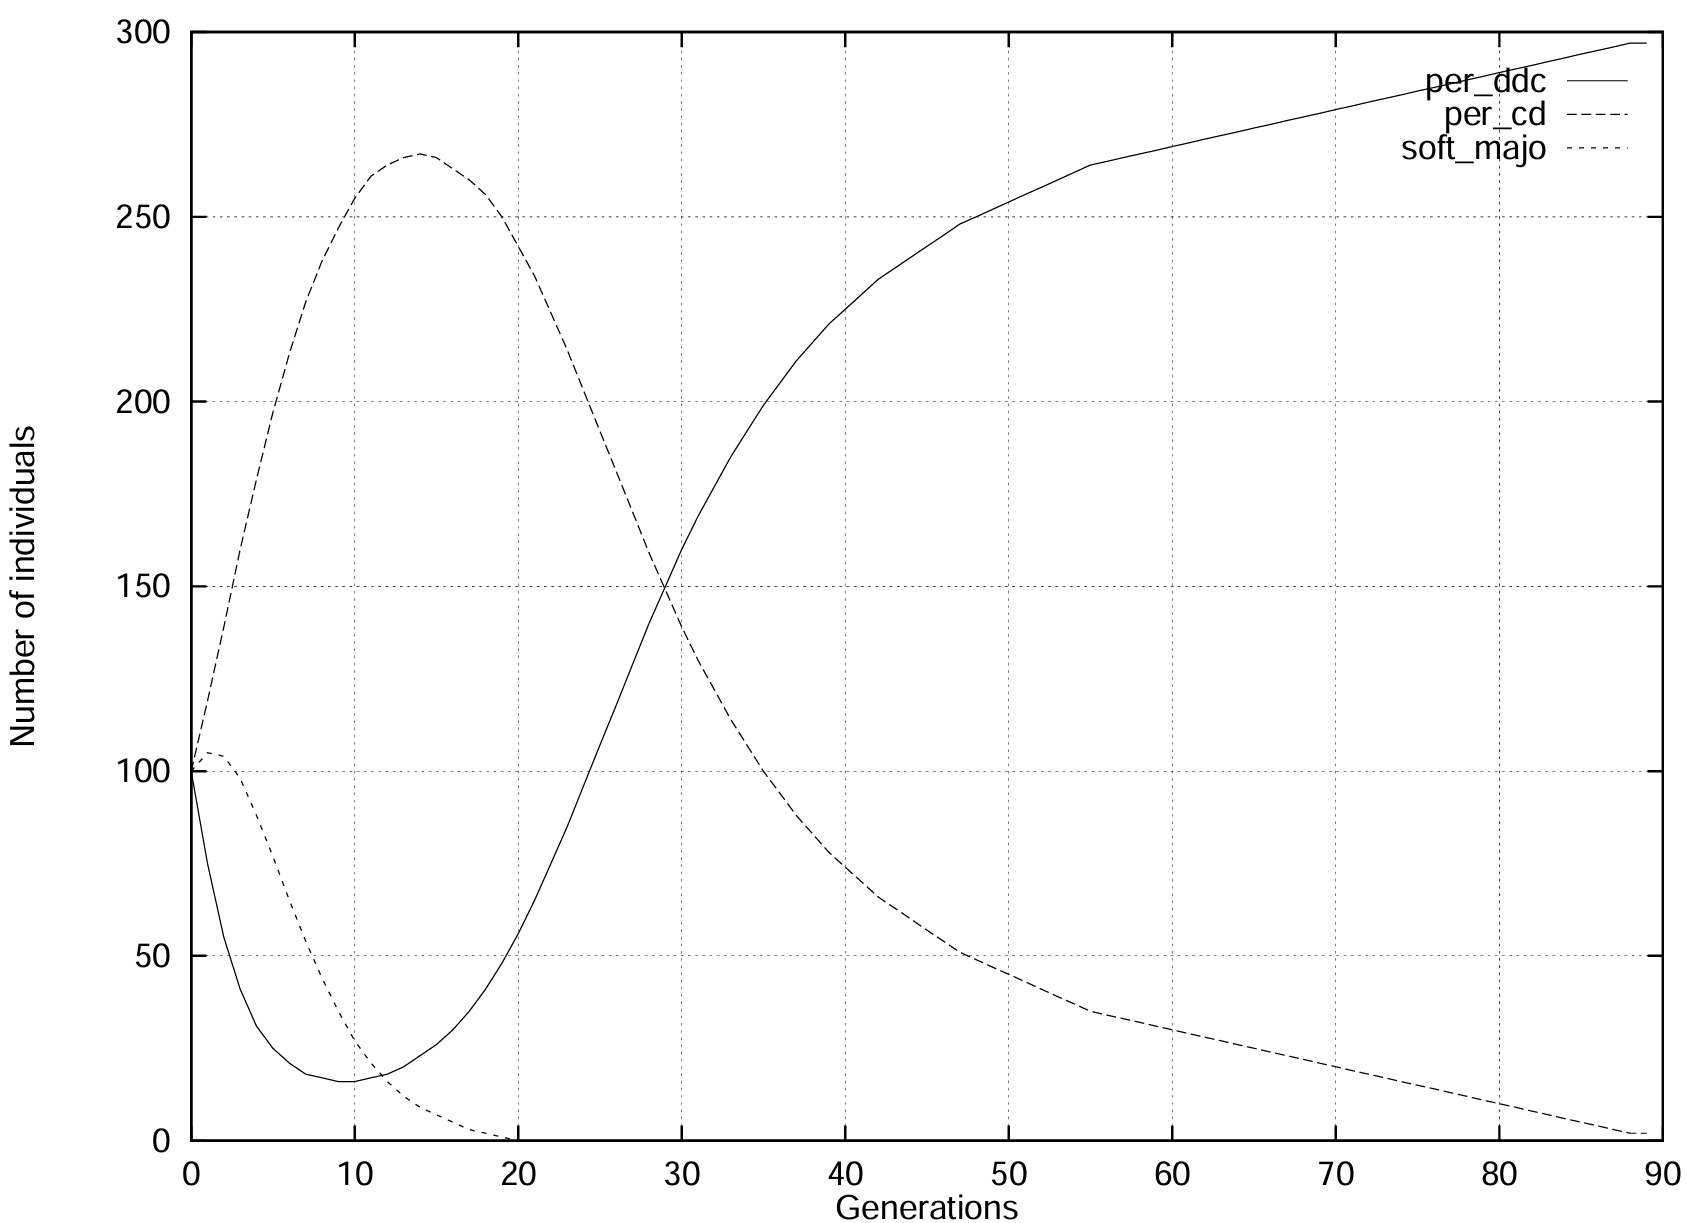
\includegraphics[width=0.7\textwidth]{RefPaperFigures/fig1.jpeg}\par\vspace{0.5em}
		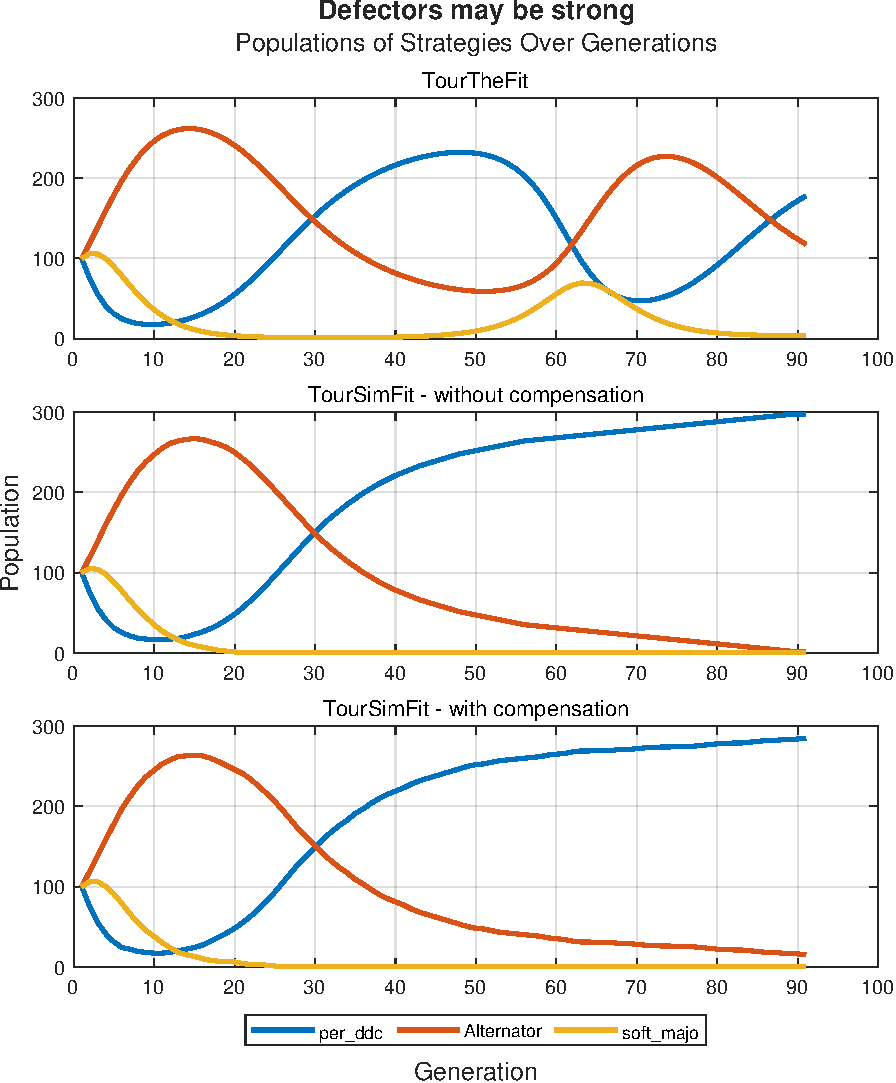
\includegraphics[width=0.7\textwidth]{Defectors may be strong.pdf}
	    \caption{1st Simulation - Defectors may be strong}
	    \label{fig:Defectors may be strong}
	\end{figure}
\subsubsection{2nd Simulation - Monotonous Convergence}
From now on, the results are presented for the simulations used by Mathieu et al. to classify the graphs into 5 categories, the first of which (Figure~\ref{fig:Monotonous Convergence}) is the monotonous convergence of populations. This is the most common form that emerges, as the oscillations presented below are quite sensitive to initial conditions. The results of both the theoretical analysis and the two simulations are identical to those of Mathieu et al., with the only difference being a slightly different final population in the case of \texttt{compensation}, which is again due to the stochastic element. However, the ranking of the strategies remains the same. Run example02 of the Examples folder (after reading Quickstart guide) to recreate the figure.

	\begin{figure}[h]
	    \centering
		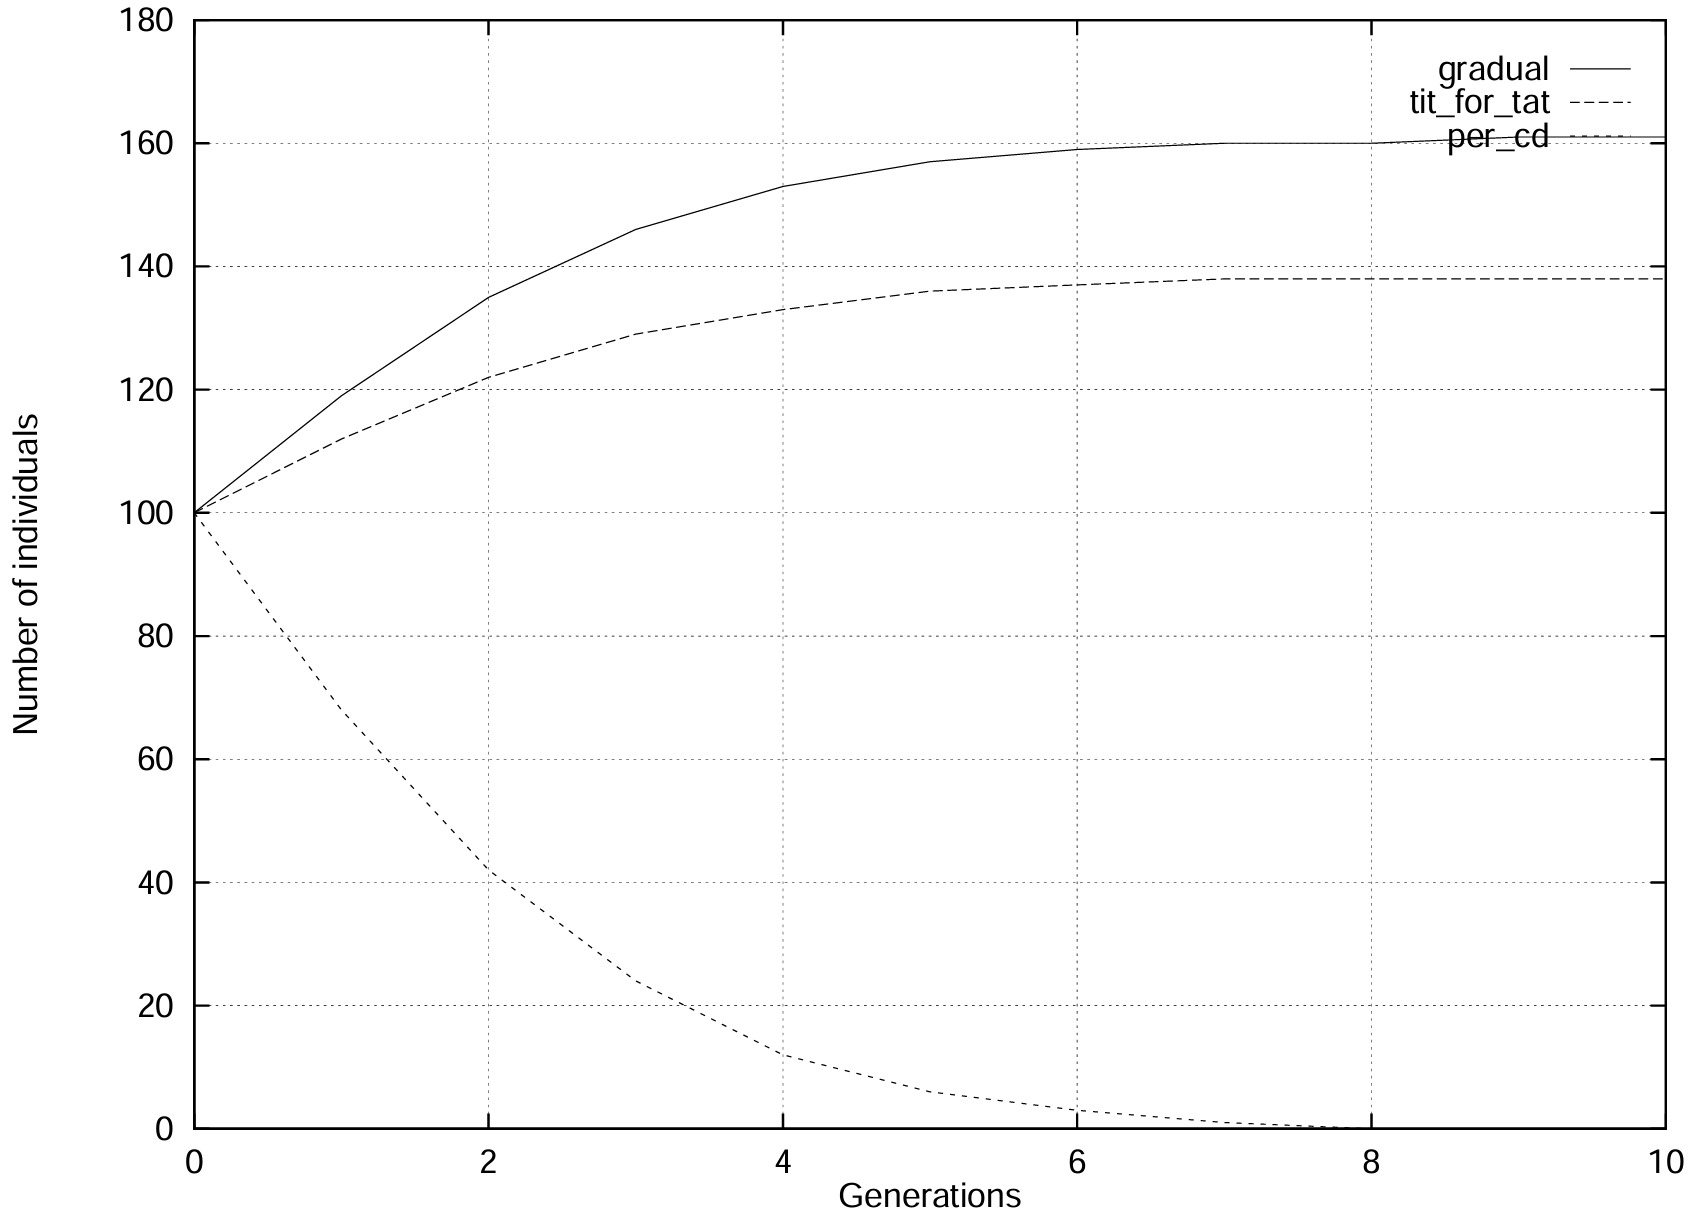
\includegraphics[width=0.7\textwidth]{RefPaperFigures/fig2.jpeg}\par\vspace{0.5em}
	    \includegraphics[width=0.7\textwidth]{Monotonous Convergence.pdf}
	    \caption{2nd Simulation - Monotonous Convergence}
	    \label{fig:Monotonous Convergence}
	\end{figure}
\subsubsection{3rd Simulation - Attenuated Oscillatory movements}
The next category of results from the paper is the diminishing oscillations of populations (Figure~\ref{fig:Attenuated oscillatory movements}). The results in this case are identical to those of Mathieu et al. for all three cases presented. The initial populations in this particular case are quite large, so the one or two players that randomly oppose in the \texttt{compensation} scenario do not significantly affect the trajectory of the function. Run example03 of the Examples folder (after reading Quickstart guide) to recreate the figure.

	\begin{figure}[h]
	    \centering
		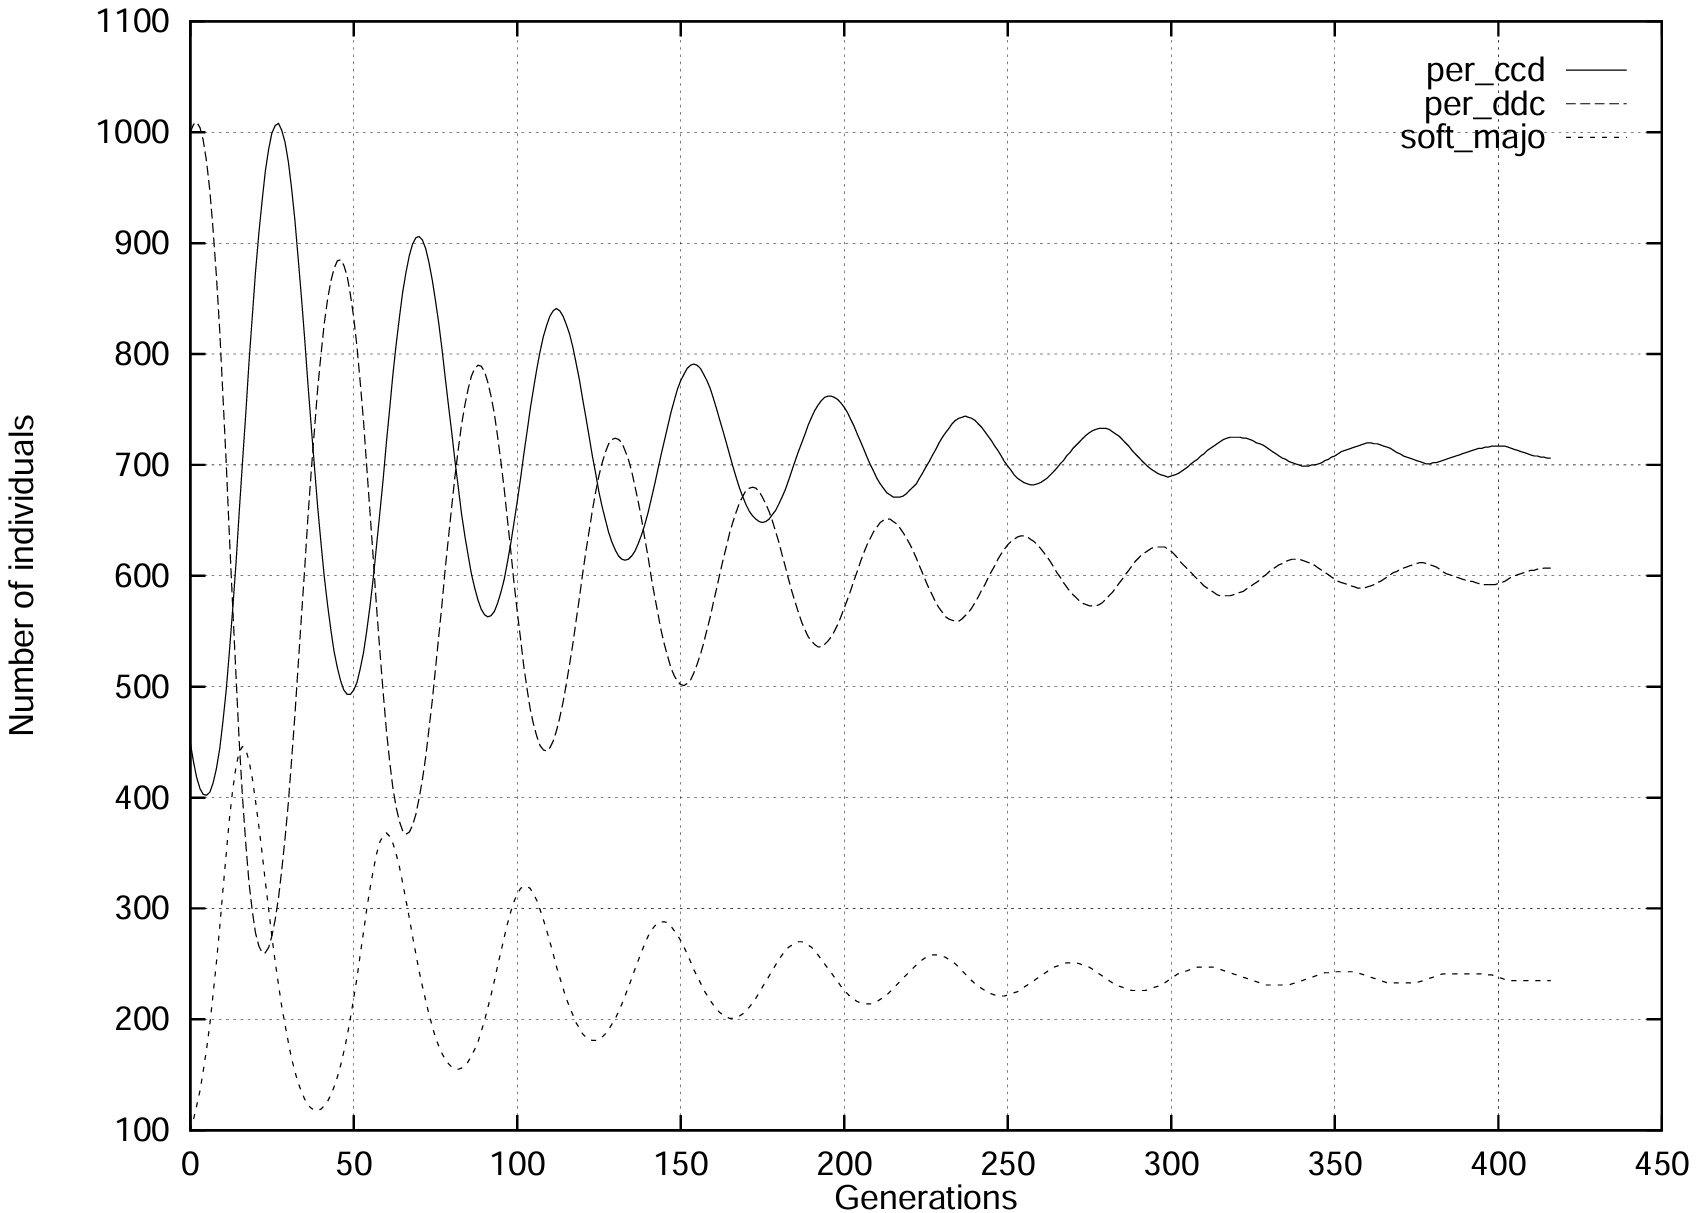
\includegraphics[width=0.7\textwidth]{RefPaperFigures/fig3.jpeg}\par\vspace{0.5em}
	    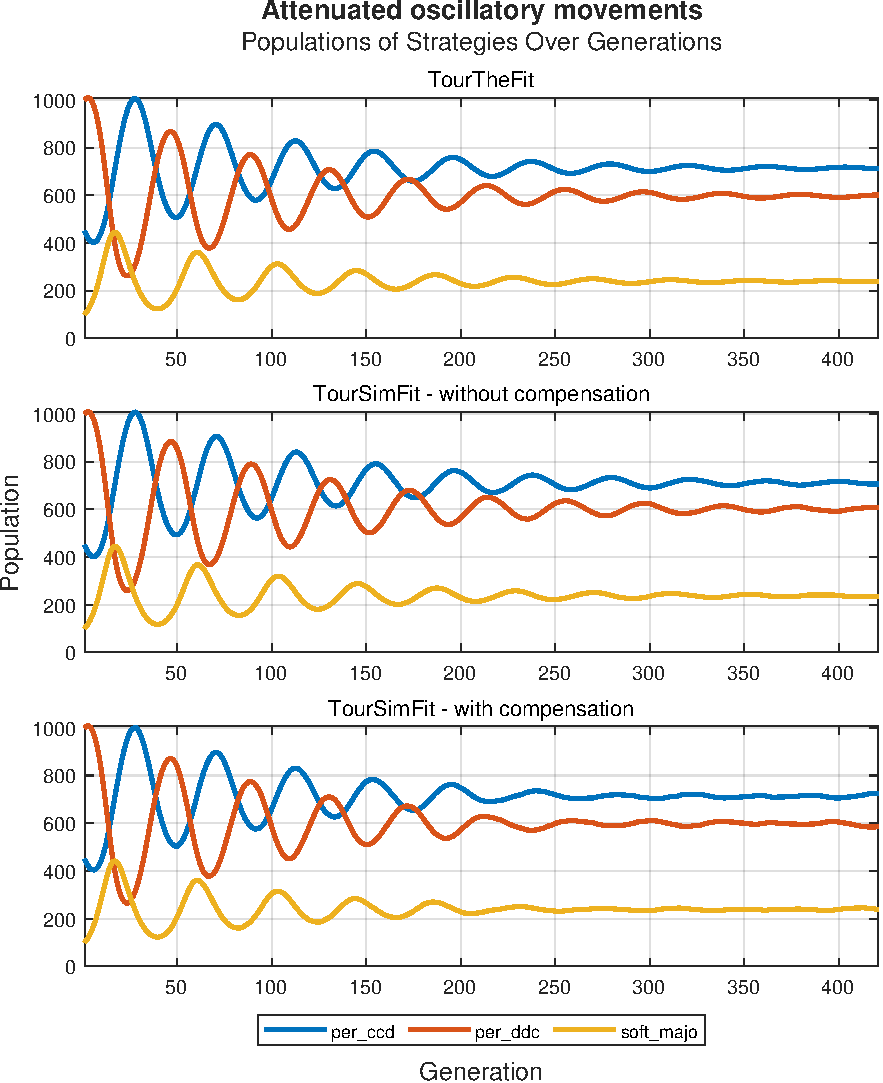
\includegraphics[width=0.7\textwidth]{Attenuated oscillatory movements.pdf}
	    \caption{3rd Simulation - Attenuated oscillatory movements}
	    \label{fig:Attenuated oscillatory movements}
	\end{figure}
\subsubsection{4th Simulation - Periodic movements}
The third case is the appearance of periodic movements/oscillations (Figure~\ref{fig:Periodic movements}), without an increase or decrease in the amplitude of the oscillations. This behavior generally appears when there are three strategies with a "rock-paper-scissors" logic: the 1st "beats" the 2nd, which "beats" the 3rd, which in turn "beats" the 1st. In this particular case, \texttt{per\_ccd} beats \texttt{soft\_majo}, which beats \texttt{per\_ddc}, which beats \texttt{per\_ccd}. With appropriate initial populations, the following results are observed. The theoretical analysis shows that the oscillation actually fades — it is a diminishing oscillation as before. This is due to the fact that in discrete cases, such as these simulations, it becomes certain through suitable choices that the system will return to a previous state, and thus repetition/oscillation will occur. However, in the theoretical analysis, this does not happen (due to the "infinity" of states because of decimal numerics), and thus the oscillation is damped. The \texttt{TourSimFit} function without \texttt{compensation} again yields results identical to those of Mathieu et al., while the case with \texttt{compensation}, although visually less appealing, also captures the oscillation, even with noticeable noise due to randomness (the amplitudes of the oscillations are small, so even the addition of one or two extra players has a noticeable effect). Run example04 of the Examples folder (after reading Quickstart guide) to recreate the figure.

	\begin{figure}[h]
	    \centering
		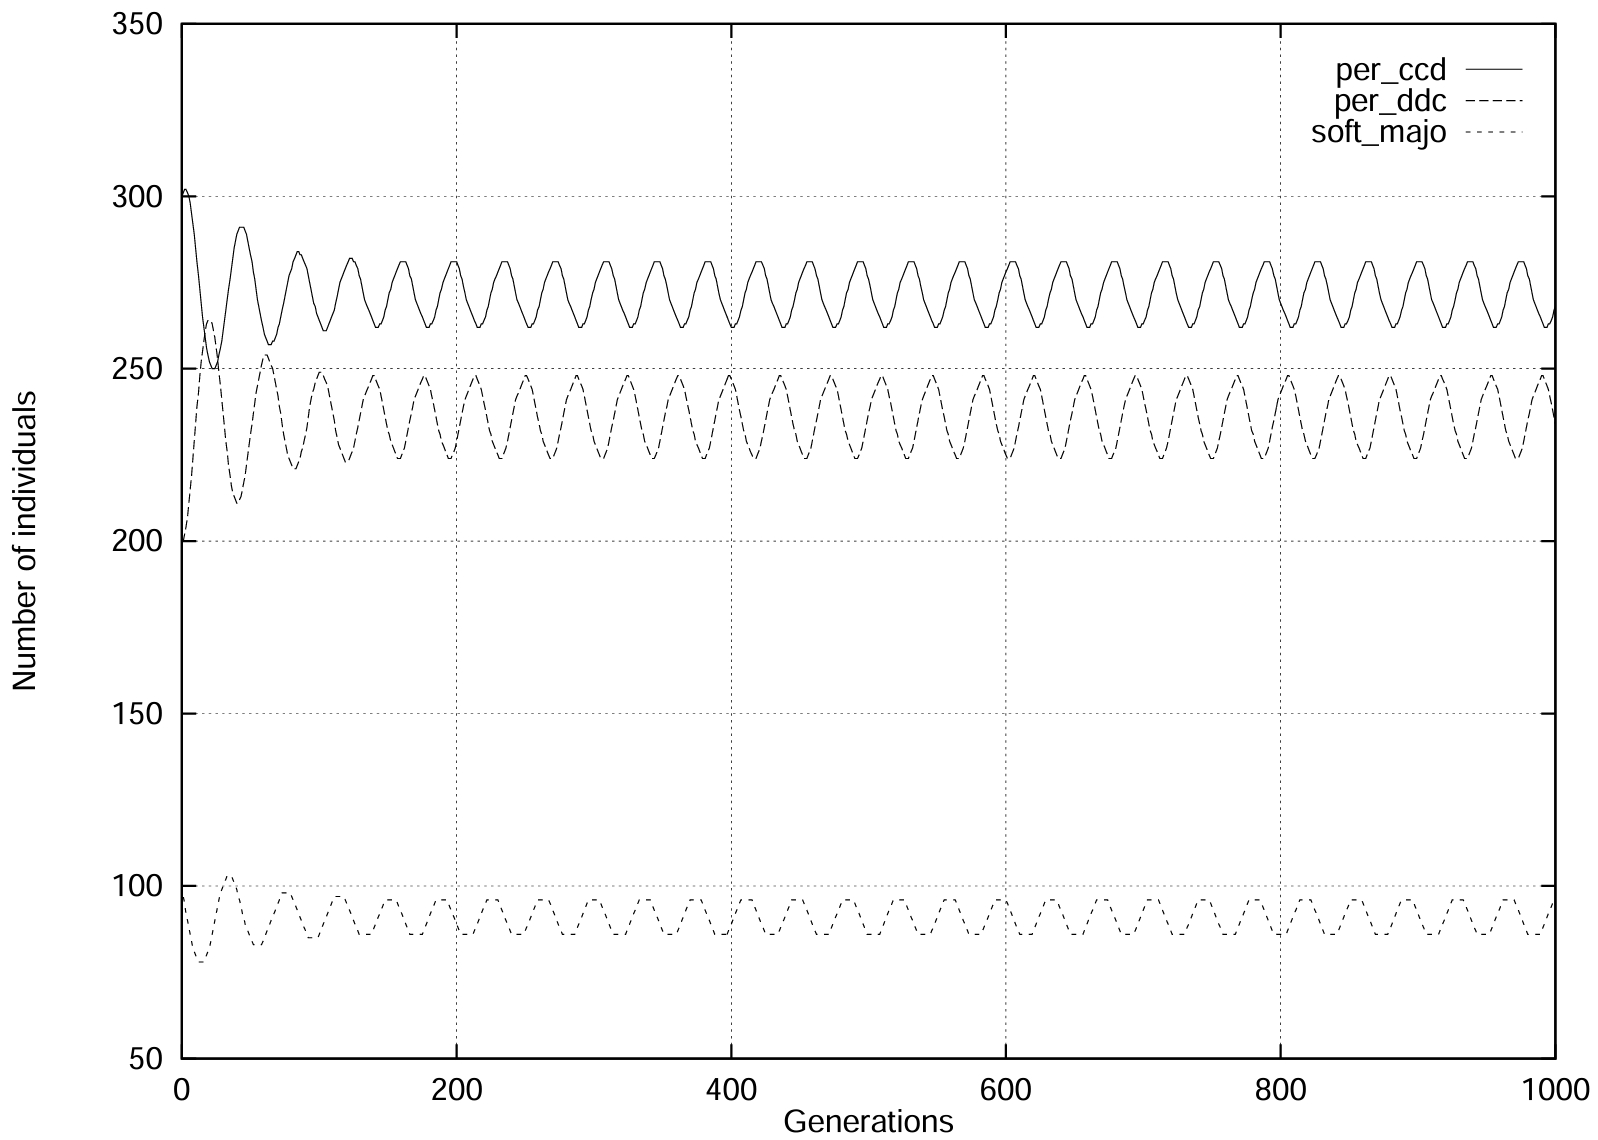
\includegraphics[width=0.7\textwidth]{RefPaperFigures/fig4.jpeg}\par\vspace{0.5em}
	    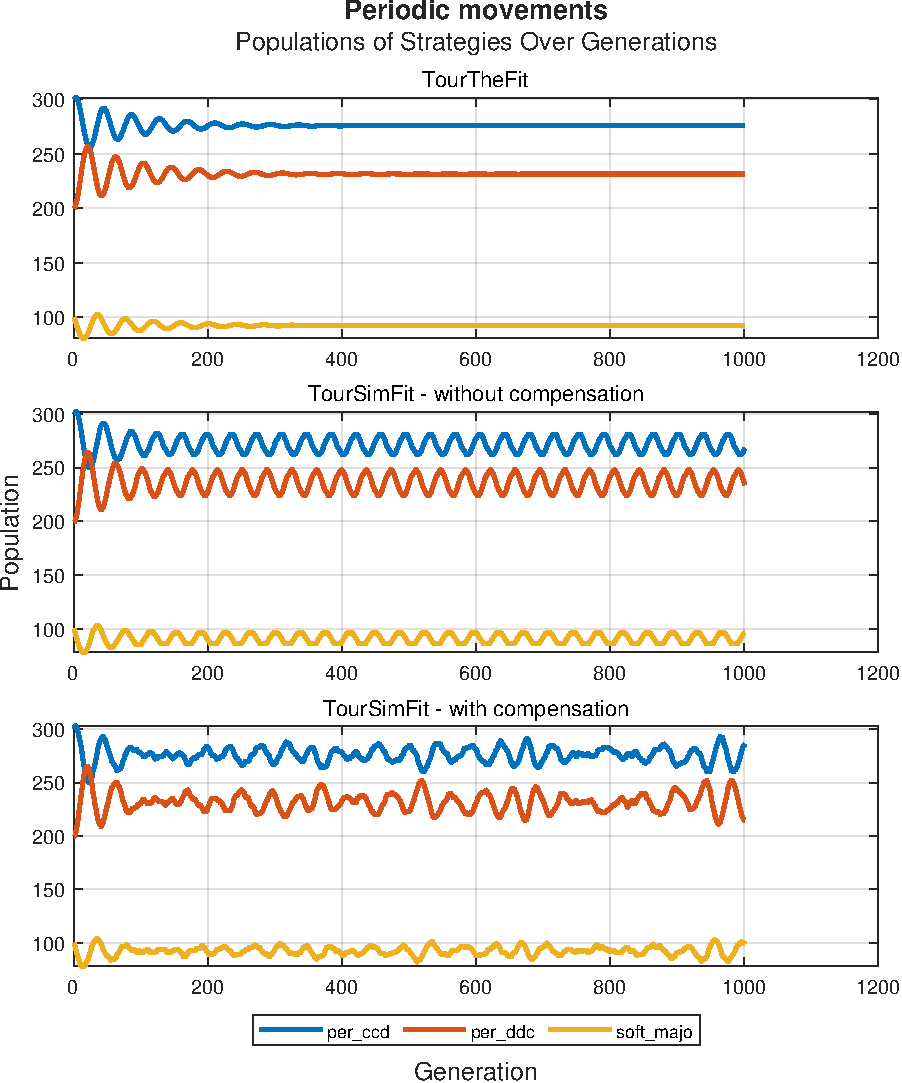
\includegraphics[width=0.7\textwidth]{Periodic movements.pdf}
	    \caption{4th Simulation - Periodic movements}
	    \label{fig:Periodic movements}
	\end{figure}
\subsubsection{5th Simulation - Increasing oscillations}
One of the most unexpected cases is that of increasing oscillations (Figure~\ref{fig:Increasing oscillations}). With an appropriate choice of the payoff matrix, strategies, and initial populations, this phenomenon can be observed.

 A result very similar to that of the paper was observed in the case of \texttt{TourSimFit} without \texttt{compensation}. However, for the cases of \texttt{TourTheFit} and \texttt{TourSimFit} with \texttt{compensation}, diminishing oscillations are observed, revealing two truths about the cases of increasing oscillations. First, they arise from populations capable of exhibiting normal oscillations, with a suitable modification of the payoff matrix. Second, they are particularly sensitive cases that collapse back into normal or diminishing oscillations with even a slight modification of the dynamics (such as the logic of \texttt{compensation}). It is quite possible that for an appropriate choice of \( B \), the cases of \texttt{TourTheFit} and \texttt{TourSimFit} with \texttt{compensation} could also transform into increasing oscillations, but it was considered more important for this work to present this divergence in the results. Run example05 of the Examples folder (after reading Quickstart guide) to recreate the figure.

	\begin{figure}[h]
	    \centering
		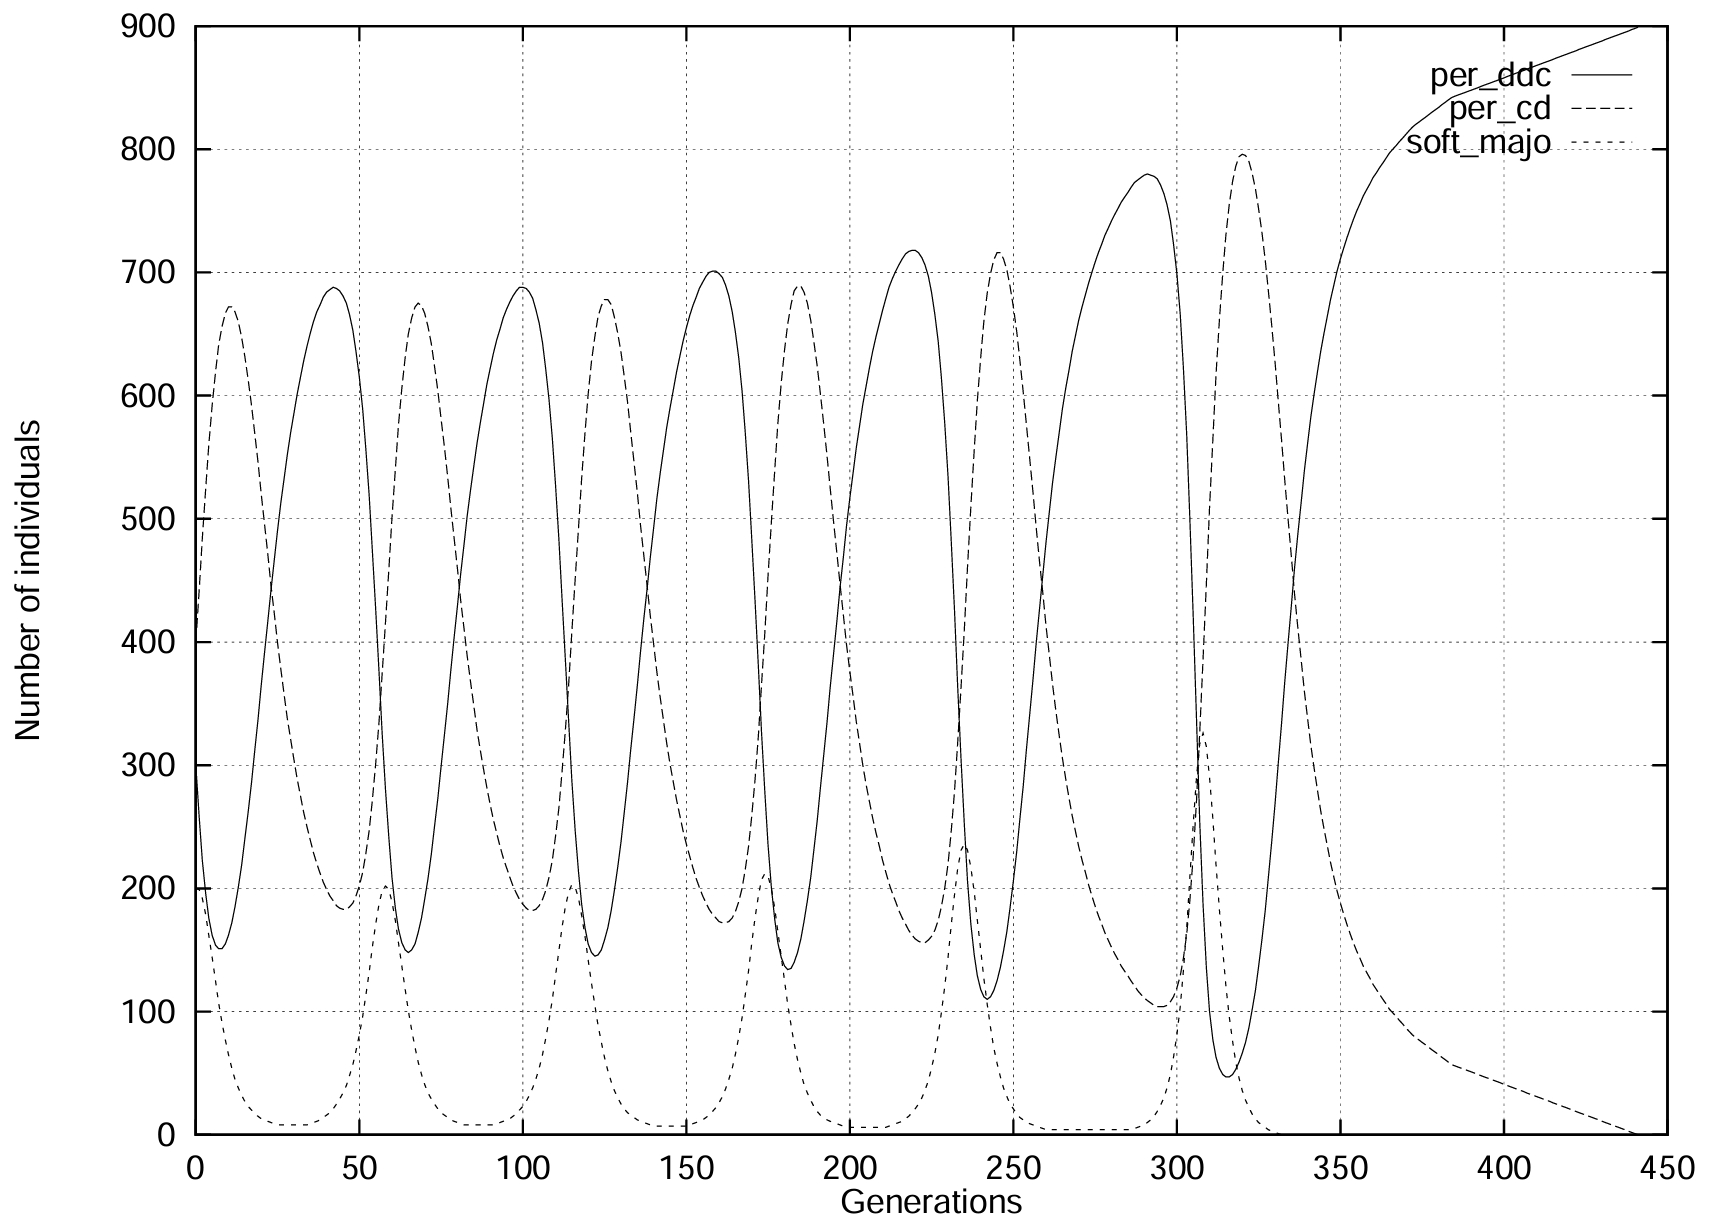
\includegraphics[width=0.7\textwidth]{RefPaperFigures/fig5.jpeg}\par\vspace{0.5em}
	    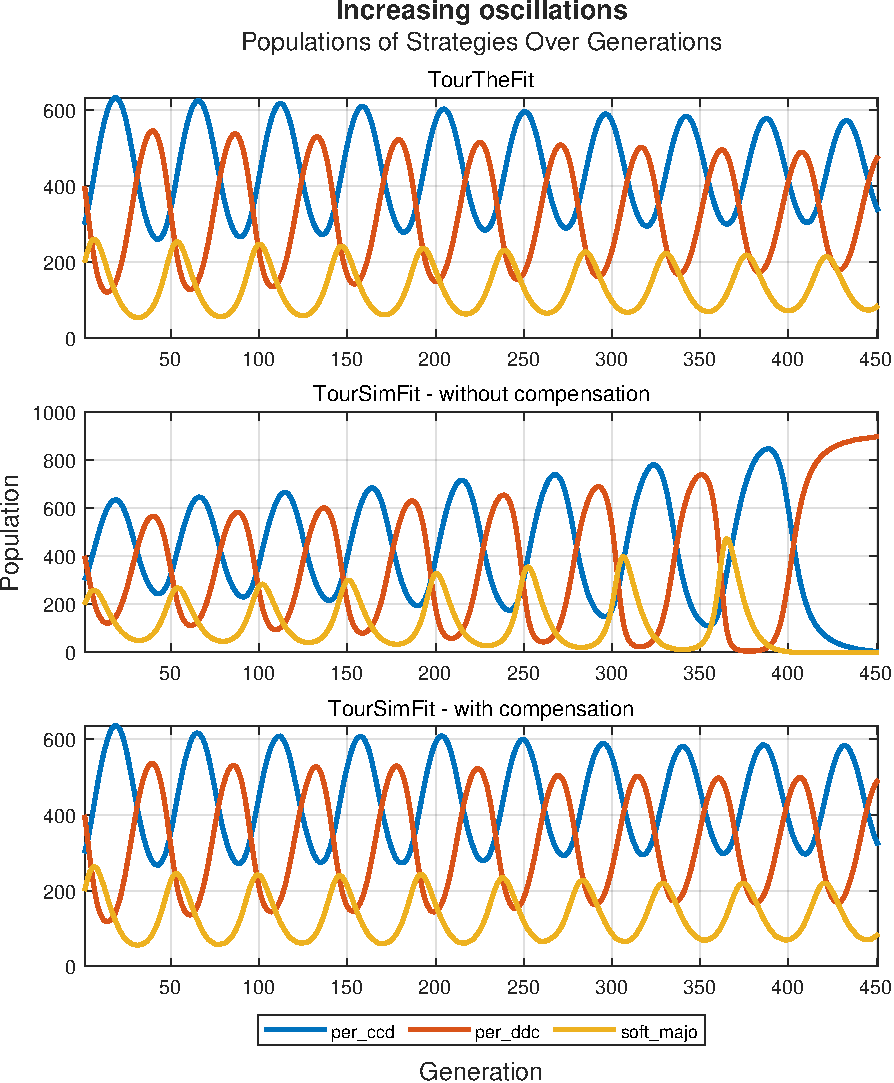
\includegraphics[width=0.7\textwidth]{Increasing oscillations.pdf}
	    \caption{5th Simulation - Increasing oscillations}
	    \label{fig:Increasing oscillations}
	\end{figure}
\subsubsection{6th Simulation - Chaos/Disordered oscillations}
The last case presented in the paper is that of disordered oscillations (Figure~\ref{fig:Disordered oscillations}). The authors of the paper rightly hesitate to characterize it as a truly chaotic case because, due to the discrete nature of the simulation, any such behavior after a sufficient number of generations either reaches equilibrium or simply repeats. However, the results of this particular simulation appear quite chaotic. Again, the case of \texttt{TourSimFit} without \texttt{compensation} fully matches the results of the paper. In contrast, due to the sensitivity of the phenomenon, the cases of the theoretical analysis and the actual simulation with \texttt{compensation} differ significantly, as they do not exhibit the chaotic behavior around generation 140 as in the case of the paper. Nevertheless, they predict the survival of the \texttt{per\_ccccd} and \texttt{Prober} strategies, as well as the values toward which the populations in the \texttt{TourSimFit} case without simulation seem to tend. Run example06 of the Examples folder (after reading Quickstart guide) to recreate the figure.

	\begin{figure}[h]
	    \centering
		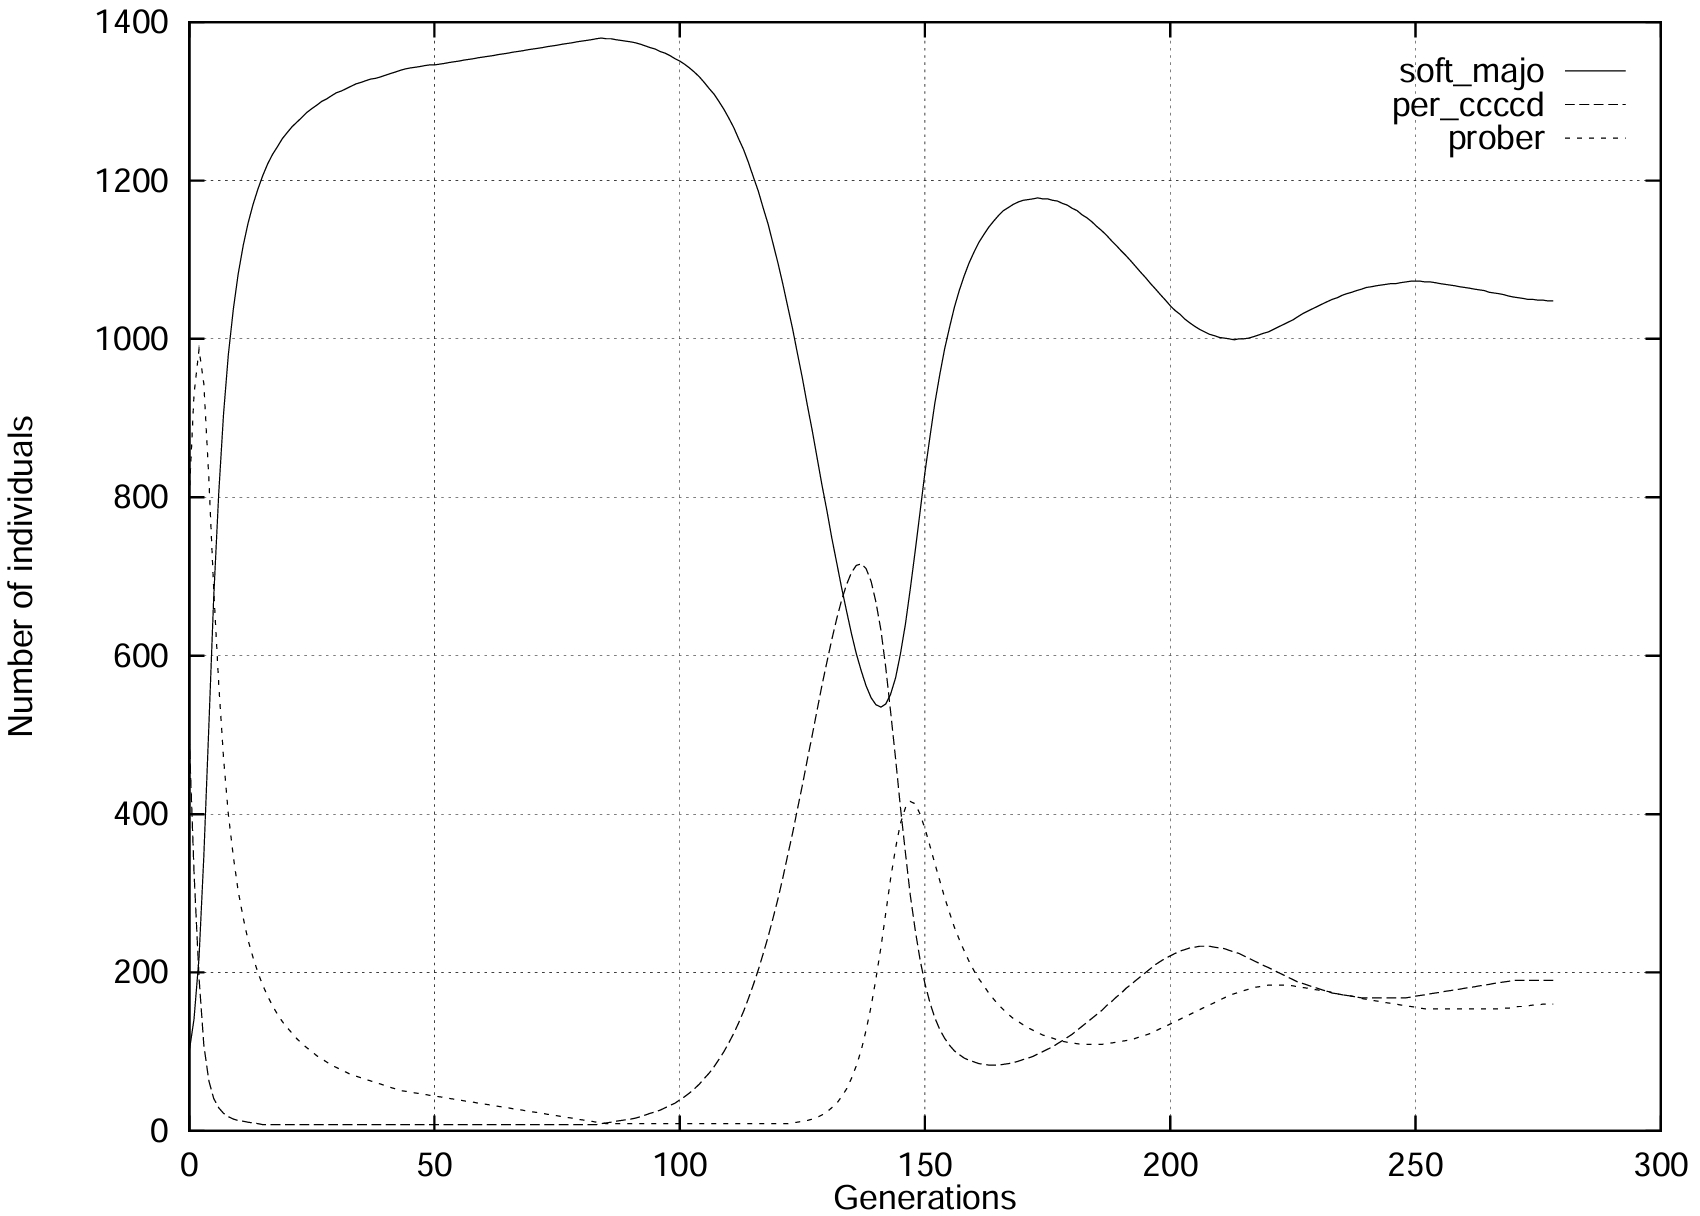
\includegraphics[width=0.7\textwidth]{RefPaperFigures/fig6.jpeg}\par\vspace{0.5em}
	    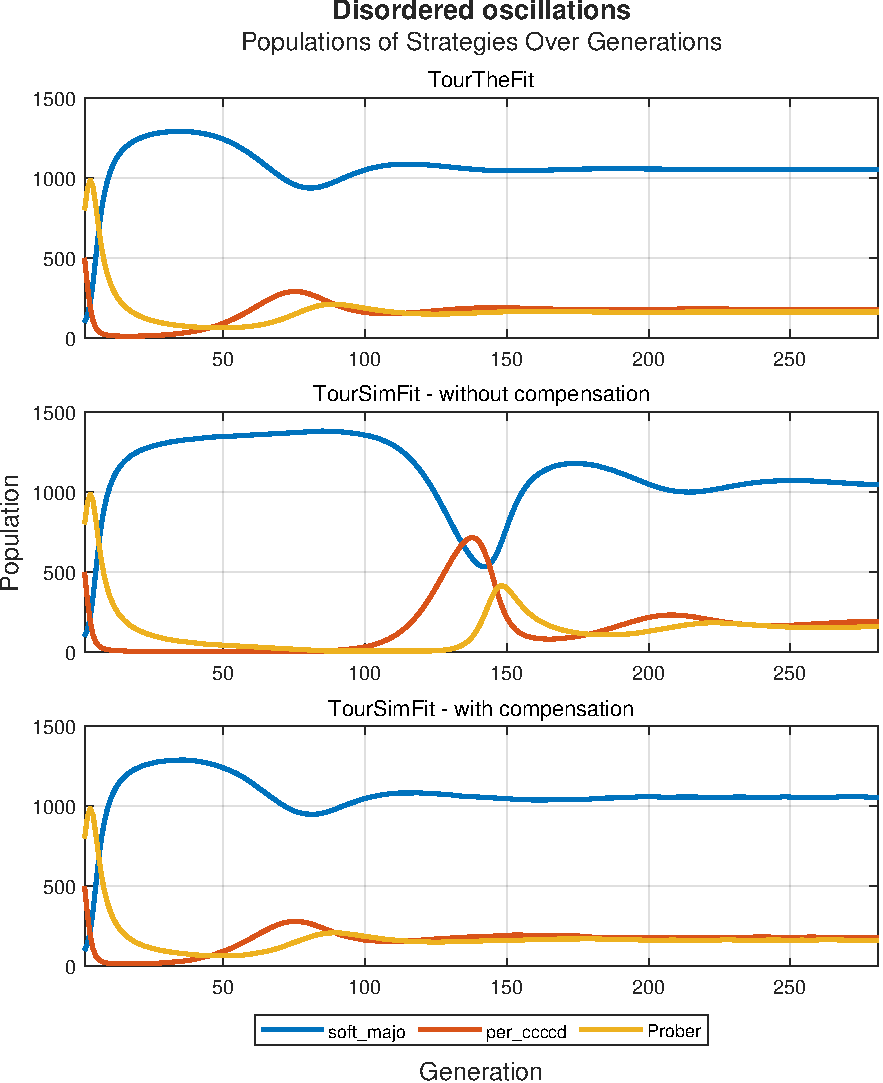
\includegraphics[width=0.7\textwidth]{Disordered oscillations.pdf}
	    \caption{6th Simulation - Disordered oscillations}
	    \label{fig:Disordered oscillations}
	\end{figure}

\subsubsection{7th Simulation - Sensitivity of dynamics to population's size - First Simulation}
From now on, the simulations showcase the sensitivity of the results to the initial conditions of the examples. Again, the results presented are compared to the results of Mathieu et al and any differences are discussed. The first simulation aims to present the sensitivity of the dynamics to the initial population's size for each strategy. More specifically, the same set of strategies can lead to many different forms of dynamics occuring, depending on the population of each of the strategy. This should not come as a surprise, as even in the previous examples the strategies used were often the same, with the differences in dynamics being caused by different initial populations. In this first example (Figure~\ref{fig:Sensitivity of dynamics to population's size - First Simulation}), the result is a periodic movement, which is also recreated in the TourSimFit without compensation, as well as (mostly) in the TourSimFit with compensation. However, the theoretical result of TourTheFit is an attenuated oscillation, as in the case of the Figure~\ref{fig:Periodic movements}, for the same reasons as before. Run example07 of the Examples folder (after reading Quickstart guide) to recreate the figure.

	\begin{figure}[h]
	    \centering
		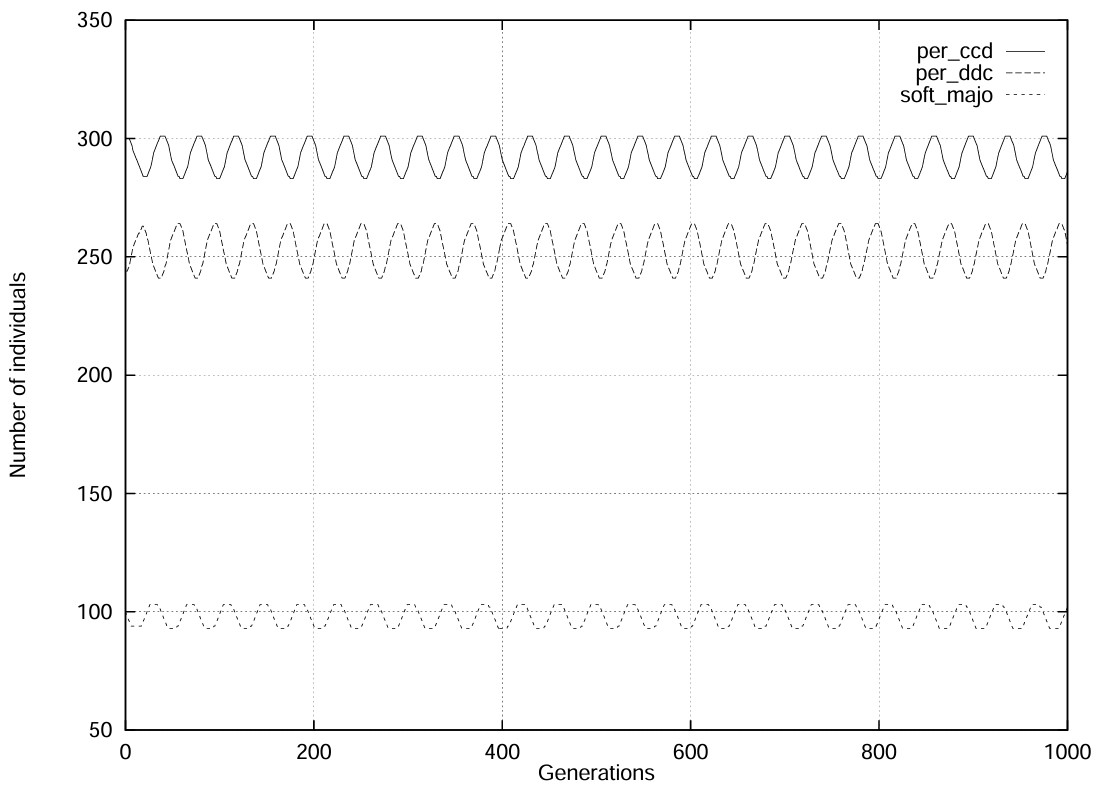
\includegraphics[width=0.7\textwidth]{RefPaperFigures/fig7a.jpeg}\par\vspace{0.5em}
	    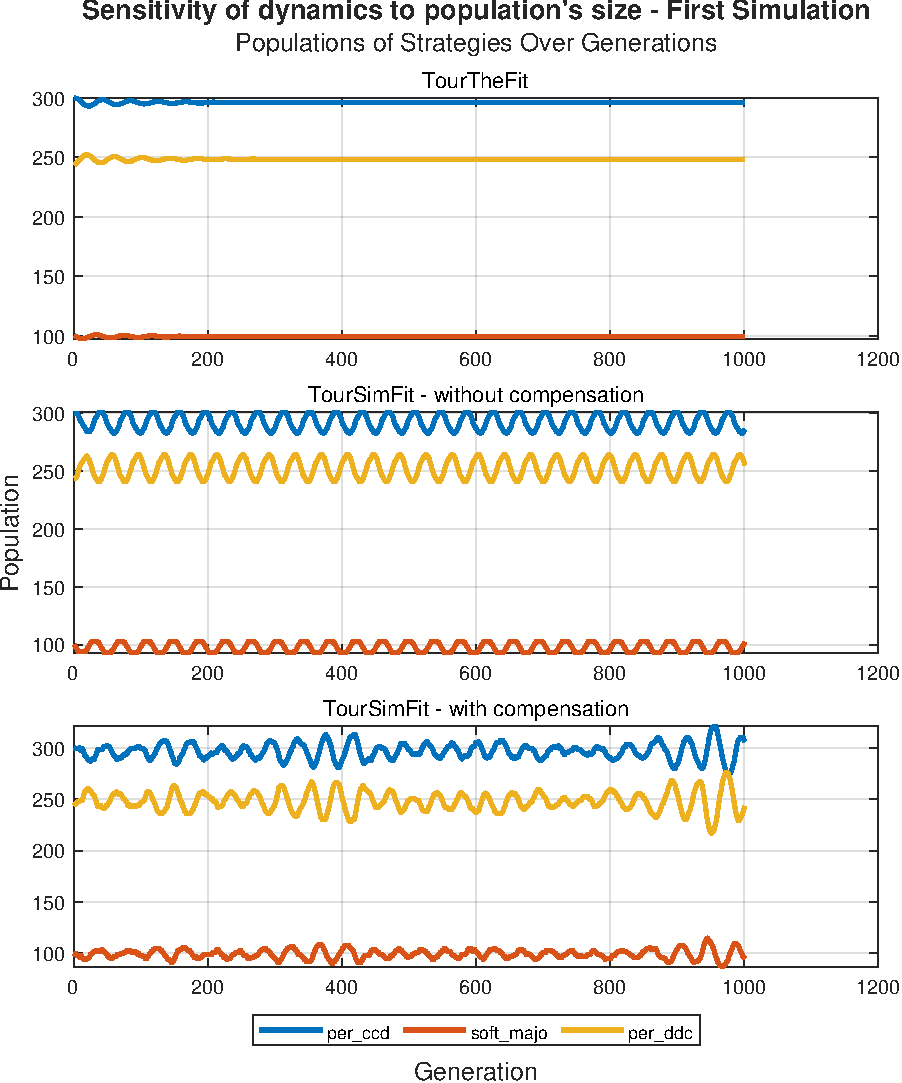
\includegraphics[width=0.7\textwidth]{Sensitivity of dynamics to population's size - First Simulation.pdf}
	    \caption{7th Simulation - Sensitivity of dynamics to population's size - First Simulation}
	    \label{fig:Sensitivity of dynamics to population's size - First Simulation}
	\end{figure}
\subsubsection{8th Simulation - Sensitivity of dynamics to population's size - Second Simulation}
The second example of the showcase of the sensitivity of the dynamics to the population's size shows a monotonous convergence that is caused by a slight differentiation in the initial population vector of the previous simulation. The only difference between this simulation and the previous one is one extra \texttt{per\_ddc} added, which ends up being enough to change the resulting dynamics completely. This is recreated (Figure~\ref{fig:Sensitivity of dynamics to population's size - Second Simulation}) in the case of TourSimFit without compensation. However, in the cases of TourTheFit there appears to still be a slight attenuated oscillation, meaning the convergence is not monotonous, and in the case of the TourSimFit with compensation the result is still a periodic movement, obviously caused by the random element of this method. Thus, we observe a large sensitivity of the dynamics to the repartition method of the population, which is also discussed in a later example. Run example08 of the Examples folder (after reading Quickstart guide) to recreate the figure.

	\begin{figure}[h]
	    \centering
		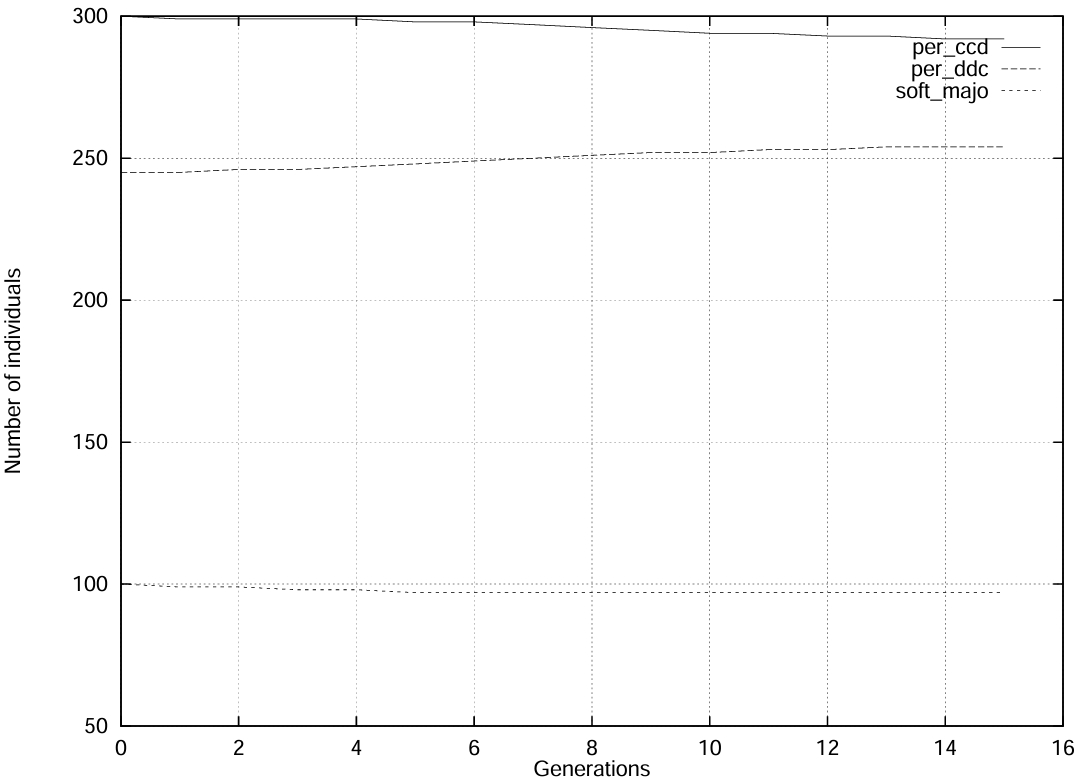
\includegraphics[width=0.7\textwidth]{RefPaperFigures/fig7b.jpeg}\par\vspace{0.5em}
	    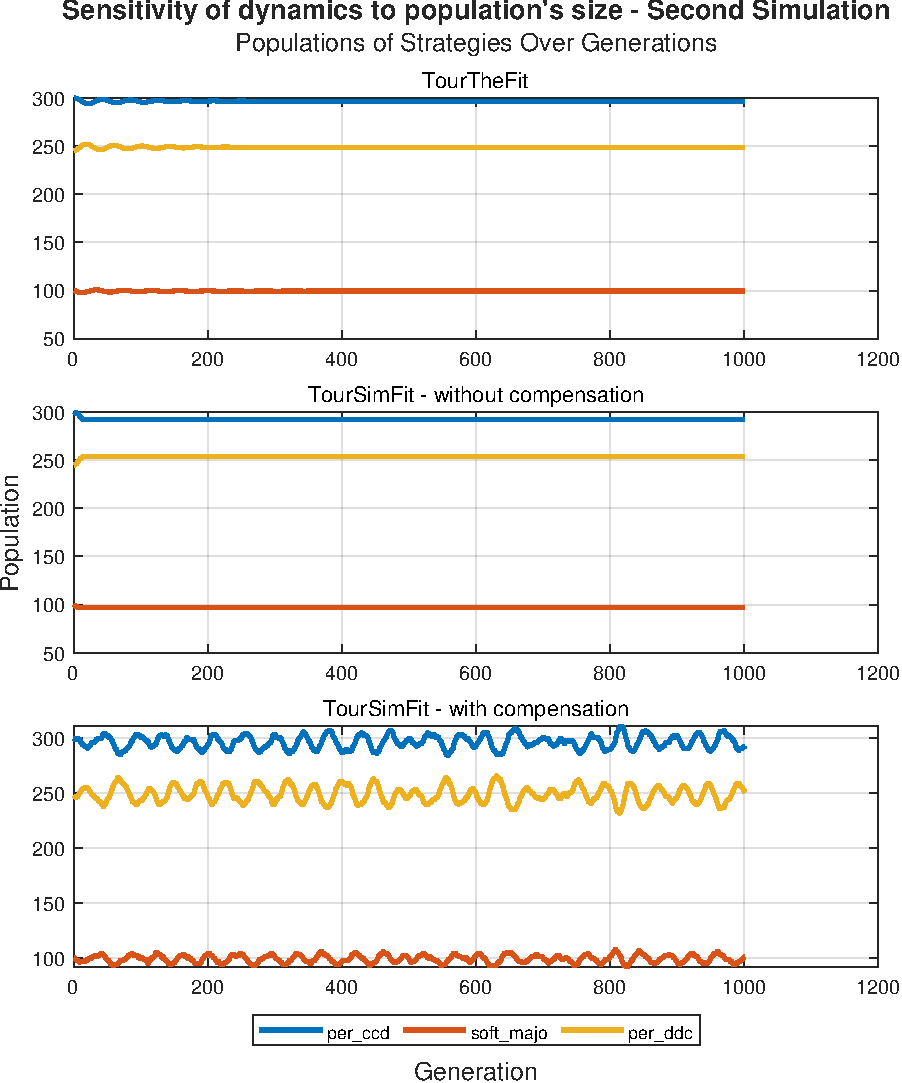
\includegraphics[width=0.7\textwidth]{Sensitivity of dynamics to population's size - Second Simulation.pdf}
	    \caption{8th Simulation - Sensitivity of dynamics to population's size - Second Simulation}
	    \label{fig:Sensitivity of dynamics to population's size - Second Simulation}
	\end{figure}
\subsubsection{9th Simulation - Sensitivity of winner to population's size - First Simulation}
The second case presented is the sensitivity of the winner to the population's size, with winner being the strategy that ends up having the most members of the population at the end of the simulation. This may not be obvious at first; we have seen a lot of cases where the change in dynamics is clearly visible but the ensuing winner still remains the same in most cases. The first example (Figure~\ref{fig:Sensitivity of winner to population's size - First Simulation}) shows an initial population that ultimately announces \texttt{per\_ddc} as the winning strategy; the winner is recreated by each of our own methods, however the dynamics in the case of TourTheFit are visibly different, due to the population of \texttt{soft\_majo} never actually dying out and thus making the \texttt{Alternator} strategy more viable (as we covered, \texttt{Alternator} is the perfect counter to \texttt{soft\_majo}). Run example09 of the Examples folder (after reading Quickstart guide) to recreate the figure.
	\begin{figure}[h]
	    \centering
		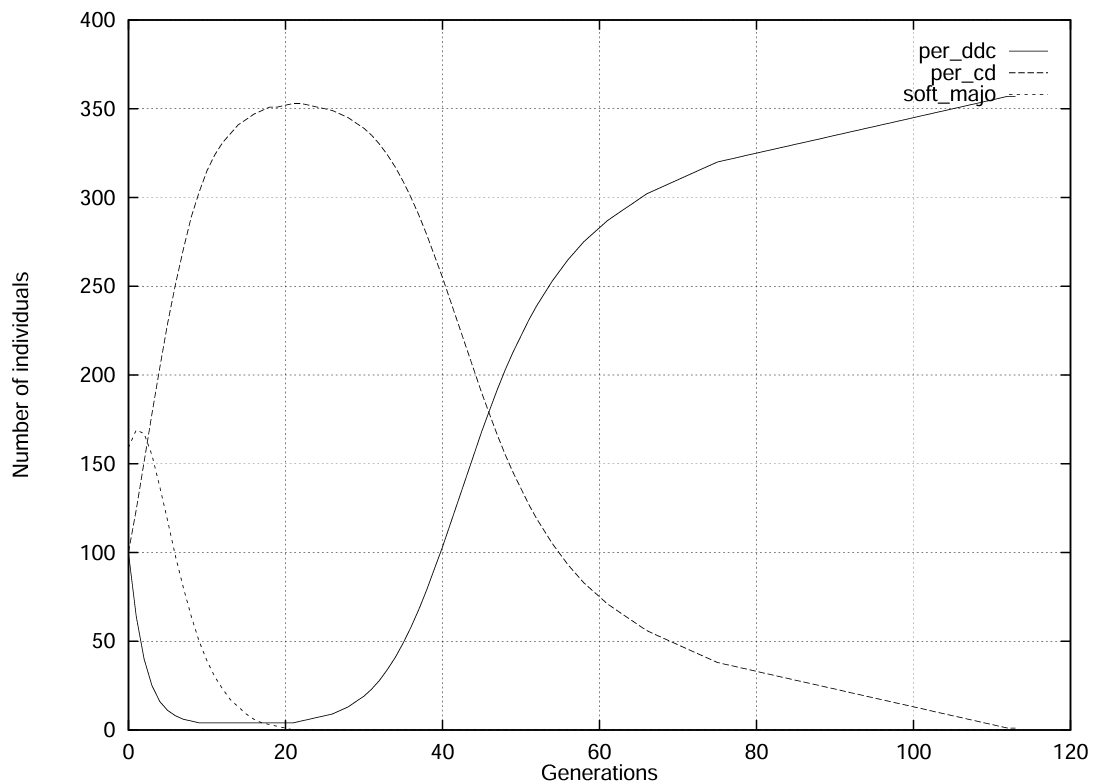
\includegraphics[width=0.7\textwidth]{RefPaperFigures/fig8a.jpeg}\par\vspace{0.5em}
	    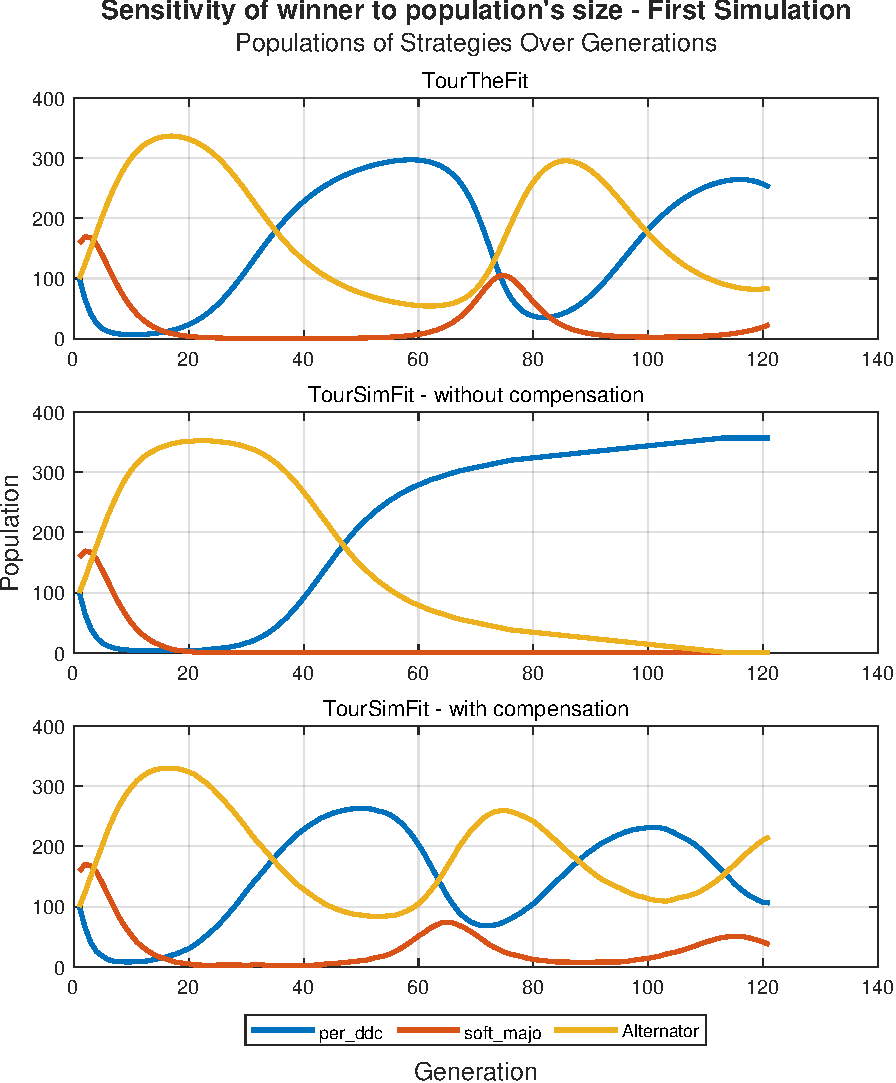
\includegraphics[width=0.7\textwidth]{Sensitivity of winner to population's size - First Simulation.pdf}
	    \caption{9th Simulation - Sensitivity of winner to population's size - First Simulation}
	    \label{fig:Sensitivity of winner to population's size - First Simulation}
	\end{figure}
\subsubsection{10th Simulation - Sensitivity of winner to population's size - Second Simulation}
The second part of the sensitivity of winner to population's size showcase adds one \texttt{soft\_majo} participant to the initial population, making \texttt{Alternator} the winner. The results (Figure~\ref{fig:Sensitivity of winner to population's size - Second Simulation}) are recreated in the case of TourSimFit without compensation. However, in the cases of TourTheFit and TourSimFit with compensation, \texttt{Alternator} does not seem to be the decisive winner of the simulation, since at the end of the simulation there is still a rising population of \texttt{per\_ddc}, strategy which does better versus \texttt{Alternator}, meaning that the eventual winner would be \texttt{per\_ddc}. This in turn is caused by the fact that the population of \texttt{per\_ddc} is not eliminated in these two cases, thus making a comeback possible. Note that, as Mathieu et al suggest, the modified strategy never wins (unless if it was already the winner). Run example10 of the Examples folder (after reading Quickstart guide) to recreate the figure.
	\begin{figure}[h]
	    \centering
		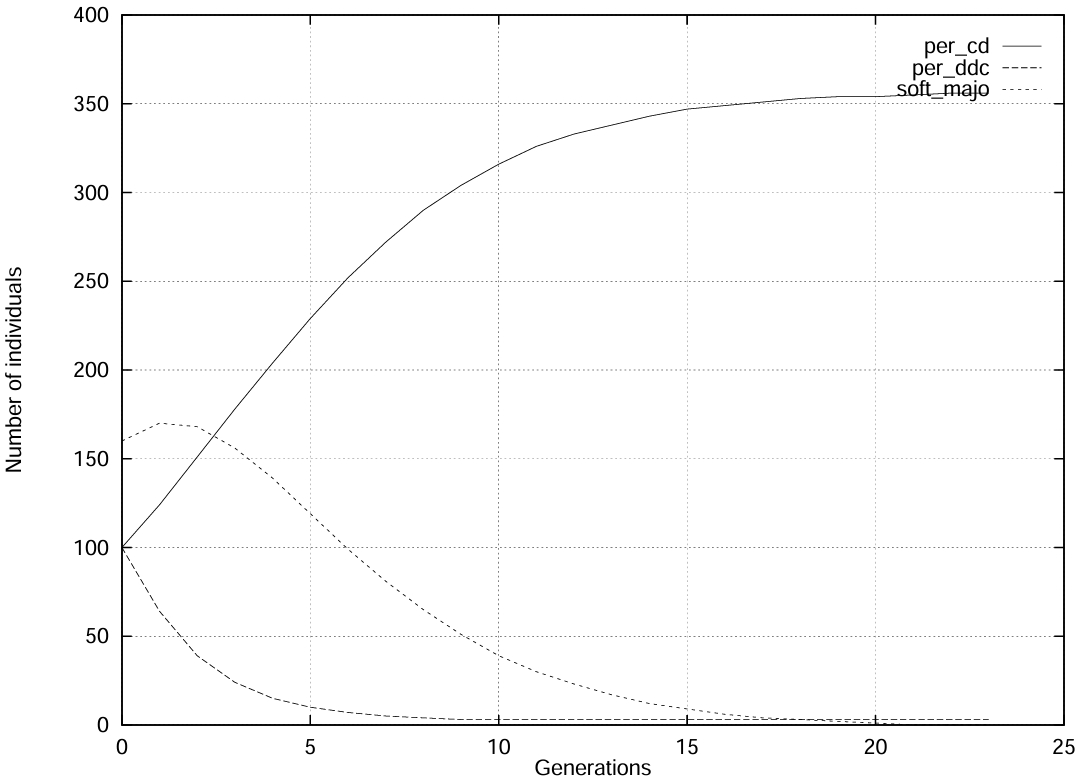
\includegraphics[width=0.7\textwidth]{RefPaperFigures/fig8b.jpeg}\par\vspace{0.5em}
	    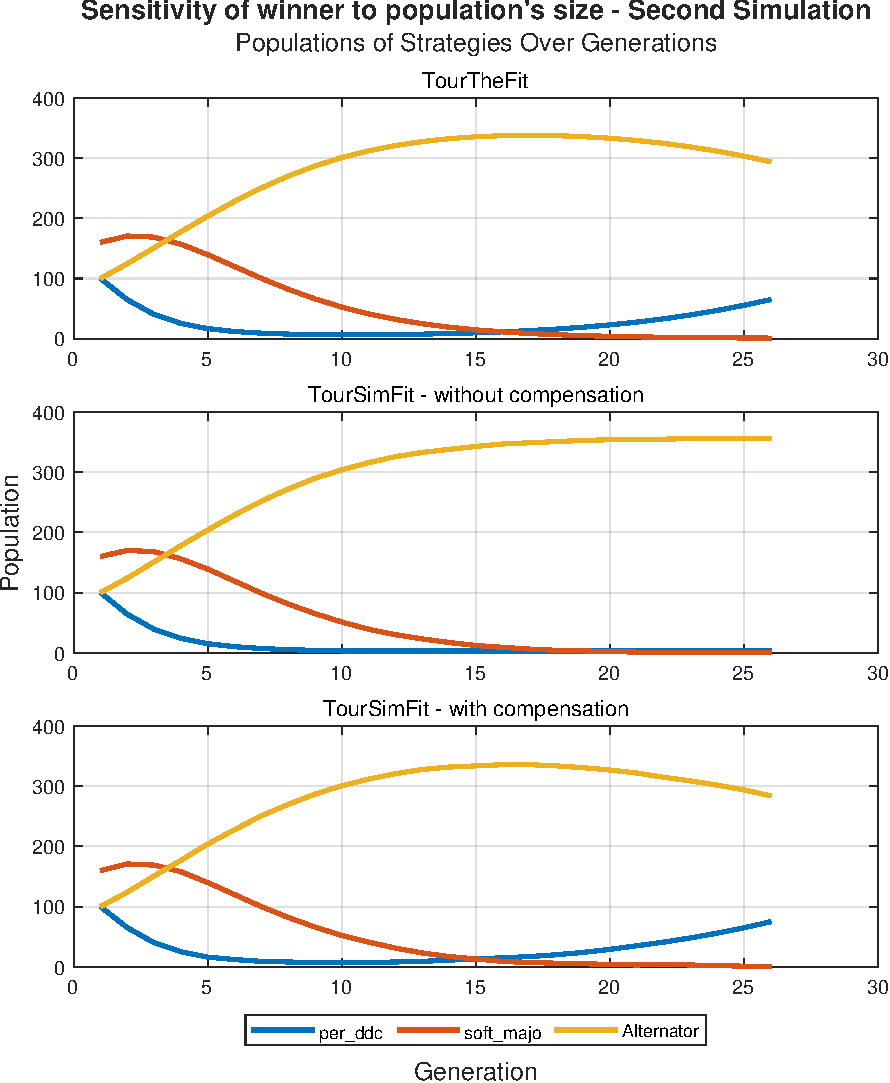
\includegraphics[width=0.7\textwidth]{Sensitivity of winner to population's size - Second Simulation.pdf}
	    \caption{10th Simulation - Sensitivity of winner to population's size - Second Simulation}
	    \label{fig:Sensitivity of winner to population's size - Second Simulation}
	\end{figure}
\subsubsection{11th Simulation - Sensitivity to game length - First Simulation}
The next aspect of initial conditions studied is the game length, meaning the number of rounds each match between two players lasts. As it turns out, periodic strategies like most studied in this project are sensitive to the game length, because of the varying ``winner'' of each match based on the amount of rounds played. In the first part, each match lasts 7 rounds and the result is a periodic movement. This is also recreated (Figure~\ref{fig:Sensitivity to game length - First Simulation}) in the case of TourSimFit without compensation, but it again becomes an attenuated oscillatory movement for the cases of TourTheFit and TourSimFit with compensation, for the same reasons as discussed multiple times (a true periodic movement without making rounding errors in some generations is very sensitive). Run example11 of the Examples folder (after reading Quickstart guide) to recreate the figure.
	\begin{figure}[h]
	    \centering
		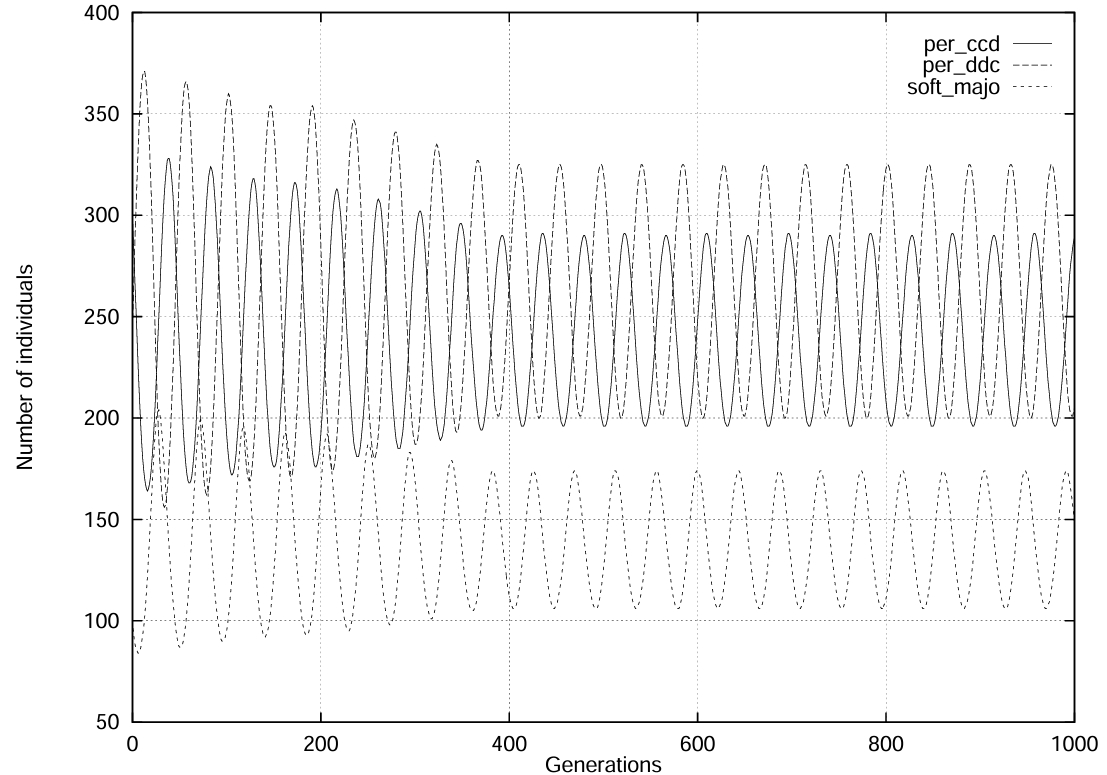
\includegraphics[width=0.7\textwidth]{RefPaperFigures/fig9a.jpeg}\par\vspace{0.5em}
	    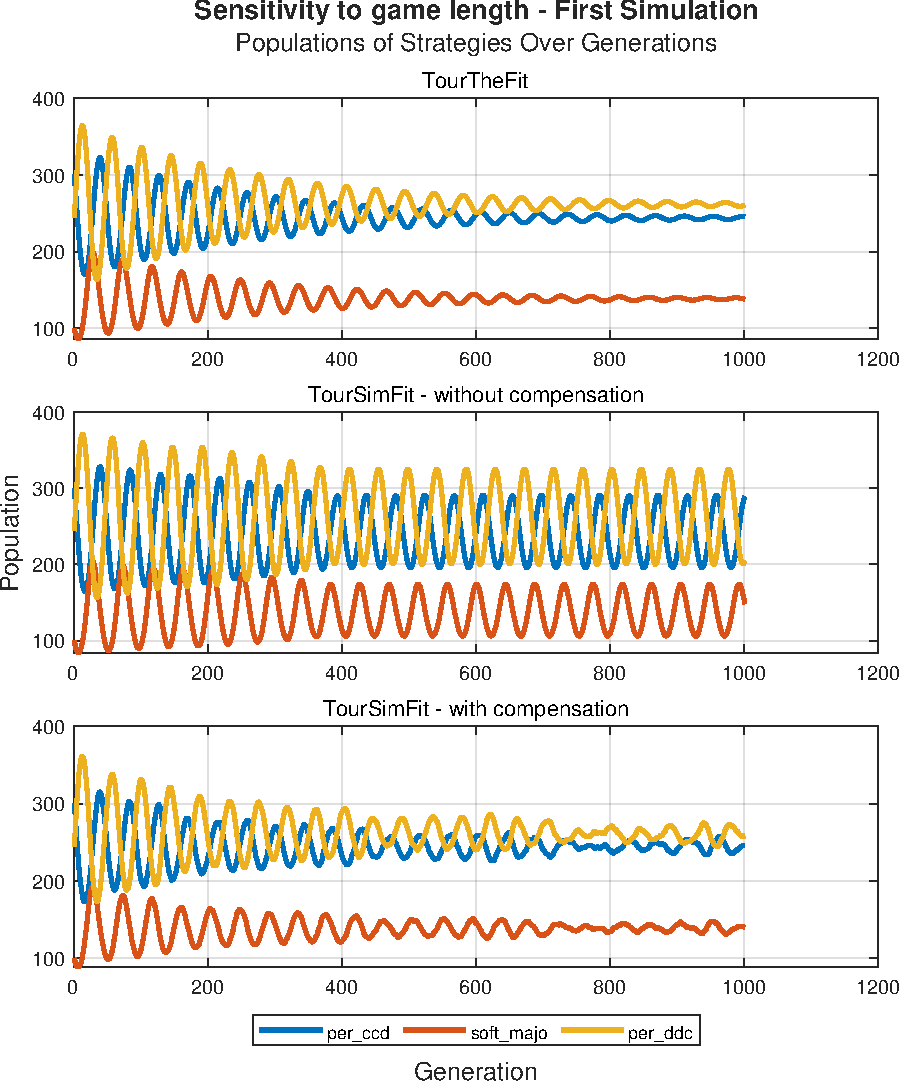
\includegraphics[width=0.7\textwidth]{Sensitivity to game length - First Simulation.pdf}
	    \caption{11th Simulation - Sensitivity to game length - First Simulation}
	    \label{fig:Sensitivity to game length - First Simulation}
	\end{figure}
\subsubsection{12th Simulation - Sensitivity to game length - Second Simulation}
The second simulation of this part changes only the number of rounds played each match to 6. This results in an attenuated oscillatory movement, which is recreated (Figure~\ref{fig:Sensitivity to game length - Second Simulation}) by every function of our own. Thus, it is shown that the dynamics, as well as the eventual winner (since a periodic movement like the one showcased in the previous example has no official winner) are sensitive to the game length, especially when periodic strategies are used. This happens because, for example, in a 6 round game \texttt{per\_ccd} does not lose as hard to \texttt{per\_ddc} as in the case of a 7 round game (it suffers one less ``effective'' defection, meaning an opponent defection met with cooperation). These slight modifications to the score of each match change the fitness score of each strategy enough to create visible changes to the outcome. Run example12 of the Examples folder (after reading Quickstart guide) to recreate the figure.
	\begin{figure}[h]
	    \centering
		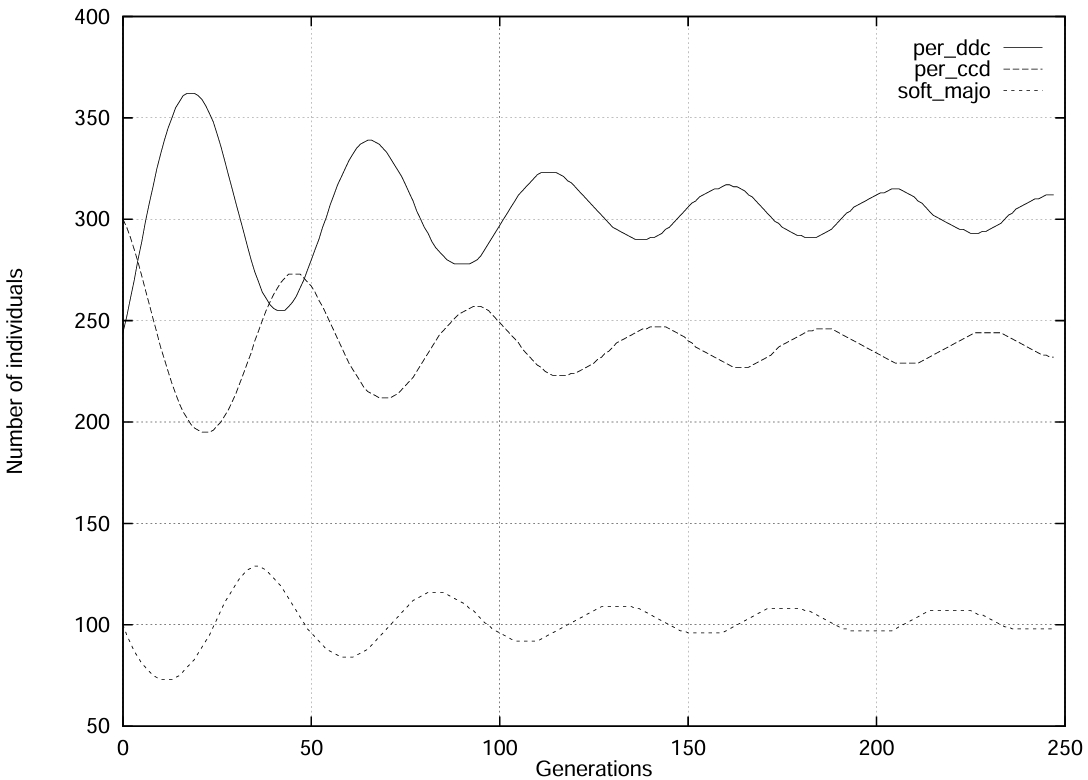
\includegraphics[width=0.7\textwidth]{RefPaperFigures/fig9b.jpeg}\par\vspace{0.5em}
	    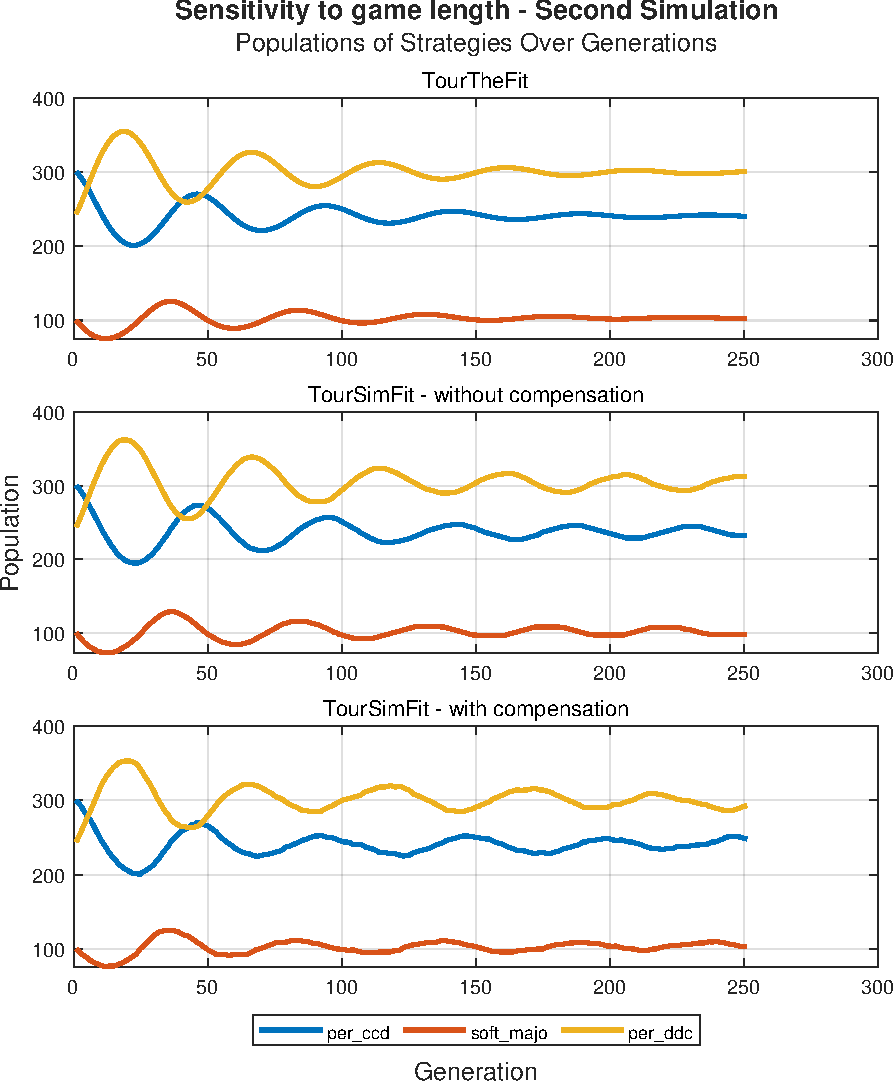
\includegraphics[width=0.7\textwidth]{Sensitivity to game length - Second Simulation.pdf}
	    \caption{12th Simulation - Sensitivity to game length - Second Simulation}
	    \label{fig:Sensitivity to game length - Second Simulation}
	\end{figure}
\subsubsection{13th Simulation - Sensitivity to CIPD payoff - First Simulation}
One other initial condition of the simulation that affects the results greatly is the CIPD payoff, meaning the payoff matrix $B$. This should not come as a surprise; the fitness of each strategy is calculated based on the scores of each match, which in turn is calculated by the payoff matrix. We have also seen in a previous example (Figure~\ref{fig:Increasing oscillations}) how even a slight change to a single element of the payoff matrix can lead to different ensuing dynamics. In the first simulation, the payoff matrix 
\[
B = \begin{bmatrix} 3 & 0 \\ 4.6 & 1 \end{bmatrix}
\] 
is chosen, resulting in increasing oscillations. This is recreated (Figure~\ref{fig:Sensitivity to CIPD payoff - First Simulation}) by all three of the functions, with a slight difference in the cases of TourTheFit and TourSimFit with compensation being that the oscillation ends quicker, as all the members of the population end up using the \texttt{per\_ccd} strategy. Run example13 of the Examples folder (after reading Quickstart guide) to recreate the figure.
	\begin{figure}[h]
	    \centering
		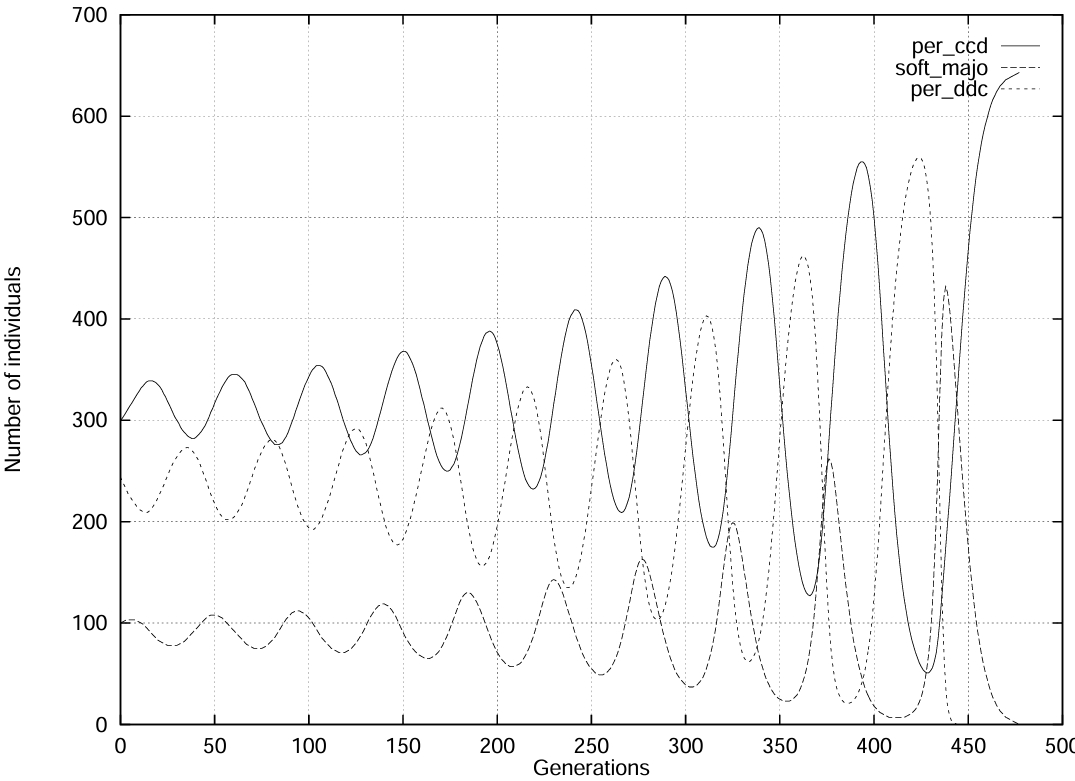
\includegraphics[width=0.7\textwidth]{RefPaperFigures/fig10a.jpeg}\par\vspace{0.5em}
	    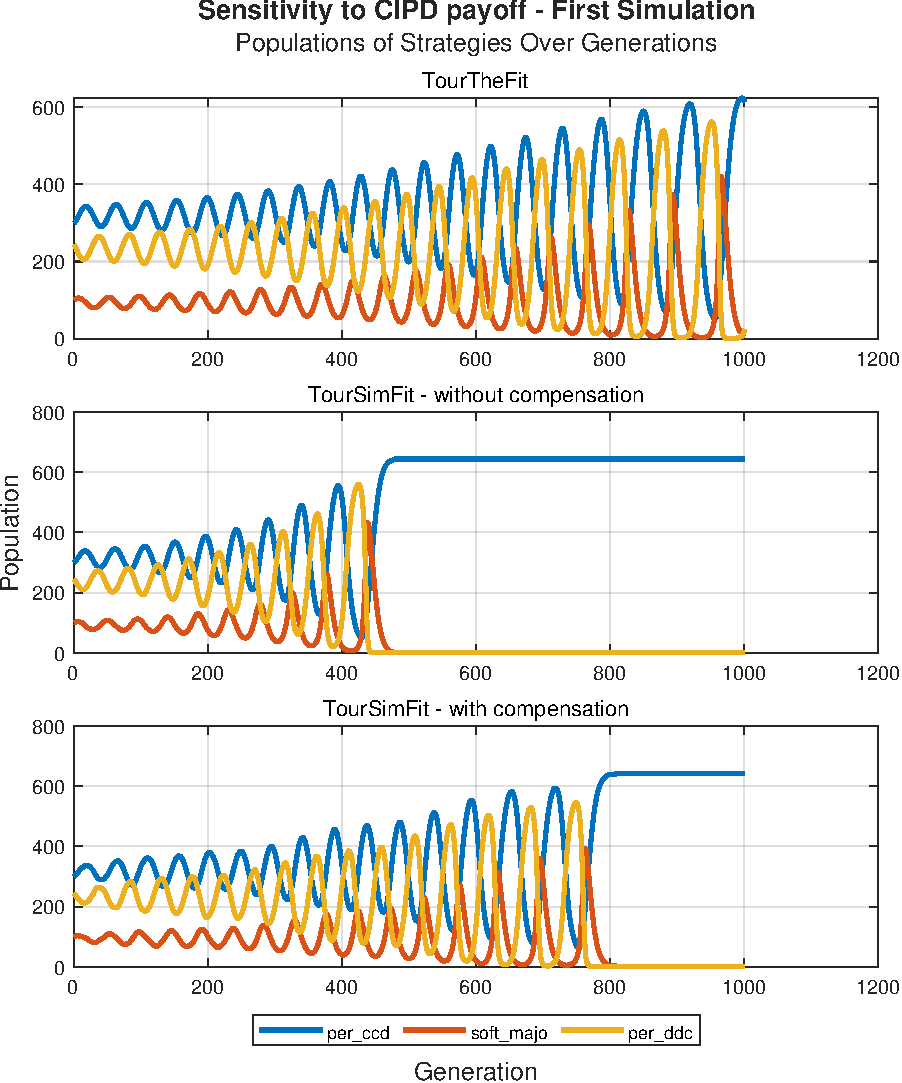
\includegraphics[width=0.7\textwidth]{Sensitivity to CIPD payoff - First Simulation.pdf}
	    \caption{13th Simulation - Sensitivity to CIPD payoff - First Simulation}
	    \label{fig:Sensitivity to CIPD payoff - First Simulation}
	\end{figure}
\subsubsection{14th Simulation - Sensitivity to CIPD payoff - Second Simulation}
In the second part of the comparison the payoff matrix is changed slightly to
\[
B = \begin{bmatrix} 3 & 0 \\ 4.7 & 1 \end{bmatrix}
\] 
resulting in periodic movements. This behavior is also presented by all functions (Figure~\ref{fig:Sensitivity to CIPD payoff - Second Simulation}), thus showing that the payoff matrix is capable of changing the resulting dynamics even with a minor adjustment. Run example14 of the Examples folder (after reading Quickstart guide) to recreate the figure.
	\begin{figure}[h]
	    \centering
		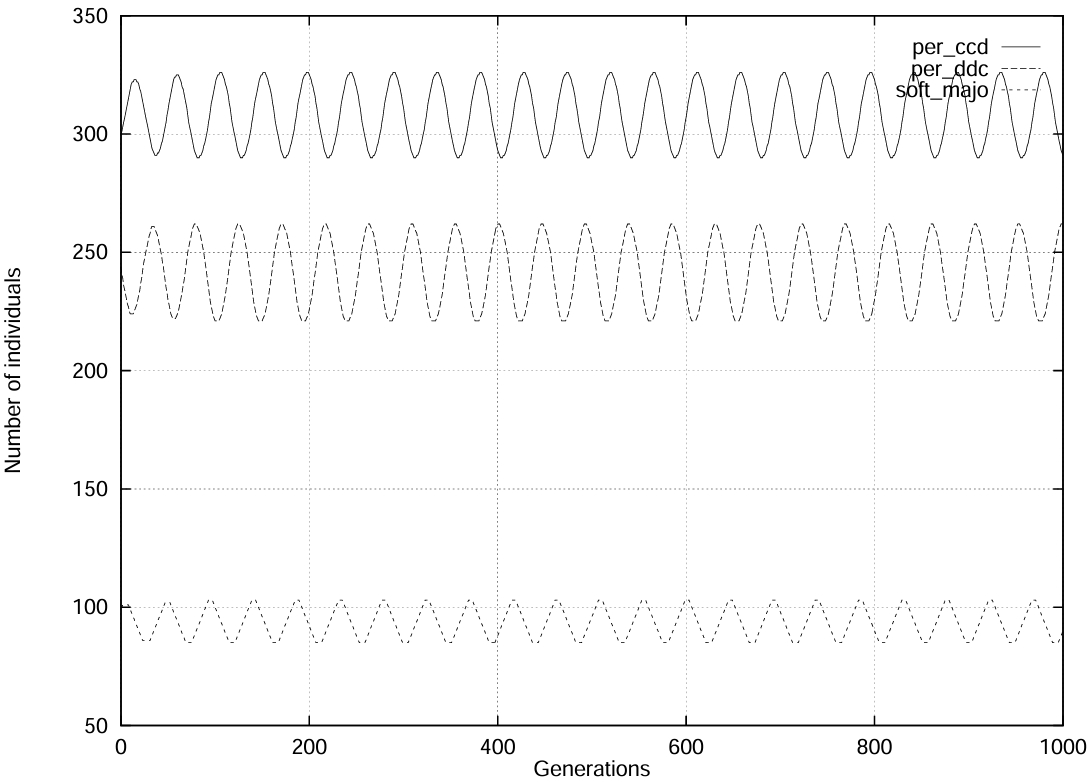
\includegraphics[width=0.7\textwidth]{RefPaperFigures/fig10b.jpeg}\par\vspace{0.5em}
	    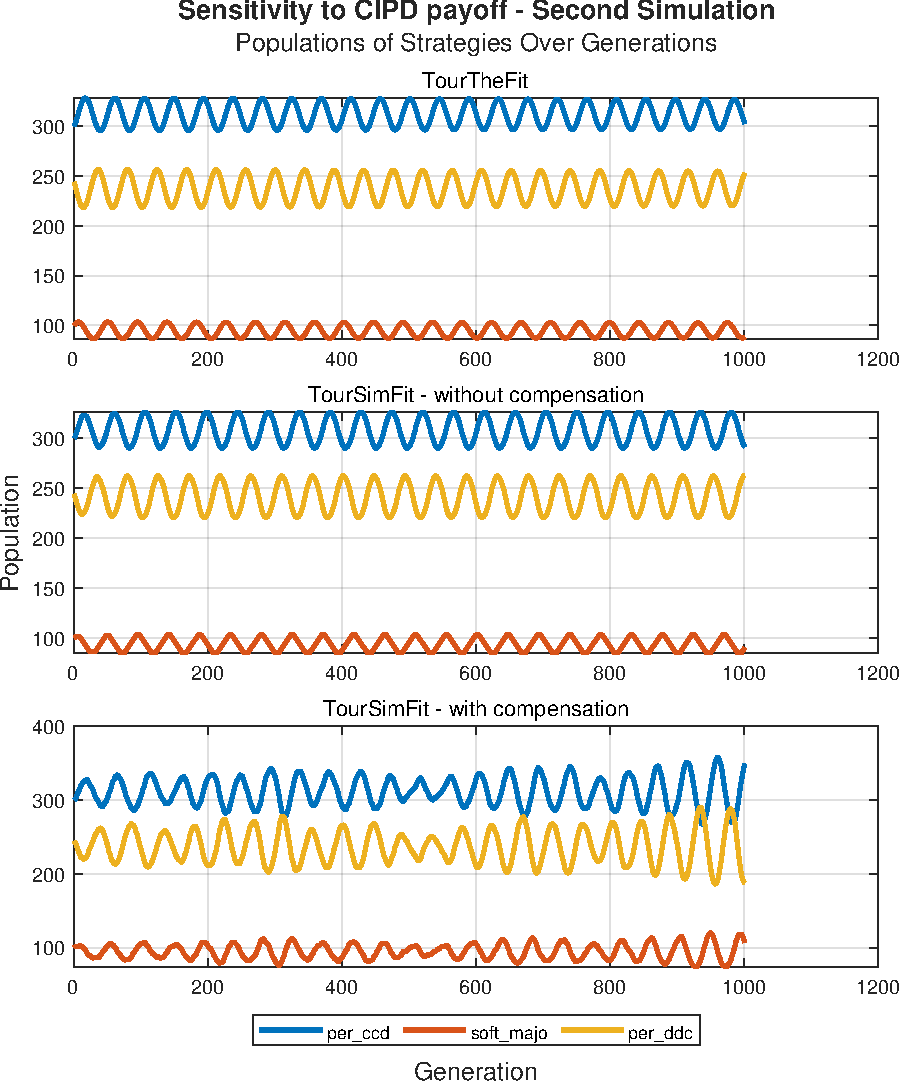
\includegraphics[width=0.7\textwidth]{Sensitivity to CIPD payoff - Second Simulation.pdf}
	    \caption{14th Simulation - Sensitivity to CIPD payoff - Second Simulation}
	    \label{fig:Sensitivity to CIPD payoff - Second Simulation}
	\end{figure}
\subsubsection{15th Simulation - Sensitivity to repartition computation method - First Simulation}
The last aspect of the simulation that is capable of producing vastly different results if altered is the repartition computation method of the simulation, meaning the way the population of the next generation is calculated. This should already be clear, since the functions of the project already have showcased different results in multiple simulations. To start, Mathieu et al calculate the population of the next generation both by rounding to the lower integer and by keeping the float number calculated (thus creating the TourTheFit function). The results are presented in Figure~\ref{fig:Sensitivity to repartition computation method - First Simulation}; the results of the plots by Mathieu et al match the results of TourSimFit with compensation and TourTheFit accordingly. Note that TourSimFit with compensation creates a similar periodic movement to the case without compensation. Also note that both plots presented by Mathieu et al are given in the same figure this time. This happens because the difference being showcased is essentially the difference between TourTheFit and TourSimFit, which we present neatly with our Figure. Run example15 of the Examples folder (after reading Quickstart guide) to recreate the figure.
	\begin{figure}[h]
	    \centering
		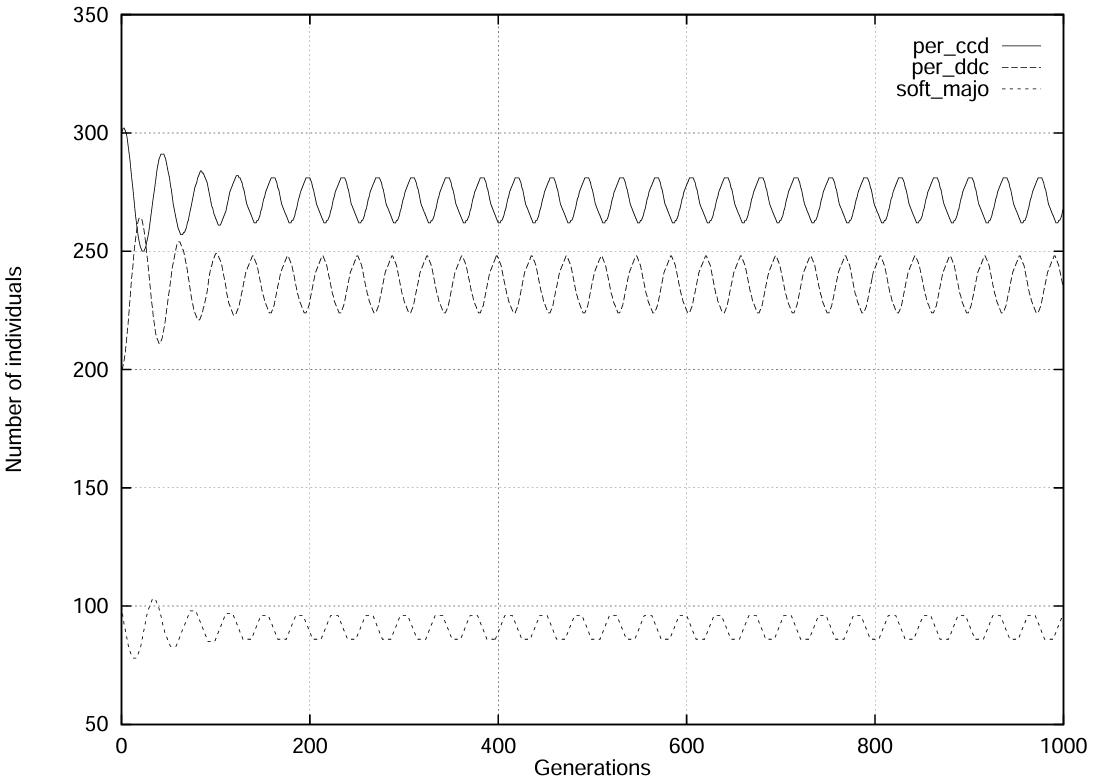
\includegraphics[width=0.49\textwidth]{RefPaperFigures/fig11a.jpeg}
		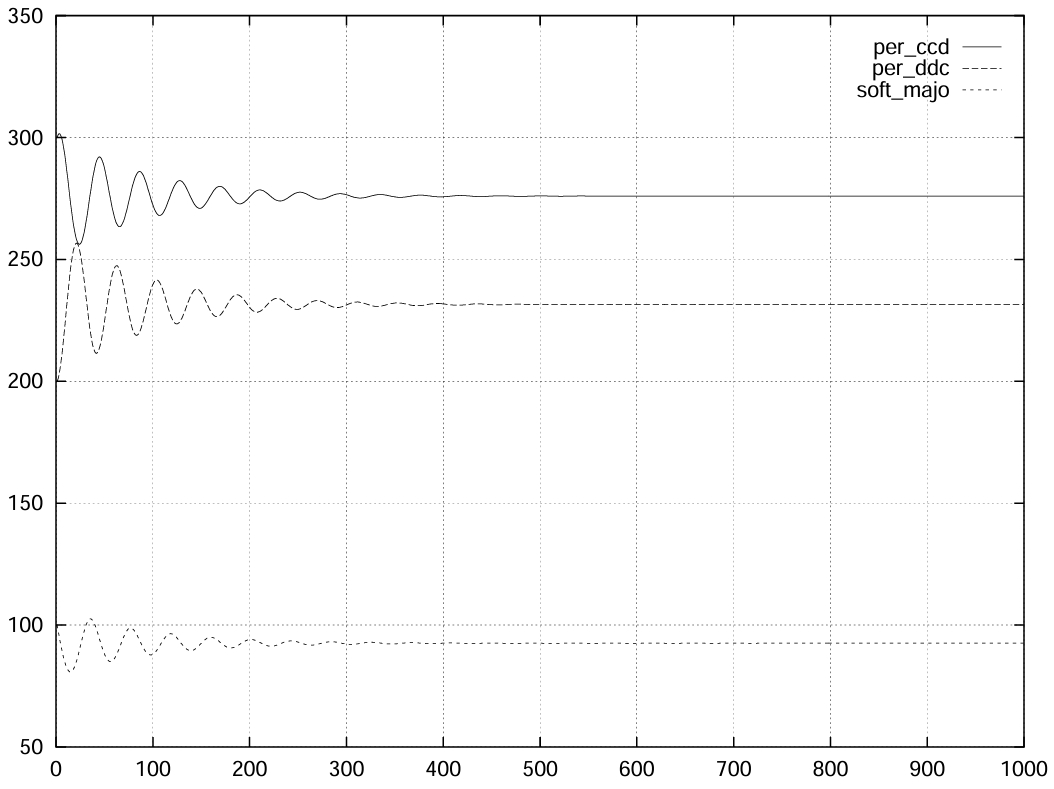
\includegraphics[width=0.49\textwidth]{RefPaperFigures/fig11b.jpeg}\par\vspace{0.5em}\par\vspace{0.5em}
	    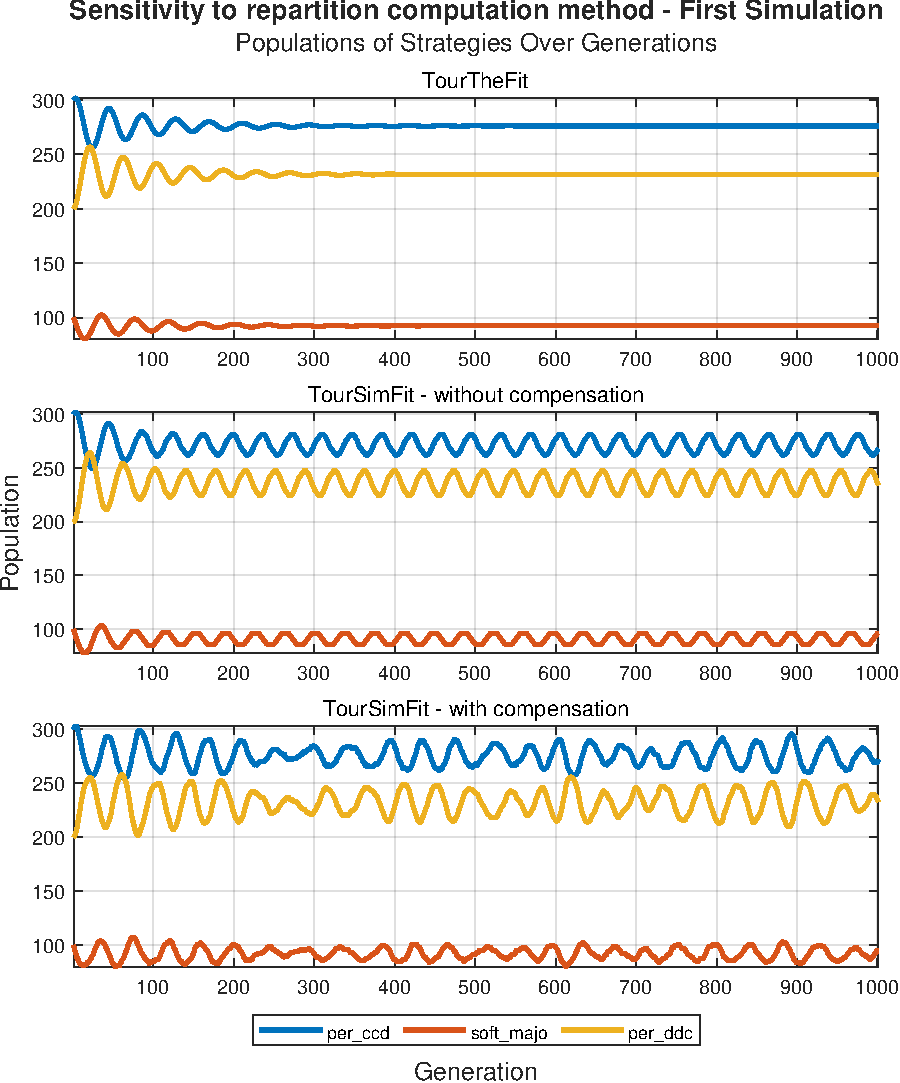
\includegraphics[width=0.7\textwidth]{Sensitivity to repartition computation method - First Simulation.pdf}
	    \caption{15th Simulation - Sensitivity to repartition computation method - First Simulation}
	    \label{fig:Sensitivity to repartition computation method - First Simulation}
	\end{figure}
\subsubsection{16th Simulation - Sensitivity to repartition computation method - Second Simulation}
This final pair of simulations again showcases the sensitivity to the repartition computation method, this time by keeping the ratios between strategies constant but by changing the actual population each strategy initially has. The results (Figure~\ref{fig:Sensitivity to repartition computation method - Second Simulation}) are exactly the same in all cases, also matching the results by Mathieu et al. Run example16 of the Examples folder (after reading Quickstart guide) to recreate the figure.
	\begin{figure}[h]
	    \centering
		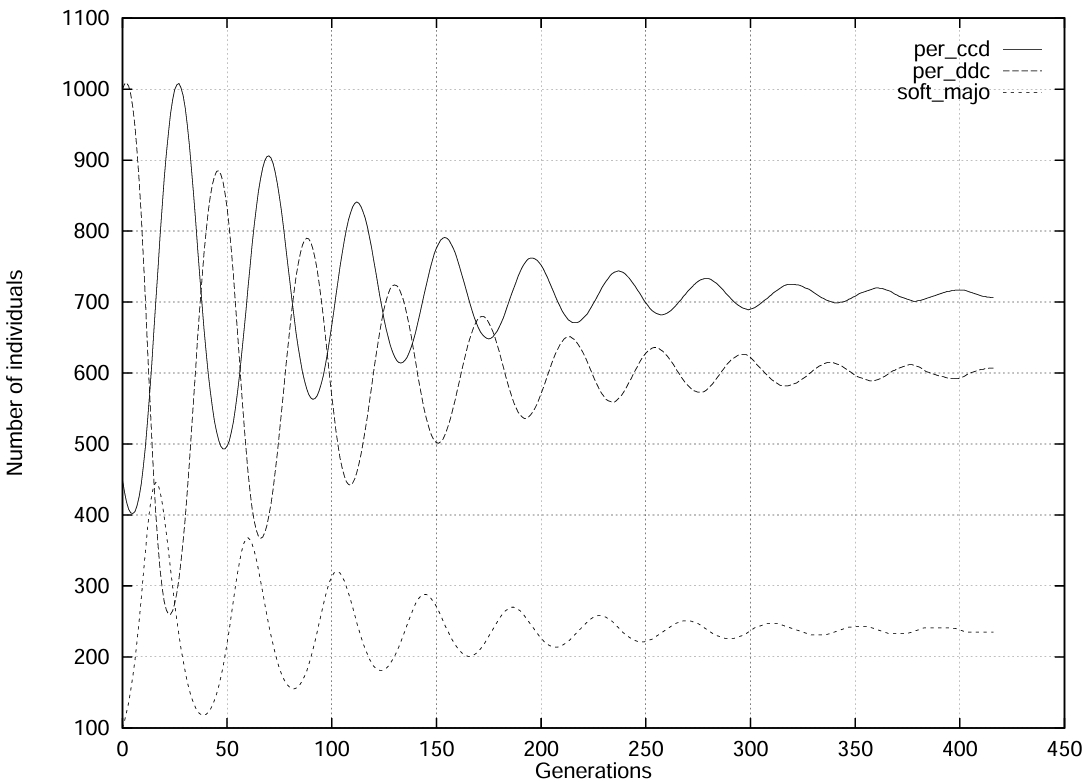
\includegraphics[width=0.7\textwidth]{RefPaperFigures/fig12a.jpeg}\par\vspace{0.5em}
	    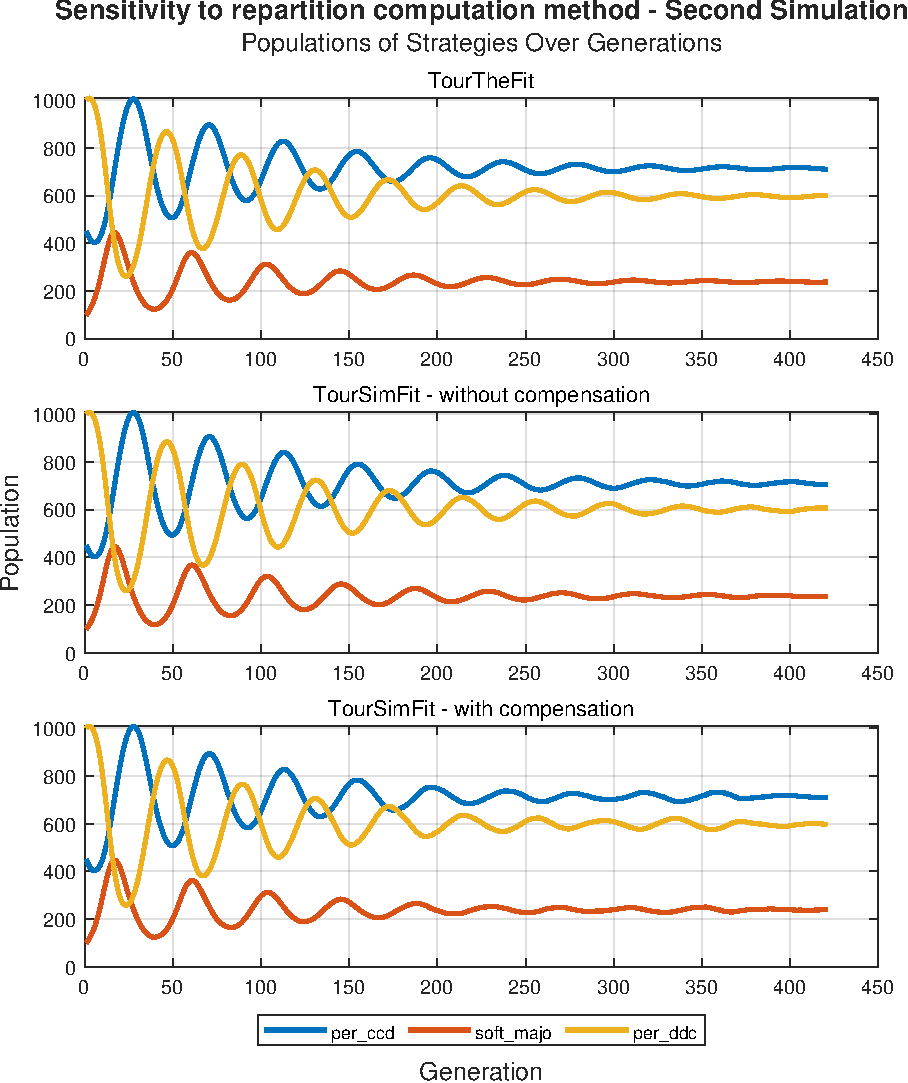
\includegraphics[width=0.7\textwidth]{Sensitivity to repartition computation method - Second Simulation.pdf}
	    \caption{16th Simulation - Sensitivity to repartition computation method - Second Simulation}
	    \label{fig:Sensitivity to repartition computation method - Second Simulation}
	\end{figure}
\subsubsection{17th Simulation - Sensitivity to repartition computation method - Third Simulation}
Lastly, all initial populations of the previous simulation are divided by 10 (thus keeping the ratios of strategies constant). This results in an increasing oscillation in the paper by Mathieu et al. The figure created (Figure~\ref{fig:Sensitivity to repartition computation method - Third Simulation}) shows the same result in the case of TourSimFit wihout compensation, but in the other two cases the dynamics constructed remain attenuated oscillations. Thus, it is once again proven that the method used to calculate the population of the next generation is one of (if not the) most importants aspect in terms of how much the results may differ. Also, it is shown that the ratio between strategies is not always enough to determine the ensuing dynamics; in some cases, such as this, the dynamics are vastly different, just by changing the magnitudes of the populations, not their ratio (from attenuated to increasing oscillations). Run example17 of the Examples folder (after reading Quickstart guide) to recreate the figure.
	\begin{figure}[h]
	    \centering
		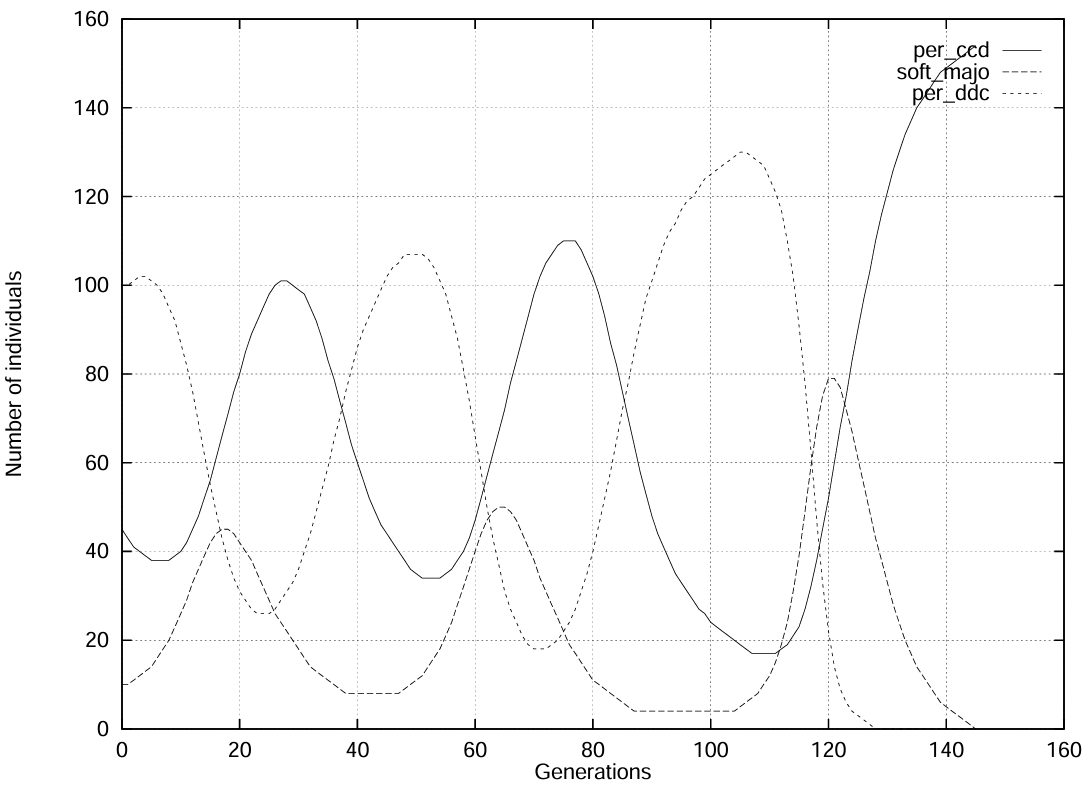
\includegraphics[width=0.7\textwidth]{RefPaperFigures/fig12b.jpeg}\par\vspace{0.5em}
	    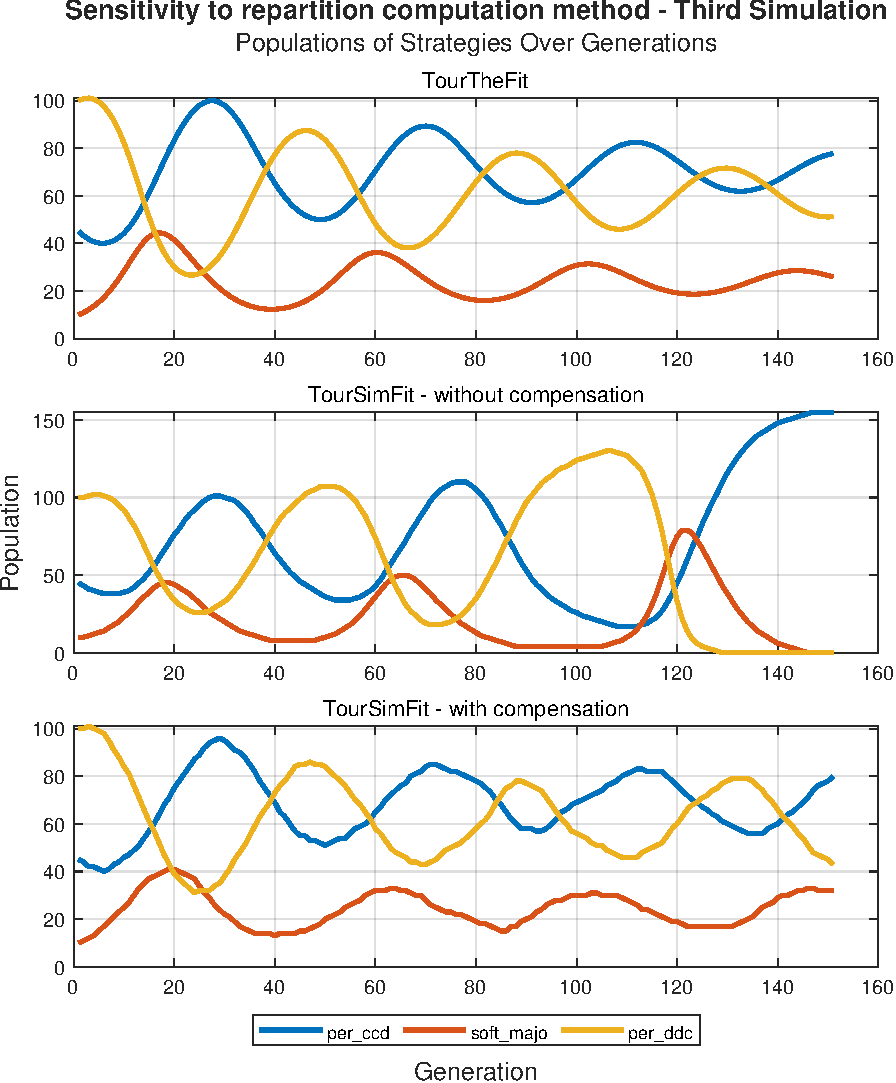
\includegraphics[width=0.7\textwidth]{Sensitivity to repartition computation method - Third Simulation.pdf}
	    \caption{17th Simulation - Sensitivity to repartition computation method - Third Simulation}
	    \label{fig:Sensitivity to repartition computation method - Third Simulation}
	\end{figure}
\subsection{Discussion}

From the above, the following final conclusions emerge regarding the evolutionary \textit{Fitness Dynamics}:

\begin{enumerate}
    \item Mathieu et al.\ appear to have used a simple floor function when calculating new populations after each generation, as this method yielded results closest to ours.

    \item In many cases of generally unstable behaviors, the diagrams differ to an observable degree depending on whether the function \texttt{TourTheFit} or the function \texttt{TourSimFit} is used, with or without compensation. This is due to the fact that many of the resulting diagrams are highly sensitive, and even a small change in the dynamics logic can significantly alter the results.

    \item The resulting diagram depends on the initial population values, the strategies used, and the payoff matrix. Even if two of these factors remain the same, a change in one of them can lead to drastically different results (even different rankings, as seen in Figure~\ref{fig:Increasing oscillations}).

    \item Assigning the remaining population members randomly according to the logic of compensation seems to be a good choice, especially given its simplicity, as it does not significantly alter the results (strategies that theoretically die out actually do die out; in general, the population tendencies do not change). Depending on the specific case being examined, it resembles either the \texttt{TourTheFit} case or the \texttt{TourSimFit} case without compensation.

    \item In general, the discrete nature of the \texttt{TourSimFit} simulations, with or without compensation, leads over time either to recurring oscillations or convergence to certain final population values. Chaos cannot really be achieved; even in Figure~\ref{fig:Disordered oscillations}, the populations eventually converge to the values predicted by \texttt{TourTheFit}. However, this does not prevent us from generating the interesting results seen in the paper.
    
    \item The results depend on many factors including the game length, the payoff matrix, the initial population (both ratio and magnitude) and the repartition computation method.
\end{enumerate} % Include the Fitness Dynamics chapter
\section{Imitation Dynamics}
The second evolutionary dynamic to be presented is that of \textit{Imitation Dynamics}. In this case, the new distribution of the population is not calculated strictly as a function of the fitness of each strategy for each generation. Instead, a simpler and perhaps more realistic logic is adopted: in each generation, we identify the strategy (or, in case of a tie, the strategies) that performed best. Then, given a defined number \( K \) of players who change strategy per generation, \( K \) non-optimal strategy players are randomly selected and each adopts one of the optimal strategies, again randomly, in the case of ties.

It is important to highlight that the selection is only made among players who are not already using an optimal strategy, and not among all players in the population. We consider this to reflect reality more accurately --- if a player is already following an optimal strategy, why would they consider changing? This choice has some consequences on the results that are presented below.

To determine the optimal strategy, a score calculation similar to that used in the fitness dynamics case is employed, in order to save computational time. That is, matches between every player are not actually simulated; instead, scores are calculated based on the payoffs of each strategy against each other strategy and the corresponding population sizes.

As will be shown below during the theoretical presentation of the \texttt{TourTheImi} function, this process can be formulated using a Markov chain, where the states are the various possible population distributions, based on the sum of the initial populations (the total population) and the number of strategies involved in the process. The theoretical background is crucial to understand the following implementations: initially, we consider the \( r \)-state Markov chain, where each state represents the individual strategy of each player. For example, for \( N = 5 \) players and 3 strategies, a possible \( r \)-state is (11323). We then consider the \( s \)-states, where a state represents the population of each strategy; in the previous example, the \( s \)-state would be (212). Essentially, this involves grouping various \( r \)-states into one \( s \)-state, which, since we are not truly interested in each individual player but in the total population per strategy, is equivalent. It is shown that the process \( r(t) \) is lumpable and therefore that \( s(t) \) is a Markov chain. This theoretical knowledge is necessary for the implementation of \texttt{TourTheImi} below.

\subsection{The function TourSimImi}
The function that simulates the evolutionary tournament with imitation dynamics is implemented as
\[
[\text{POP}, \text{BST}] = \text{TourSimImi}(B, \text{Strategies}, \text{POP}_0, K, T, J, \text{mode}).
\]
The inputs and outputs of the function are similar to those of \texttt{TourSimFit}, with the additional argument \( K \), an integer value that specifies the number of players who change strategy per generation. The additional argument \texttt{mode} (the function runs with default value \texttt{"Individual"}) can take the values \texttt{"Individual"} and \texttt{"Total"}, and refers to the way in which the optimal strategy is selected: in the \texttt{"Individual"} case, the strategy of the best individual player is returned, while in the \texttt{"Total"} case, the strategy with the highest total score among the players using it is selected. The choice of mode yields significantly different results, as will be shown below.

\subsection{The function TourTheImi}
The \texttt{TourTheImi} function has the form
\[
P = \text{TourTheImi}(B, \text{Strategies}, \text{POP}_0, K, T, J, \text{mode})
\]
with arguments identical to the function \texttt{TourSimImi}, and output the transition matrix \( P \) of the Markov chain of the s-states. In reality, the initial population is used only to determine the total population size of the tournament (so it could simply be replaced by an argument \( N \)), and the number of generations \( J \) is not used at all.

For this analysis, we consider the s-states of the tournament as the number of players using each strategy. For example, for \( N = 9 \), we may have
\[
s_1 = \begin{bmatrix} 0 & 0 & 9 \end{bmatrix}, \quad s_2 = \begin{bmatrix} 0 & 1 & 8 \end{bmatrix},
\]
and so on. Depending on the \texttt{mode} argument, we expect the transition matrix to take different forms. For example, in \texttt{"Individual"} mode and with strategies \texttt{All\_D}, \texttt{All\_C}, and \texttt{TitForTat}, we expect the state
\[
\begin{bmatrix} 0 & 5 & 4 \end{bmatrix}
\]
to be absorbing, since there are no non-optimal players, and therefore it should have only one transition — to itself — with probability 1. In contrast, in the \texttt{"Total"} mode, this state would not be absorbing, as the \texttt{All\_C} strategy accumulates more total points.

Another function is also created:
\[
\text{AnalyzeMarkovChain}(P, \text{POP}_0, \text{Strategies}, \text{Title}),
\]
which is responsible for generating the state transition diagrams shown below. This function, based on the matrix \( P \) calculated by the \texttt{TourTheImi} function and the initial population \texttt{POP0}, classifies the states into transient, absorbing, and the initial state. It also further distinguishes between reachable and unreachable states based on the initial state. It generates a diagram of each state, where the state type is indicated with color, the population of each strategy is shown, the strategy names are labeled (as given by the \texttt{Strategies} argument), and the corresponding transition probabilities are displayed above each transition. The \texttt{Title} argument is the title of the resulting diagram.

\subsection{Simulations - Examples}
Παρακάτω παρουσιάζονται κάποιες προσομοιώσεις οι οποίες παράγονται από τις συναρτήσεις που περιγράφηκαν παραπάνω και παρουσιάζουν ενδιαφέρον. Η κάθε προσομοίωση βρίσκεται στο αρχείο example.m σε κατάλληλο Section και με Run Section προκύπτουν ακριβώς τα αποτελέσματα που παρουσιάζονται παρακάτω.
\subsubsection{1η Προσομοίωση - Παράδειγμα χρήσης των Tour\-The\-Imi, Analyze\-Markov\-Chain και Tour\-Sim\-Imi}
Στην πρώτη προσομοίωση \ref{fig:TourTheImi153} παρουσιάζεται η μαρκοβιανή αλυσίδα που προκύπτει για τις στρατηγικές $\begin{bmatrix}All\_D&All\_C&TitForTat\end{bmatrix}$ σε μείγμα $\begin{bmatrix}1&5&3\end{bmatrix}$.
Από το διάγραμμα που προκύπτει παρατηρούμε ότι οι πιθανές απορροφητικές καταστάσεις είναι η $\begin{bmatrix}9&0&0\end{bmatrix}$, δηλαδή η επικράτηση της στρατηγικής $All\_D$, η $\begin{bmatrix}0&0&9\end{bmatrix}$, δηλαδή η επικράτηση της στρατηγικής $TitForTat$ και η $\begin{bmatrix}0&1&8\end{bmatrix}$, δηλαδή η επικράτηση της $TitForTat$ αλλά με επιβίωση της $All\_C$. Από τις πιθανότητες μετάβασης, που απεικονίζονται στα βέλη των μεταβάσεων, παρατηρούμε ότι η τελευταία απορροφητική κατάσταση έχει σημαντικά χαμηλότερη πιθανότητα να συμβεί σε σχέση με τις άλλες δύο. Ακόμη παρατηρούμε ότι οι καταστάσεις στις οποίες υπάρχουν μόνο οι συμπαθείς στρατηγικές ($All\_C$ και $TitForTat$), δηλαδή στρατηγικές οι οποίες ποτέ δεν λιποτακτούν πρώτες και άρα οι παίκτες των οποίων αποκτούν ίσα σκορ παίζοντας μεταξύ τους, μεταβαίνουν μόνο στον εαυτό τους καθώς δεν υπάρχουν παίκτες με σκορ χαμηλότερο του μεγίστου.

	\begin{figure}[h]
	      \centering
	      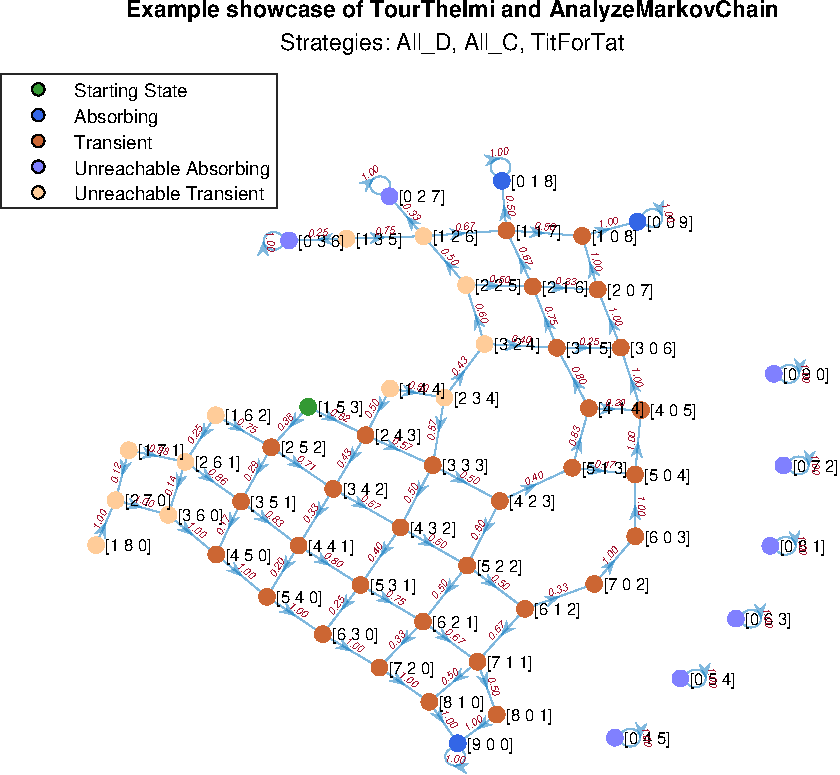
\includegraphics[width=0.95\textwidth]{Example showcase of TourTheImi and AnalyzeMarkovChain.pdf}
	      \caption{Example showcase of TourTheImi and AnalyzeMarkovChain}
	      \label{fig:TourTheImi153}
	\end{figure}
	
Στο Σχήμα \ref{fig:TourSimImi153} απεικονίζονται δύο εκτελέσεις της TourSimImi για το μείγμα στρατηγικών της παραπάνω προσομοίωσης. Παρατηρούμε ότι λόγω του τυχαίου τρόπου επιλογής των imitators, δηλαδή των παικτών που δεν έχουν την καλύτερη στρατηγική και αλλάζουν σε κάποια από τις καλύτερες, το τελικό μείγμα στρατηγικών είναι διαφορετικό για κάθε εκτέλεση του προγράμματος. Συγκεκριμένα στην (α) εκτέλεση παρατηρούμε $\begin{bmatrix}1&5&3\end{bmatrix} \rightarrow^* \begin{bmatrix}9&0&0\end{bmatrix}$ ενώ στην (β) εκτέλεση $\begin{bmatrix}1&5&3\end{bmatrix} \rightarrow^*	\begin{bmatrix}0&0&9\end{bmatrix}$, που όπως αναλύσαμε παραπάνω είναι πράγματι οι δύο πιο πιθανές απορροφητικές καταστάσεις.
	\begin{figure}[h]
		\centering
		\begin{subfigure}{.5\textwidth}
			\centering
	      	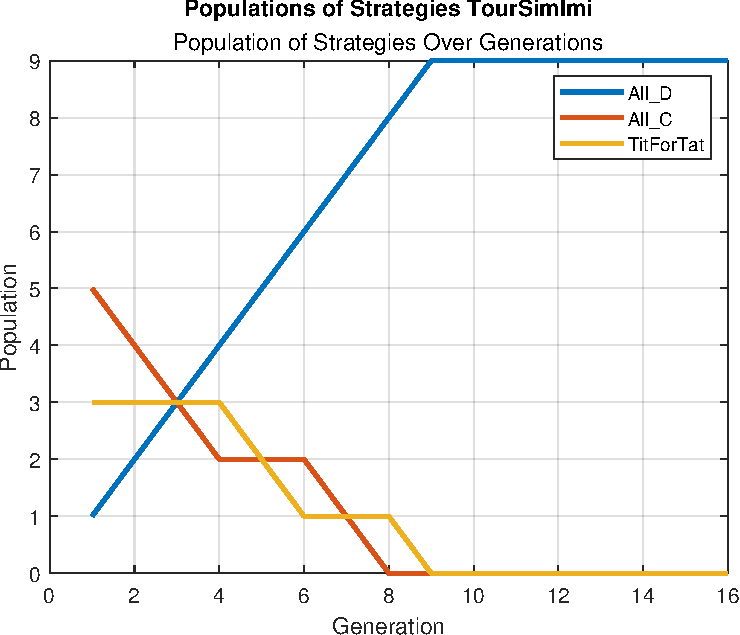
\includegraphics[width=.9\textwidth]{900.pdf}
			\caption{$\begin{bmatrix}9&0&0\end{bmatrix}$}
	      	\label{fig:900}
		\end{subfigure}%
		\begin{subfigure}{.5\textwidth}
			\centering
	      	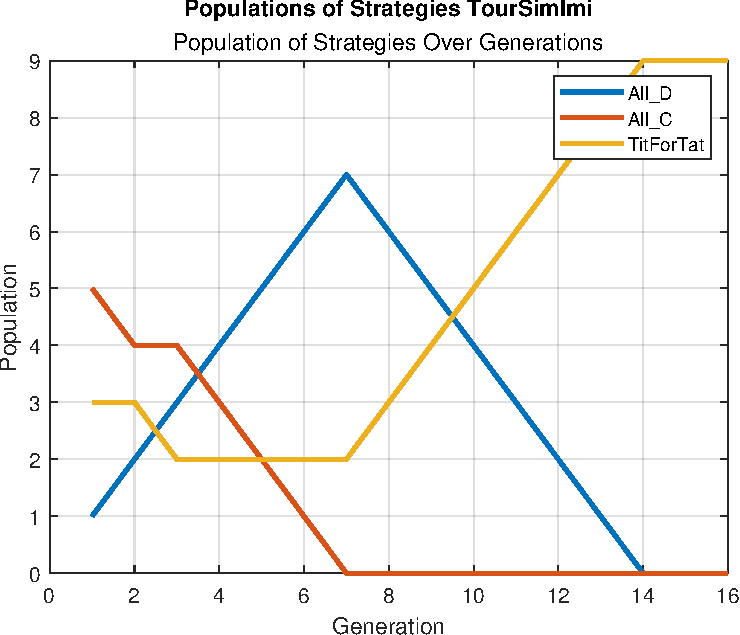
\includegraphics[width=0.90\textwidth]{009.pdf}
			\caption{$\begin{bmatrix}0&0&9\end{bmatrix}$}
	      	\label{fig:009}
		\end{subfigure}
		\caption{Absorbing States may differ even for the same Starting State}
		\label{fig:TourSimImi153}
	\end{figure}

\subsubsection{2η Προσομοίωση - Δοκιμή προεπιλεγμένης μεθόδου (Individual) για τον προσδιορισμό της καλύτερης στρατηγικής}
Στις δύο επόμενες προσομοιώσεις επιχειρείται να παρουσιαστεί η διαφορά στα αποτελέσματα που προκαλεί η διαφορετική μεθοδολογία επιλογής της καλύτερης στρατηγικής. Αρχικά (\ref{fig:TourTheImiIndividual}) παρουσιάζεται η μαρκοβιανή αλυσίδα που προκύπτει για αρχικό μείγμα στρατηγικών $\begin{bmatrix}1&4&5\end{bmatrix}$ και επιλογή μεθόδου ``Individual'', δηλαδή επιλογή της καλύτερης στατηγικής με σύγκριση των payoffs των στρατηγικών με παιχνίδια ένας εναντίον ενός για κάθε ζεύγος στρατηγικών.

Το αποτέλεσμα είναι αντίστοιχο αυτού της πρώτης προσομοίωσης \ref{fig:TourTheImi153}. Με λίγη παρατήρηση μπορούμε να οραματιστούμε μία νοητή καμπύλη μεταξύ των κορυφών των καταστάσεων $\begin{bmatrix}8&0&2\end{bmatrix}, \begin{bmatrix}6&1&3\end{bmatrix}, \begin{bmatrix}4&2&4\end{bmatrix}, \begin{bmatrix}2&3&5\end{bmatrix}$ η οποία χωρίζει τις λεκάνες απορροής των συμπαθών και των μη-συμπαθών στρατηγικών. Αν βρεθούμε σε κατάσταση κάτω από αυτή την καμπύλη θα καταλήξουμε στην απορροφητική κατάσταση επικράτησης της ``All\_D'', ενώ από κατάσταση πάνω από αυτή την καμπύλη θα καταλήξουμε σε μία από τις απορροφητικές καταστάσεις των συμπαθών στρατηγικών.
	\begin{figure}[h]
	      \centering
	      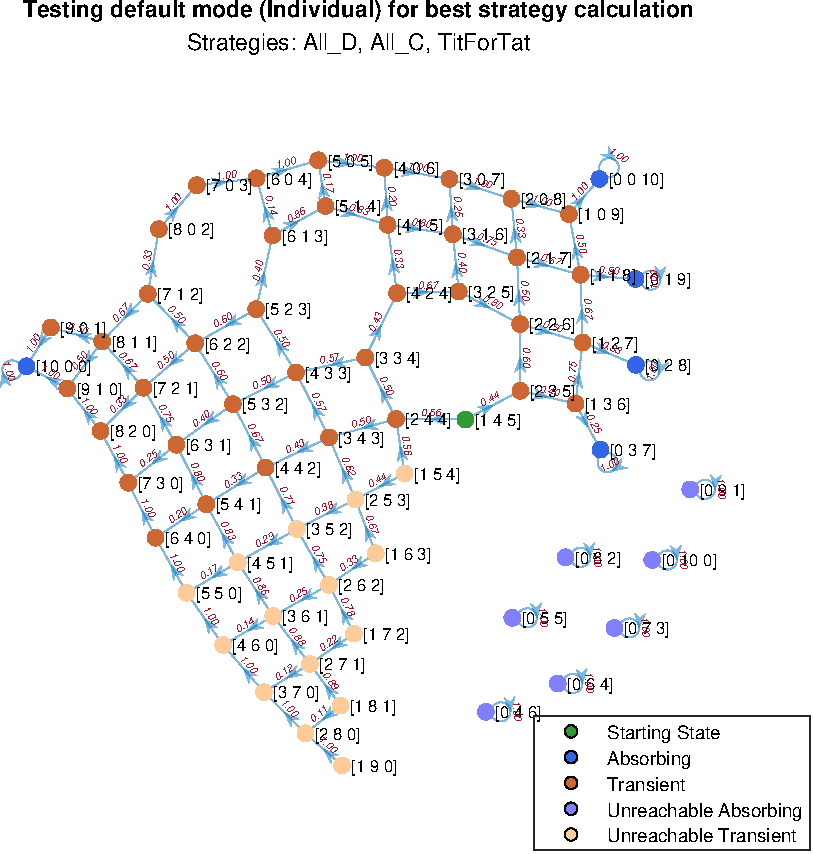
\includegraphics[width=0.95\textwidth]{Testing default mode (Individual) for best strategy calculation.pdf}
	      \caption{Testing default mode (``Individual'') for best strategy calculation with $POP0=\begin{bmatrix}1&4&5\end{bmatrix}$}
	      \label{fig:TourTheImiIndividual}
	\end{figure}
\subsubsection{3η Προσομοίωση - Δοκιμή μεθόδου ``Total'' για τον προσδιορισμό της καλύτερης στρατηγικής}
Στην τρίτη προσομοίωση (\ref{fig:TourTheImiTotal}) για ίδιο αρχικό μείγμα στρατηγικών $\begin{bmatrix}1&4&5\end{bmatrix}$ και επιλογή μεθόδου ``Total'', δηλαδή σύγκριση των payoffs των παικτών που προκύπτουν σε κάθε state από Axelrod με τους πληθυσμούς του state και επιλογή ως καλύτερη στρατηγική της στρατηγικής του παίκτη με το μεγαλύτερο συνολικό payoff.

Σε αντίθεση με την προηγούμενη προσομοίωση (\ref{fig:TourTheImiIndividual}) εδώ παρατηρούμε ότι το διάγραμμα είναι χωρισμένο σε τρεις ξεχωριστούς υπογράφους.
Ο πρώτος υπογράφος, αυτός που περιλαμβάνει την αρχική κατάσταση, είναι ο μόνος που περιλαμβάνει προσεγγίσιμη απορροφητική κατάσταση (την $\begin{bmatrix}0&0&10\end{bmatrix}$), η οποία είναι η επικράτηση της ``TitForTat''. Αυτό συμβαίνει διότι κατά την εύρεση της καλυτερης στρατηγικής στο mode ``Total'' οι συμπαθείς στρατηγικές συνεργάζονται μεταξύ τους και υπερνικούν λόγω του μεγαλύτερου πλήθους τους το προβάδισμα που δίνει η λιποταξία στην ``All\_D''
Ο δεύτερος υπογράφος είναι αυτός που περιλαμβάνει την απορροφητική κατάσταση που επικρατεί η ``All\_D'' ($\begin{bmatrix}10&0&0\end{bmatrix}$), η οποία όμως είναι μη προσπελάσιμη όπως και οι μεταβατικές καταστάσεις όλου του υπογράφου, για τον λόγο που περιγράφηκε παραπάνω.
Τέλος ο τρίτος υπογράφος είναι αυτός που περιλαμβάνει την απορροφητική κατάσταση που επικρατεί η ``All\_C'' ($\begin{bmatrix}0&10&0\end{bmatrix}$), η οποία είναι επίσης μη προσπελάσιμη όπως και οι μεταβατικές καταστάσεις όλου του υπογράφου, για τον λόγο που περιγράφηκε παραπάνω.

	\begin{figure}[h]
	      \centering
	      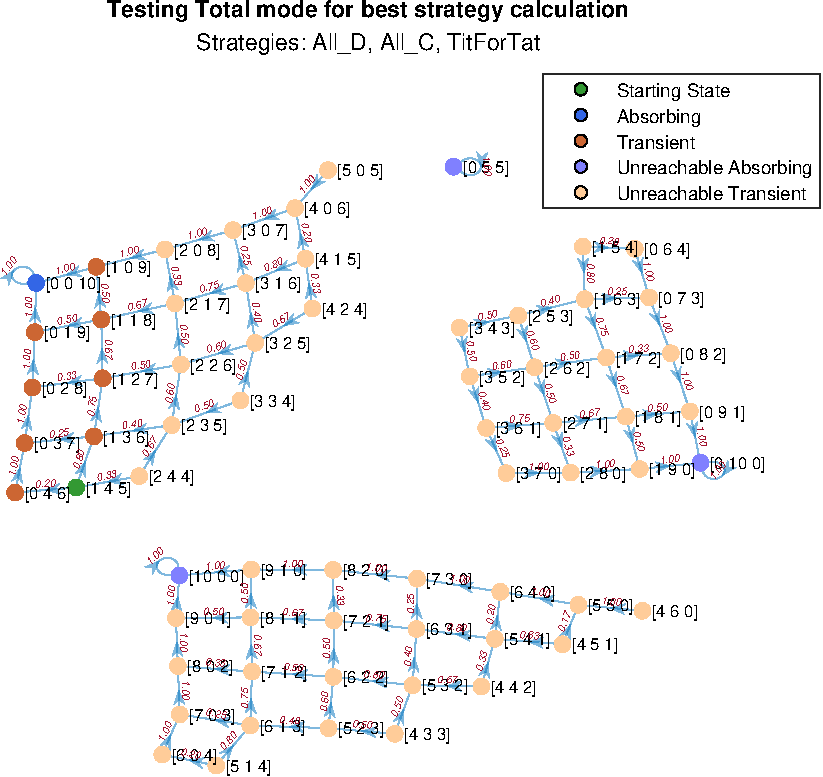
\includegraphics[width=0.95\textwidth]{Testing Total mode for best strategy calculation}
	      \caption{Testing ``Total'' mode for best strategy calculation with $POP0=\begin{bmatrix}1&4&5\end{bmatrix}$}
	      \label{fig:TourTheImiTotal}
	\end{figure}
	
	\begin{figure}[h]
		\centering
		\begin{subfigure}[t]{.49\textwidth}
			\centering
			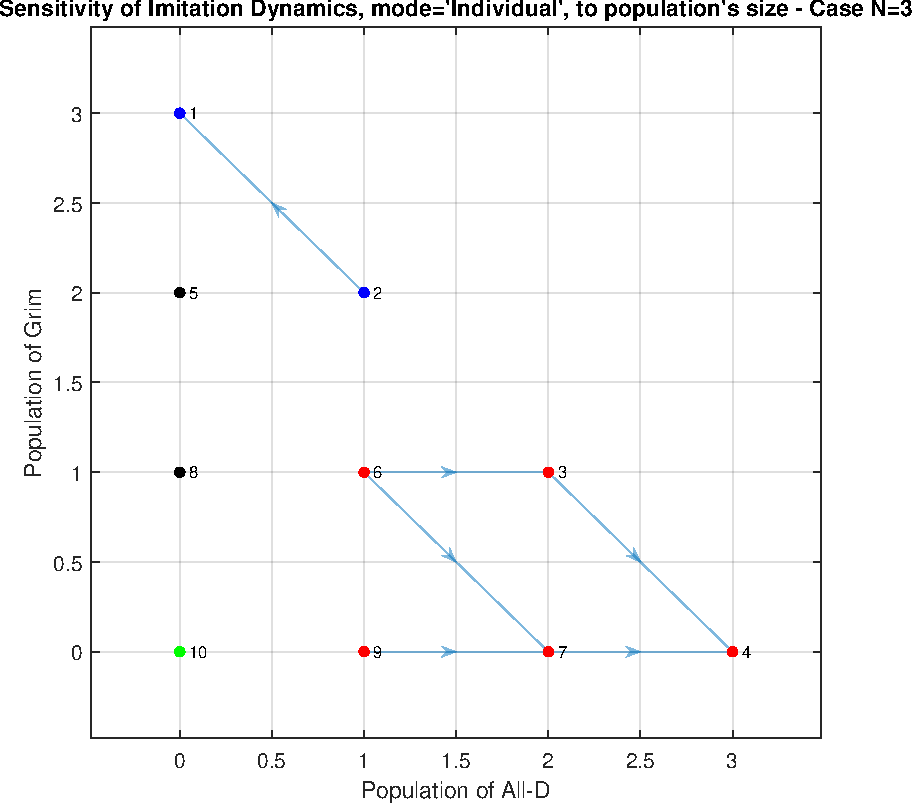
\includegraphics[height=0.8\textwidth]{Sensitivity of Imitation Dynamics, mode='Individual', to population's size - Case N=3}
			\caption{Case $N=3$}
			\label{fig:example18}
		\end{subfigure}
		\begin{subfigure}[t]{.49\textwidth}
			\centering
			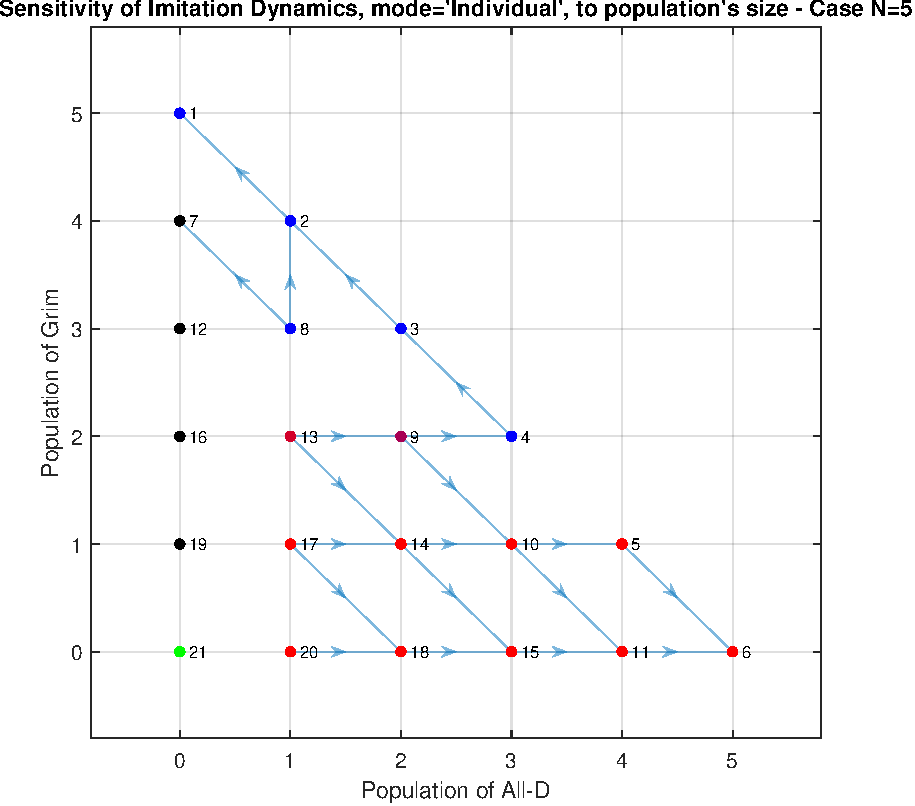
\includegraphics[height=0.8\textwidth]{Sensitivity of Imitation Dynamics, mode='Individual', to population's size - Case N=5}
			\caption{Case $N=5$}
			\label{fig:example19}
		\end{subfigure}
		\par\vspace{1em}
		\begin{subfigure}[t]{.49\textwidth}
			\centering
			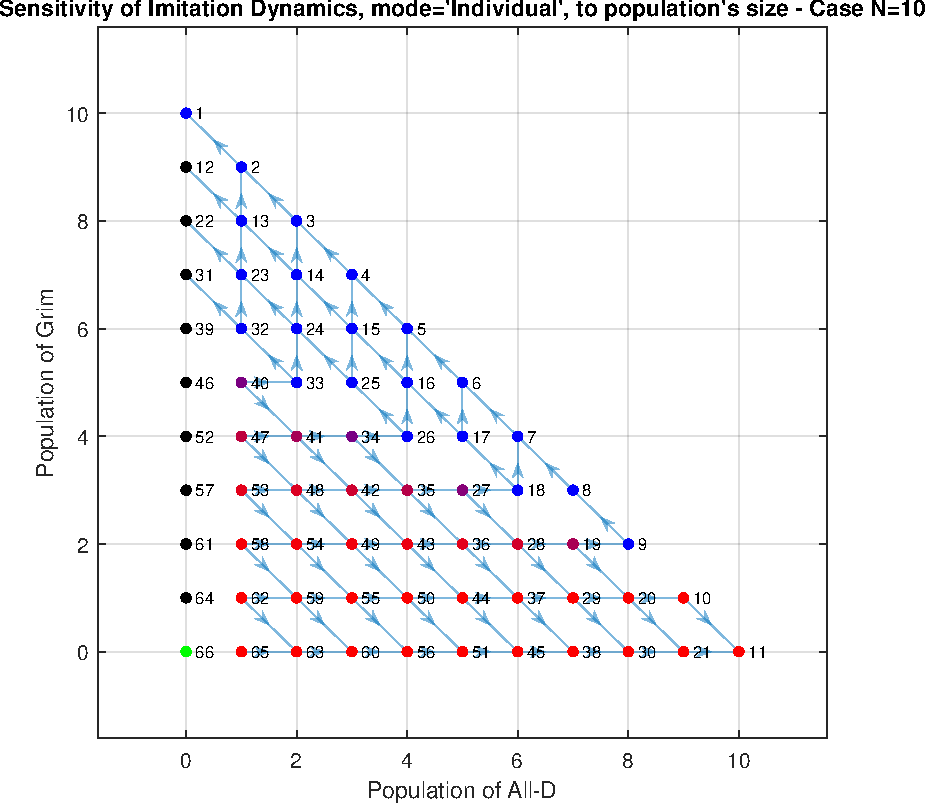
\includegraphics[height=0.8\textwidth]{Sensitivity of Imitation Dynamics, mode='Individual', to population's size - Case N=10}
			\caption{Case $N=10$}
			\label{fig:example20}
		\end{subfigure}
		\begin{subfigure}[t]{.49\textwidth}
			\centering
			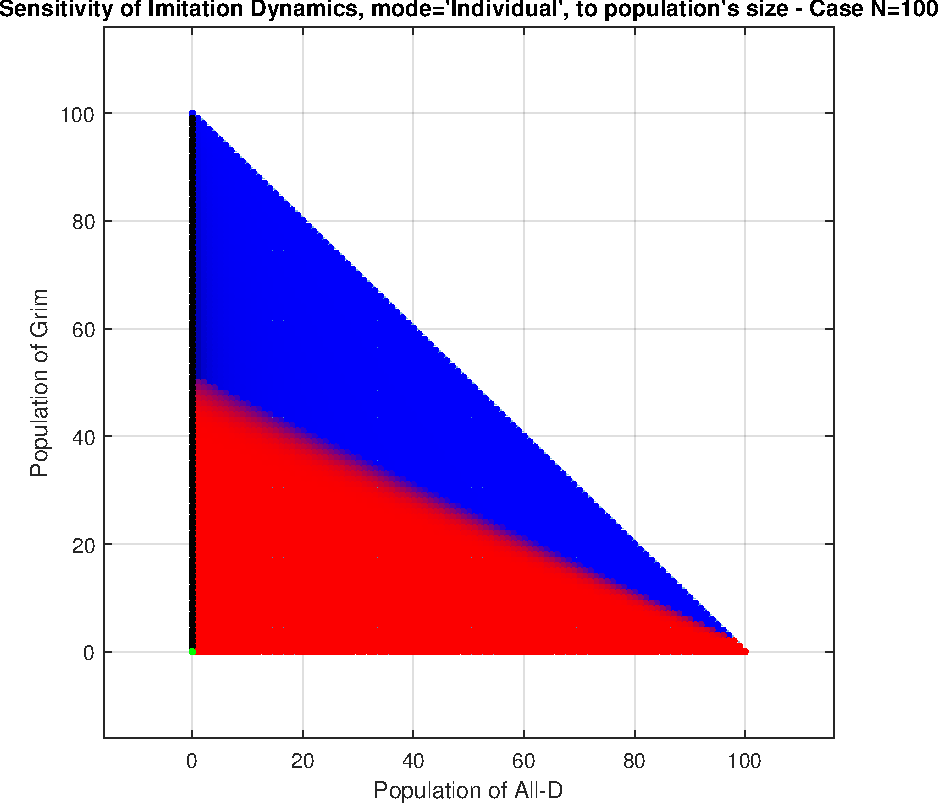
\includegraphics[height=0.8\textwidth]{Sensitivity of Imitation Dynamics, mode='Individual', to population's size - Case N=100}
			\caption{Case $N=100$}
			\label{fig:example21}
		\end{subfigure}
		\caption{Sensitivity of Imitation Dynamics (mode=``Individual'') to population size for $B = \begin{bmatrix} 3 & 1 \\ 4 & 2 \end{bmatrix}$}
		\label{fig:Sensitivity of Imitation Dynamics, mode='Individual', to population's size}
	\end{figure}
	
	\begin{figure}[h]
		\centering
		\begin{subfigure}{.49\textwidth}
			\centering
			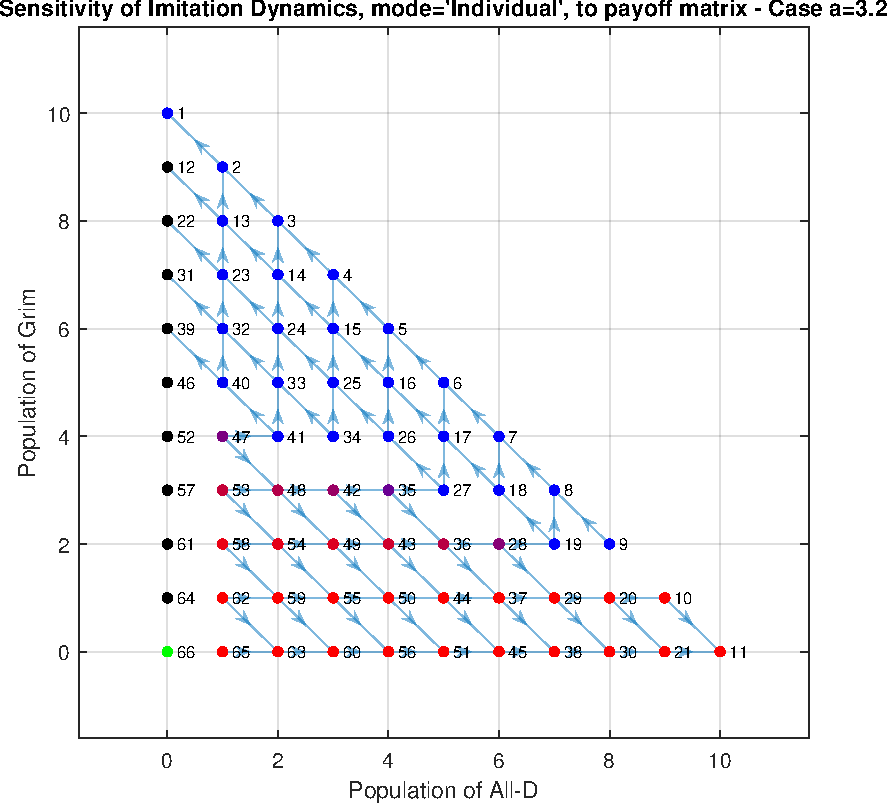
\includegraphics[width=\textwidth]{Sensitivity of Imitation Dynamics, mode='Individual', to payoff matrix - Case a=3.2}
			\caption{Case $a=3.2$}
			\label{fig:example22}
		\end{subfigure}
		\begin{subfigure}{.49\textwidth}
			\centering
			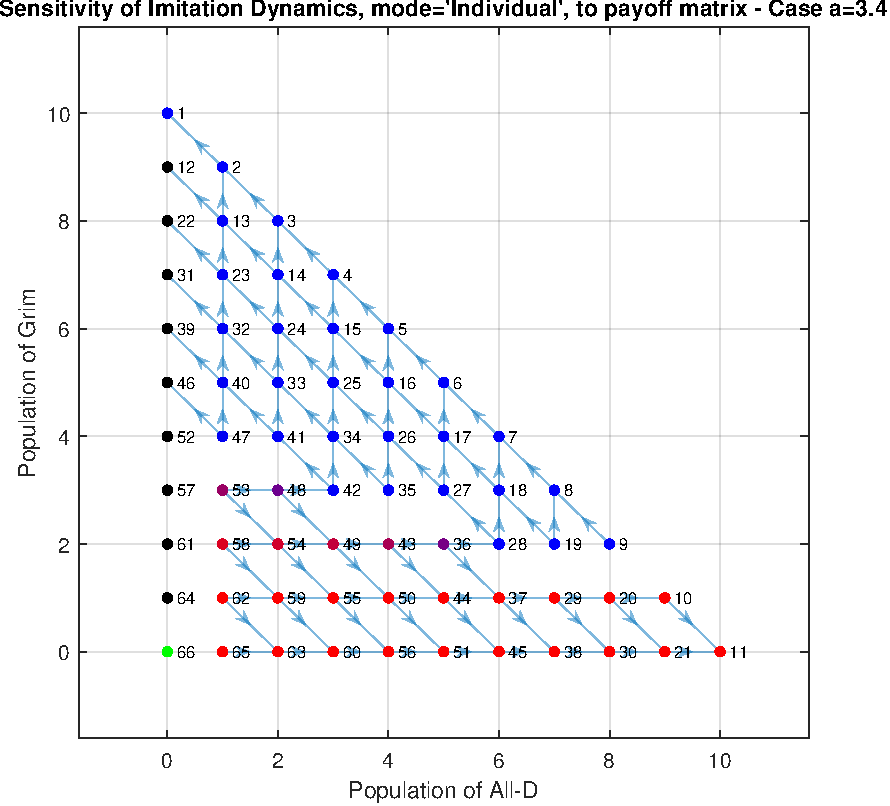
\includegraphics[width=\textwidth]{Sensitivity of Imitation Dynamics, mode='Individual', to payoff matrix - Case a=3.4}
			\caption{Case $a=3.4$}
			\label{fig:example23}
		\end{subfigure}
		\vspace{0.5em}
		\begin{subfigure}{.49\textwidth}
			\centering
			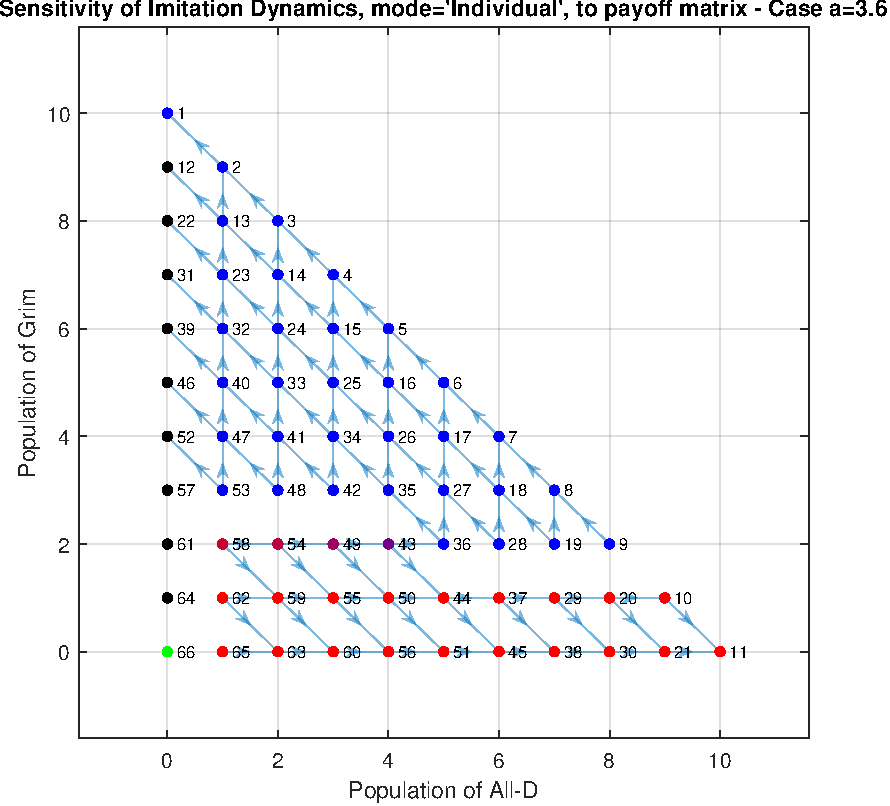
\includegraphics[width=\textwidth]{Sensitivity of Imitation Dynamics, mode='Individual', to payoff matrix - Case a=3.6}
			\caption{Case $a=3.6$}
			\label{fig:example24}
		\end{subfigure}
		\begin{subfigure}{.49\textwidth}
			\centering
			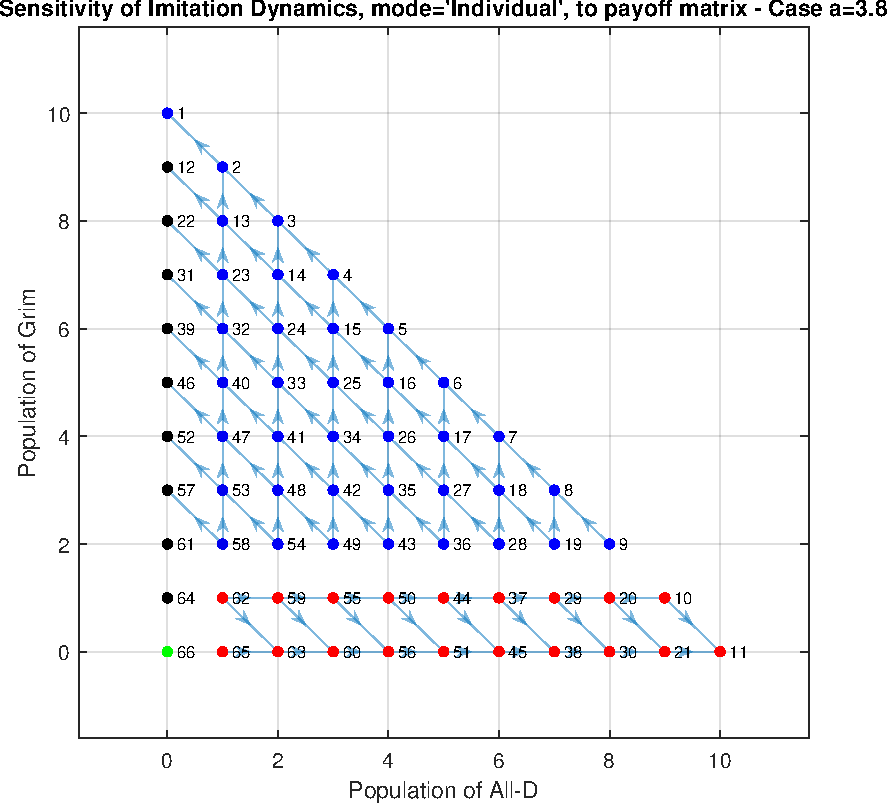
\includegraphics[width=\textwidth]{Sensitivity of Imitation Dynamics, mode='Individual', to payoff matrix - Case a=3.8}
			\caption{Case $a=3.8$}
			\label{fig:example25}
		\end{subfigure}
		\caption{Sensitivity of Imitation Dynamics (mode=``Individual'') to payoff matrix parameter $a$ for $B = \begin{bmatrix} a & 1 \\ 4 & 2 \end{bmatrix}$ and $N=10$}
		\label{fig:Sensitivity of Imitation Dynamics, mode='Individual', to payoff matrix}
	\end{figure}
	
	\begin{figure}[h]
		\centering
		\begin{subfigure}[t]{.49\textwidth}
			\centering
			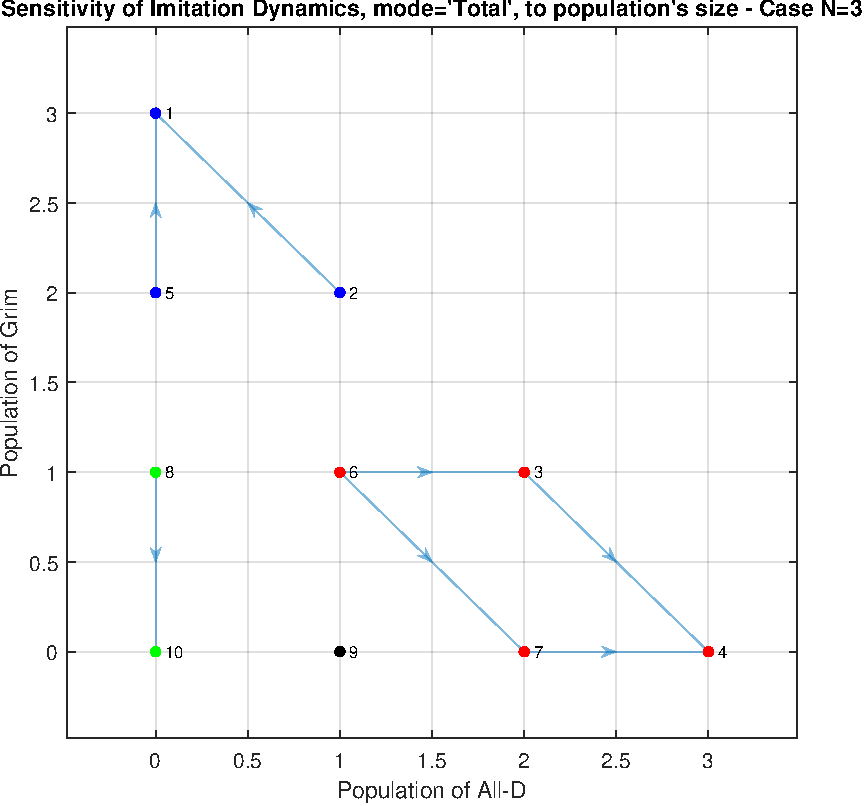
\includegraphics[height=0.9\textwidth]{Sensitivity of Imitation Dynamics, mode='Total', to population's size - Case N=3}
			\caption{Case $N=3$}
			\label{fig:example26}
		\end{subfigure}
		\begin{subfigure}[t]{.49\textwidth}
			\centering
			\includegraphics[height=0.9\textwidth]{Sensitivity of Imitation Dynamics, mode='Total', to population's size - Case N=5}
			\caption{Case $N=5$}
			\label{fig:example27}
		\end{subfigure}
		\begin{subfigure}[t]{.49\textwidth}
			\centering
			\includegraphics[height=0.9\textwidth]{Sensitivity of Imitation Dynamics, mode='Total', to population's size - Case N=10}
			\caption{Case $N=10$}
			\label{fig:example28}
		\end{subfigure}
		\begin{subfigure}[t]{.49\textwidth}
			\centering
			\includegraphics[height=0.9\textwidth]{Sensitivity of Imitation Dynamics, mode='Total', to population's size - Case N=3}
			\caption{Case $N=100$}
			\label{fig:example29}
		\end{subfigure}
		\caption{Sensitivity of Imitation Dynamics (mode=``Total'') to population size for $B = \begin{bmatrix} 3 & 1 \\ 4 & 2 \end{bmatrix}$}
		\label{fig:Sensitivity of Imitation Dynamics, mode='Total', to population's size}
	\end{figure}
	
	\begin{figure}[h]
		\centering
		\begin{subfigure}{.49\textwidth}
			\centering
			\includegraphics[height=0.9\textwidth]{Sensitivity of Imitation Dynamics, mode='Total', to payoff matrix - Case a=3.2}
			\caption{Case $a=3.2$}
			\label{fig:example30}
		\end{subfigure}
		\begin{subfigure}{.49\textwidth}
			\centering
			\includegraphics[height=0.9\textwidth]{Sensitivity of Imitation Dynamics, mode='Total', to payoff matrix - Case a=3.4}
			\caption{Case $a=3.4$}
			\label{fig:example31}
		\end{subfigure}
		\vspace{0.5em}
		\begin{subfigure}{.49\textwidth}
			\centering
			\includegraphics[height=0.9\textwidth]{Sensitivity of Imitation Dynamics, mode='Total', to payoff matrix - Case a=3.6}
			\caption{Case $a=3.6$}
			\label{fig:example32}
		\end{subfigure}
		\begin{subfigure}{.49\textwidth}
			\centering
			\includegraphics[height=0.9\textwidth]{Sensitivity of Imitation Dynamics, mode='Total', to payoff matrix - Case a=3.8}
			\caption{Case $a=3.8$}
			\label{fig:example33}
		\end{subfigure}
		\caption{Sensitivity of Imitation Dynamics (mode=``Total'') to payoff matrix parameter $a$ for $B = \begin{bmatrix} a & 1 \\ 4 & 2 \end{bmatrix}$ and $N=10$}
		\label{fig:Sensitivity of Imitation Dynamics, mode='Total', to payoff matrix}
	\end{figure}
 % Include the Imitation Dynamics chapter
\section{Discussion}
\subsection{Σύγκριση Fitness vs Imitation Dynamics}
	\begin{figure}[h]
	      \centering
	      \includegraphics[width=0.9\textwidth]{Fitness Dynamics vs Imitation Dynamics.pdf}
	      \caption{Fitness Dynamics vs Imitation Dynamics $\begin{bmatrix}All\_D&All\_C&TitForTat\end{bmatrix}$ $POP0=\begin{bmatrix}4&6&4\end{bmatrix}$}
	      \label{fig:Fitness Dynamics vs Imitation Dynamics}
	\end{figure}
Στο Σχήμα \ref{fig:Fitness Dynamics vs Imitation Dynamics} γίνεται μία σύγκριση μεταξύ των αποτελεσμάτων των TourSimFit, TourSimImi με mode=''Individual'' και TourSimImi με mode=''Total'' για στρατηγικές $\begin{bmatrix}All\_D&All\_C&TitForTat\end{bmatrix}$ με $POP0=\begin{bmatrix}4&6&4\end{bmatrix}$.
Παρατηρούμε ότι η περίπτωση Fitness μοιάζει με την περίπτωση ``Individual'' mode, ωστόσο και μεταξύ των δύο σημειώνεται η σημαντική διαφορά ότι στα Imitation Dynamics επιβιώνει μόνο μία στρατηγική. Η περίπτωση του ``Total'' mode έχει παρόμοια εξέλιξη με το ``Individual'' mode αλλά παρατηρούμε ότι επιβιώνει διαφορετική στρατηγική, συγκεκριμένα η ``All\_C'', επειδή έχει αρχικό πληθυσμό μεγαλύτερο από τις άλλες στρατηγικές και άρα εκμεταλλεύεται καλύτερα την συμπαθή στρατηγική ``TitForTat'' μέσω της λειτουργίας του ``Total'' mode για εύρεση της βέλτιστης στρατηγικής.

\subsection{Τελικά Συμπεράσματα}
Από την παραπάνω ανάλυση των δύο εξελικτικών δυναμικών προκύπτουν τα παρακάτω συμπεράσματα:

\subsubsection*{Για τα Fitness Dynamics}
α) Οι Mathieu et al φαίνεται ότι χρησιμοποιούσαν απλό floor κατά τον υπολογισμό των νέων πληθυσμών μετά από κάθε γενιά, καθώς η τακτική αυτή δημιούργησε για εμάς τα κοντινότερα αποτελέσματα.

β) Σε πολλές περιπτώσεις ασταθών, γενικά, συμπεριφορών, τα διαγράμματα διαφοροποιούνται σε παρατηρήσιμο βαθμό ανάλογα με το αν χρησιμοποιείται η συνάρτηση TourTheFit ή η συνάρτηση TourSimFit με και χωρίς compensation. Αυτό οφείλεται στο ότι πολλές από τις περιπτώσεις των διαγραμμάτων που προκύπτουν είναι ιδιαίτερα ευαίσθητες και έτσι, ακόμα και μικρή μεταβολή στη λογική της δυναμικής, μπορεί να αλλάξει τα αποτελέσματα σημαντικά.

γ) Το διάγραμμα που προκύπτει εξαρτάται από τις αρχικές τιμές πληθυσμού, τις στρατηγικές που χρησιμοποιούνται και τον πίνακα απολαβής. Ακόμα και για 2 από αυτούς τους παράγοντες ίδιους, η μεταβολή ενός από αυτούς μπορεί να οδηγήσει σε δραστικά διαφορετικά αποτελέσματα (ακόμα και διαφορετική ταξινόμηση, όπως στην 5η προσομοίωση).

δ) Η ανάθεση των εναπομείναντων μελών του πληθυσμού τυχαία σύμφωνα με τη λογική του compensation φαίνεται να είναι καλή επιλογή, ειδικά σε σχέση με την απλότητά της, διότι δε μεταβάλλει σημαντικά τα αποτελέσματα (στρατηγικές που θεωρητικά πεθαίνουν, πεθαίνουν πραγματικά, γενικά το πού τείνουν οι πληθυσμοί δεν αλλάζει). Ανάλογα με την περίπτωση που εξετάζεται, μοιάζει περισσότερο είτε με την περίπτωση της TourTheFit είτε με την περίπτωση TourSimFit δίχως compensation.

ε) Σε γενικές γραμμές, η διακριτή φύση των προσομοιώσεων TourSimFit με ή χωρίς compensation, δημιουργεί σε βάθος χρόνου είτε επαναλαμβανόμενες ταλαντώσεις είτε σύγκλιση σε κάποιες τελικές τιμές πληθυσμού. Το χάος δεν μπορεί πραγματικά να επιτευχθεί, ακόμα και στην 6η προσομοίωση οι πληθυσμοί τελικά τείνουν στις τιμές που προβλέπει και η TourTheFit. Ωστόσο, αυτό δε μας αποτρέπει από το να δημιουργήσουμε τα ενδιαφέροντα αποτελέσματα που βλέπουμε και στο paper.

\subsubsection*{Για τα Imitation Dynamics}
α) Η επιλογή της ακριβής δυναμικής που ακολουθάται κατά τον υπολογισμό των πληθυσμών της επόμενης γενιάς είναι βασική για τα αποτελέσματα που προκύπτουν. Για παράδειγμα, η επιλογή K παικτών από τον συνολικό πληθυσμό ή K παικτών εκ των μη βέλτιστων, δημιουργούν πολύ διαφορετικά αποτελέσματα και θεωρητικά και στις προσομοιώσεις.

β) Οι περιπτώσεις υπολογισμού της βέλτιστης στρατηγικής με τη μέθοδο In\-di\-vi\-du\-al και Total οδηγούν επίσης σε δραστικά διαφορετικά αποτελέσματα για τη φύση των καταστάσεων που προκύπτουν, όπως φαίνεται στις προσομοιώσεις 2 και 3. Σε γενικές γραμμές, η μέθοδος Total δημιουργεί συνεκτικούς υπογράφους που έχουν ως τελικές καταστάσεις τις καταστάσεις επικράτησης μίας εκ των στρατηγικών, ενώ η μέθοδος Individual δημιουργεί έναν μεγαλύτερο υπογράφο που οδηγεί σε πολλές πιθανές τελικές καταστάσεις και μερικές απομονωμένες τελικές καταστάσεις. Ο όρος συνεκτικότητα χρησιμοποιείται εδώ λανθασμένα, καθώς πρόκειται για κατευθυνόμενους γράφους στους οποίους κατά κανόνα δεν υπάρχουν διαδρομές και προς τις δύο κατευθύνσεις, αλλά χρησιμοποιείται για τη χαλαρή επεξήγηση του φαινομένου.

γ) Λόγω του β), παρατηρούμε ότι η τελική κατάσταση δεν είναι πάντα βέβαιη γνωρίζοντας την αρχική, εφόσον επιλέγεται η μέθοδος Individual. Αυτό οφείλεται στο ότι η τυχαία ανάθεση ανά γενιά μπορεί να οδηγήσει διαφορετικές κάθε φορά στρατηγικές σε πλεονεκτική θέση την επόμενη γενιά, και άρα να υπάρχει μεταβλητότητα στα αποτελέσματα. Αντιθέτως, η μέθοδος Total είναι πλήρως ντετερμινιστική ως προς την αρχική και τελική κατάσταση, ενώ παρουσιάζει τυχαιότητα μόνο στο μονοπάτι που θα ακολουθηθεί μεταξύ των 2.

δ) Σε κάθε περίπτωση, οι πληθυσμοί που προκύπτουν από τη συνάρτηση Tour\-Sim\-Imi ακολουθούν κάποια σειρά μεταβολών που παρουσιάζεται στο διάγραμμα μετάβασης καταστάσεων της αντίστοιχης Tour\-The\-Imi και Analyze\-Markov\-Chain.
 % Include the Discussion chapter

\clearpage
\nocite{*}
\bibliographystyle{plain}
\bibliography{Chapters/References}

\section{Appendices}
\subsection{Documentation}
{
\titleformat{\paragraph}
{\normalfont\normalsize\bfseries}{\theparagraph}{1em}{}
\titlespacing*{\paragraph}
{0pt}{1em}{1em}

\let\section\subsubsection
\let\subsection\paragraph

\section{Introduction}
The following is a file containing the documentation for the Evolutionary Games Toolbox contained in this GitHub repository. It is split into three segments: in the first segment, the documentation of each function contained in the Code folder are presented, whereas in the second segment, the simulation correspoding to each example file in the Examples folder is noted. Lastly, the third segment contains documentation on the strategies in the strategies subfolder of the Code folder. Note that the details regarding the operation of each function are not presented in this file (a lot of this is done in the Report.pdf file in the Report folder). Instead, this is a showcase of what each function expects as input, what it returns as output, which example corresponds to which simulation and how each strategy of the toolbox behaves. Across the functions written, there are smaller helper functions that are not included in this documentation, for the sake of simplicity.

\section{Functions of Code folder}
This is the documentation of the functions contained in the Code folder. The inputs/outputs of each functions are presented, without showcasing the operation of each one. See also the Report.pdf as well as the source code of each function (it is properly commented) if necessary.

\subsection{AnalyzeMarkovChain}
The AnalyzeMarkovChain function is responsible for creating the directed state graphs of the Imitation Dynamics. It requires inputs $P$ the transition matrix of the Markov Chain (usually calculated by the TourTheImi function), $POP0$ the initial $1 \times S$ (with $S$ the number of strategies used in the simulation) population vector, $Strategies$ an array containing the string names of the strategies used in the simulation (as named later on in the Strategies section) and $Title$ the string containing the title of the outgoing graph. The function does not have any outputs, as it only creates the graph and exports it for use in the Report).

\subsection{Axel}
The Axel function computes the score of a single generation Axelrod tournament between specific strategies. It expects inputs $B$ a $2 \times 2$ payoff matrix for each match, $Strategies$ an array containing the string names of the strategies used in the simulation (as named later on in the Strategies section), $Pop$ the initial $1 \times S$ (with $S$ the number of strategies used in the simulation) population vector and $T$ the number of rounds played in each match of the tournament. It returns an $N \times 1$ array (with $N$ being the total number of players in the simulation) containing the score of each player of the simulation at the end of the Axelrod tournament. Note that this function is not used for functions later on because of other faster implementations used.

\subsection{plotFitnessVSImitation}
The plotFitnessVSImitation function creates and exports a figure comparing the Fitness and Imitation Dynamics, using both ``Total'' and ``Individual'' mode for best strategy calculation in the Imitation Dynamics. It expects inputs $Strategies$ an array containing the string names of the strategies used in the simulation (as named later on in the Strategies section), $POP1$ the population matrix for each generation of the Fitness Dynamics (created by TourSimFit), $POP2$ the population matrix for each generation of the Imitation Dynamics - ``Individual'' mode (created by TourSimImi), $POP3$ the population matrix for each generation of the Imitation Dynamics - ``Total'' mode (created by TourSimImi with ``Total'' mode input) and $Title$ the title string of the created graph. The function does not have outputs and only creates and exports the graph. See example10 for an example usage of the function.

\subsection{plotPopulationOfStrategiesOverGenerations}
The plotPopulationOfStrategiesOverGenerations function constructs the diagram of populations of different strategies across generations after a completed simulation. It requires inputs $Strategies$ an array containing the string names of the strategies used in the simulation (as named later on in the Strategies section), $POP$ the population matrix for each generation of the given simulation, created by the corresponding function and $Title$ the title string of the created diagram. The function does not have outputs and only creates and exports the diagram graphing the population of each strategy with respect to the generation number.

\subsection{plotPopulationsOfStrategiesOverGenerations}
The plotPopulationsOfStrategiesOverGenerations function creates the plots for the population of different strategies across generations for results generated by TourTheFit, TourSimFit with compensation and without compensation. It expects inputs $Strategies$ an array containing the string names of the strategies used in the simulation (as named later on in the Strategies section), $POP1$ the theoretical population matrix for each generation of the Fitness Dynamics (created by TourTheFit), $POP2$ the population matrix for each generation of the Fitness Dynamics without compensation (created by TourSimFit), $POP3$ the population matrix for each generation of the Fitness Dynamics with compensation (created by TourSimFit with $compensation$ = true input) and $Title$ the title string of the created figure. The function does not have outputs and only creates and exports the figure. See the first few examples for example usages of the function.

\subsection{plotPopulationsTourSimImi}
The plotPopulationsTourSimImi function creates the plot for the population of different strategies across generations after a completed TourSimImi simulation. It expects inputs $Strategies$ an array containing the string names of the strategies used in the simulation (as named later on in the Strategies section), $POP$ the population matrix for each generation of the given simulation, created by the TourSimImi function and $Title$ the title string of the created plot. The function does not have outputs and only creates and exports the diagram graphing the population of each strategy with respect to the generation number. See example07 for an example usage of the function.

\subsection{TourSimFit}
The TourSimFit function simulates the evolutionary tournament using Fitness Dynamics. The function expects inputs $B$ a $2 \times 2$ payoff matrix for each match, $Strategies$ an array containing the string names of the strategies used in the simulation (as named later on in the Strategies section), $POP0$ the initial $1 \times S$ (with $S$ the number of strategies used in the simulation) population vector, $T$ the number of rounds played in each match of the tournament, $J$ the number of generations of the simulation and $compensation$ an optional argument (with default value being false) that toggles the usage of random compensation to keep the total population of each generation constant (this is better explained in the Report). It returns a $(J+1) \times S$ array $POP$ containing the population of each generation for each strategy, a $J \times S$ array $BST$ containing information about the best strategy of each generation (for the cell $(i,j)$ of the array, if it has value 1 then strategy $j$ was the best for generation $i$, else it has value 0) and $FIT$ a $J \times S$ array that contains the fitness scores of each strategy for each generation.

\subsection{TourSimImi}
The TourSimImi function simulates the evolutionary tournament using Imitation Dynamics. The function expects inputs $B$ a $2 \times 2$ payoff matrix for each match, $Strategies$ an array containing the string names of the strategies used in the simulation (as named later on in the Strategies section), $POP0$ the initial $1 \times S$ (with $S$ the number of strategies used in the simulation) population vector, $T$ the number of rounds played in each match of the tournament, $J$ the number of generations of the simulation and $mode$ an optional argument (with default value being ``Individual'') that toggles the mode for best strategy selection, with the other option being ``Total'' (this is better explained in the Report). It returns a $(J+1) \times S$ array $POP$ containing the population of each generation for each strategy and a $J \times S$ array $BST$ containing information about the best strategy of each generation (for the cell $(i,j)$ of the array, if it has value 1 then strategy $j$ was the best for generation $i$, else it has value 0).

\subsection{TourTheFit}
The TourTheFit function conducts the theoretical analysis of an evolutionary tournament using Fitness Dynamics. The function expects inputs $B$ a $2 \times 2$ payoff matrix for each match, $Strategies$ an array containing the string names of the strategies used in the simulation (as named later on in the Strategies section), $POP0$ the initial $1 \times S$ (with $S$ the number of strategies used in the simulation) population vector, $T$ the number of rounds played in each match of the tournament and $J$ the number of generations of the simulation. It returns a $(J+1) \times S$ array $POP$ containing the population of each generation for each strategy, a $J \times S$ array $BST$ containing information about the best strategy of each generation (for the cell $(i,j)$ of the array, if it has value 1 then strategy $j$ was the best for generation $i$, else it has value 0) and $FIT$ a $J \times S$ array that contains the fitness scores of each strategy for each generation.

\subsection{TourTheImi}
The function TourTheImi computes the state transition matrix of a given evolutionary tournament using Imitation Dynamics using Markov Chain theory. The function expects inputs $B$ a $2 \times 2$ payoff matrix for each match, $Strategies$ an array containing the string names of the strategies used in the simulation (as named later on in the Strategies section), $POP0$ the initial $1 \times S$ (with $S$ the number of strategies used in the simulation) population vector, $T$ the number of rounds played in each match of the tournament, $J$ the number of generations of the simulation and $mode$ an optional argument (with default value being ``Individual'') that toggles the mode for best strategy selection, with the other option being ``Total'' (this is better explained in the Report). It returns an array $P$ which is the state transition matrix of the process. More specifically, the cell $(i,j)$ of the array contains the probability that the system reaches state $j$ at the next step, given that the system starts at state $i$ (with system being the population distribution and each state being each possible population distribution). Use AnalyzeMarkovChain to visualize and understand the results.

\section{Examples of Examples folder}
This is the documentation of the Examples contained in the Examples folder of the repository. More specifically, the situation each example simulates is presented and any possible links to the paper by Mathieu et al are mentioned.

\subsection{example01}
The first example shows the results of TourTheFit, TourSimFit with compensation and TourSimFit without compensation in the case presented by Mathieu et al in Figure 1, with Title ``Defectors may be strong''. The functions are called with payoff matrix $B = \begin{bmatrix} 3 & 0 \\ 5 & 1 \end{bmatrix}$, $Strategies = ["per\_ddc", "Alternator", "soft\_majo"]$, initial population $POP0 = [100; 100; 100]$, number of rounds per match $T = 1000$ and number of generations $J = 90$.

\subsection{example02}
This shows the results of TourTheFit, TourSimFit with compensation and TourSimFit without compensation in the case presented by Mathieu et al in Figure 2, with Title ``Monotonous convergence''. The functions are called with payoff matrix $B = \begin{bmatrix} 3 & 0 \\ 5 & 1 \end{bmatrix}$, $Strategies = ["Grim", "TitForTat", "Alternator"]$, initial population $POP0 = [100; 100; 100]$, number of rounds per match $T = 1000$ and number of generations $J = 10$.

\subsection{example03}
This shows the results of TourTheFit, TourSimFit with compensation and TourSimFit without compensation in the case presented by Mathieu et al in Figure 3, with Title ``Attenuated oscillatory movements''. The functions are called with payoff matrix $B = \begin{bmatrix} 3 & 0 \\ 5 & 1 \end{bmatrix}$, $Strategies = ["per\_ccd", "per\_ddc", "soft\_majo"]$, initial population $POP0 = [450; 1000; 100]$, number of rounds per match $T = 1000$ and number of generations $J = 420$.

\subsection{example04}
This shows the results of TourTheFit, TourSimFit with compensation and TourSimFit without compensation in the case presented by Mathieu et al in Figure 4, with Title ``Periodic movements''. The functions are called with payoff matrix $B = \begin{bmatrix} 3 & 0 \\ 5 & 1 \end{bmatrix}$, $Strategies = ["per\_ccd", "per\_ddc", "soft\_majo"]$, initial population $POP0 = [300; 200; 100]$, number of rounds per match $T = 1000$ and number of generations $J = 1000$.

\subsection{example05}
This shows the results of TourTheFit, TourSimFit with compensation and TourSimFit without compensation in the case presented by Mathieu et al in Figure 5, with Title ``Increasing oscillations''. The functions are called with payoff matrix $B = \begin{bmatrix} 3 & 0 \\ 5 & 1 \end{bmatrix}$, $Strategies = ["Alternator", "per\_ddc", "soft\_majo"]$, initial population $POP0 = [400; 300; 200]$, number of rounds per match $T = 1000$ and number of generations $J = 450$.

\subsection{example06}
This shows the results of TourTheFit, TourSimFit with compensation and TourSimFit without compensation in the case presented by Mathieu et al in Figure 6, with Title ``Disordered oscillations''. The functions are called with payoff matrix $B = \begin{bmatrix} 3 & 0 \\ 5 & 1 \end{bmatrix}$, $Strategies = ["soft\_majo", "per\_ccccd", "Prober"]$, initial population $POP0 = [100; 500; 800]$, number of rounds per match $T = 1000$ and number of generations $J = 280$.

\subsection{example07}
This shows the results of TourTheFit, TourSimFit with compensation and TourSimFit without compensation in the case presented by Mathieu et al in the left plot of Figure 7, with Title ``Sensitivity of dynamics to population's size''. The functions are called with payoff matrix $B = \begin{bmatrix} 3 & 0 \\ 5 & 1 \end{bmatrix}$, $Strategies = ["per\_ccd", "soft\_majo", "per\_ddc"]$, initial population $POP0 = [300; 100; 244]$, number of rounds per match $T = 1000$ and number of generations $J = 1000$.

\subsection{example08}
This shows the results of TourTheFit, TourSimFit with compensation and TourSimFit without compensation in the case presented by Mathieu et al in the right plot of Figure 7, with Title ``Sensitivity of dynamics to population's size''. The functions are called with payoff matrix $B = \begin{bmatrix} 3 & 0 \\ 5 & 1 \end{bmatrix}$, $Strategies = ["per\_ccd", "soft\_majo", "per\_ddc"]$, initial population $POP0 = [300; 100; 245]$, number of rounds per match $T = 1000$ and number of generations $J = 1000$.

\subsection{example09}
This shows the results of TourTheFit, TourSimFit with compensation and TourSimFit without compensation in the case presented by Mathieu et al in the left plot of Figure 8, with Title ``Sensitivity of winner to population's size''. The functions are called with payoff matrix $B = \begin{bmatrix} 3 & 0 \\ 5 & 1 \end{bmatrix}$, $Strategies = ["per\_ddc", \- "soft\_majo", \-"Alternator"]$, initial population $POP0 = [100; 159; 100]$, number of rounds per match $T = 1000$ and number of generations $J = 120$.

\subsection{example10}
This shows the results of TourTheFit, TourSimFit with compensation and TourSimFit without compensation in the case presented by Mathieu et al in the right plot of Figure 8, with Title ``Sensitivity of winner to population's size''. The functions are called with payoff matrix $B = \begin{bmatrix} 3 & 0 \\ 5 & 1 \end{bmatrix}$, $Strategies = ["per\_ddc", "soft\_majo", "Alternator"]$, initial population $POP0 = [100; 160; 100]$, number of rounds per match $T = 1000$ and number of generations $J = 120$.

\subsection{example11}
This shows the results of TourTheFit, TourSimFit with compensation and TourSimFit without compensation in the case presented by Mathieu et al in the left plot of Figure 9, with Title ``Sensitivity to game length''. The functions are called with payoff matrix $B = \begin{bmatrix} 3 & 0 \\ 5 & 1 \end{bmatrix}$, $Strategies = ["per\_ccd", "soft\_majo", "per\_ddc"]$, initial population $POP0 = [300; 100; 244]$, number of rounds per match $T = 7$ and number of generations $J = 1000$.

\subsection{example12}
This shows the results of TourTheFit, TourSimFit with compensation and TourSimFit without compensation in the case presented by Mathieu et al in the right plot of Figure 9, with Title ``Sensitivity to game length''. The functions are called with payoff matrix $B = \begin{bmatrix} 3 & 0 \\ 5 & 1 \end{bmatrix}$, $Strategies = ["per\_ccd", "soft\_majo", "per\_ddc"]$, initial population $POP0 = [300; 100; 244]$, number of rounds per match $T = 6$ and number of generations $J = 1000$.

\subsection{example13}
This shows the results of TourTheFit, TourSimFit with compensation and TourSimFit without compensation in the case presented by Mathieu et al in the left plot of Figure 10, with Title ``Sensitivity to CIPD payoff''. The functions are called with payoff matrix $B = \begin{bmatrix} 3 & 0 \\ 4.6 & 1 \end{bmatrix}$, $Strategies = ["per\_ccd", "soft\_majo", "per\_ddc"]$, initial population $POP0 = [300; 100; 244]$, number of rounds per match $T = 1000$ and number of generations $J = 475$.

\subsection{example14}
This shows the results of TourTheFit, TourSimFit with compensation and TourSimFit without compensation in the case presented by Mathieu et al in the right plot of Figure 10, with Title ``Sensitivity to CIPD payoff''. The functions are called with payoff matrix $B = \begin{bmatrix} 3 & 0 \\ 4.7 & 1 \end{bmatrix}$, $Strategies = ["per\_ccd", "soft\_majo", "per\_ddc"]$, initial population $POP0 = [300; 100; 244]$, number of rounds per match $T = 1000$ and number of generations $J = 1000$.

\subsection{example15}
This shows the results of TourTheFit, TourSimFit with compensation and TourSimFit without compensation in the case presented by Mathieu et al in the plots of Figure 11, with Title ``Sensitivity to repartition computation method''. The functions are called with payoff matrix $B = \begin{bmatrix} 3 & 0 \\ 5 & 1 \end{bmatrix}$, $Strategies = ["per\_ccd", \- "soft\_majo", "per\_ddc"]$, initial population $POP0 = [300; 100; 200]$, number of rounds per match $T = 1000$ and number of generations $J = 1000$. Note that the plot on the left corresponds to the plot created by TourSimFit and the plot on the right corresponds to the one created by TourTheFit.

\subsection{example16}
This shows the results of TourTheFit, TourSimFit with compensation and TourSimFit without compensation in the case presented by Mathieu et al in the left plot of Figure 12, with Title ``Sensitivity to repartition computation method''. The functions are called with payoff matrix $B = \begin{bmatrix} 3 & 0 \\ 4.6 & 1 \end{bmatrix}$, $Strategies = ["per\_ccd", "soft\_majo", "per\_ddc"]$, initial population $POP0 = [450; 100; 1000]$, number of rounds per match $T = 1000$ and number of generations $J = 1000$.

\subsection{example17}
This shows the results of TourTheFit, TourSimFit with compensation and TourSimFit without compensation in the case presented by Mathieu et al in the right plot of Figure 12, with Title ``Sensitivity to repartition computation method''. The functions are called with payoff matrix $B = \begin{bmatrix} 3 & 0 \\ 4.6 & 1 \end{bmatrix}$, $Strategies = ["per\_ccd", "soft\_majo", "per\_ddc"]$, initial population $POP0 = [45; 10; 100]$, number of rounds per match $T = 1000$ and number of generations $J = 1000$.

\subsection{example18}
This showcases the sensitivity of Imitation Dynamics, mode = ``Individual'' to the population's size, in the case $N=3$. The function TourTheImi is called with payoff matrix $B = \begin{bmatrix} 3 & 1 \\ 4 & 2 \end{bmatrix}$, $Strategies = ["All\_C", "All\_D", "Grim"]$, initial population $POP0 = [0; 0; 3]$, number of imitators per round $K=1$, number of rounds per match $T = 100$ and number of generations $J = 15$. The function PlotStateTransitionGraph is then called with arguments state transition matrix $P$ as calculated by TourTheImi, initial population $POP0 = [0; 0; 3]$, $Strategies = ["All\_C", "All\_D", "Grim"]$ and a proper title.

\subsection{example19}
This showcases the sensitivity of Imitation Dynamics, mode = ``Individual'' to the population's size, in the case $N=5$. The function TourTheImi is called with payoff matrix $B = \begin{bmatrix} 3 & 1 \\ 4 & 2 \end{bmatrix}$, $Strategies = ["All\_C", "All\_D", "Grim"]$, initial population $POP0 = [0; 0; 5]$, number of imitators per round $K=1$, number of rounds per match $T = 100$ and number of generations $J = 15$. The function PlotStateTransitionGraph is then called with arguments state transition matrix $P$ as calculated by TourTheImi, initial population $POP0 = [0; 0; 5]$, $Strategies = ["All\_C", "All\_D", "Grim"]$ and a proper title.

\subsection{example20}
This showcases the sensitivity of Imitation Dynamics, mode = ``Individual'' to the population's size, in the case $N=10$. The function TourTheImi is called with payoff matrix $B = \begin{bmatrix} 3 & 1 \\ 4 & 2 \end{bmatrix}$, $Strategies = ["All\_C", "All\_D", "Grim"]$, initial population $POP0 = [0; 0; 10]$, number of imitators per round $K=1$, number of rounds per match $T = 100$ and number of generations $J = 15$. The function PlotStateTransitionGraph is then called with arguments state transition matrix $P$ as calculated by TourTheImi, initial population $POP0 = [0; 0; 10]$, $Strategies = ["All\_C", "All\_D", "Grim"]$ and a proper title.

\subsection{example21}
This showcases the sensitivity of Imitation Dynamics, mode = ``Individual'' to the population's size, in the case $N=100$. The function TourTheImi is called with payoff matrix $B = \begin{bmatrix} 3 & 1 \\ 4 & 2 \end{bmatrix}$, $Strategies = ["All\_C", "All\_D", "Grim"]$, initial population $POP0 = [0; 0; 100]$, number of imitators per round $K=1$, number of rounds per match $T = 100$ and number of generations $J = 15$. The function PlotStateTransitionGraph is then called with arguments state transition matrix $P$ as calculated by TourTheImi, initial population $POP0 = [0; 0; 100]$, $Strategies = ["All\_C", "All\_D", "Grim"]$ and a proper title.

\subsection{example22}
This showcases the sensitivity of Imitation Dynamics, mode = ``Individual'' to the payoff matrix, in the case $a = 3.2$. The function TourTheImi is called with payoff matrix $B = \begin{bmatrix} 3.2 & 1 \\ 4 & 2 \end{bmatrix}$, $Strategies = ["All\_C", "All\_D", "Grim"]$, initial population $POP0 = [0; 0; 10]$, number of imitators per round $K=1$, number of rounds per match $T = 100$ and number of generations $J = 15$. The function PlotStateTransitionGraph is then called with arguments state transition matrix $P$ as calculated by TourTheImi, initial population $POP0 = [0; 0; 10]$, $Strategies = ["All\_C", "All\_D", "Grim"]$ and a proper title.

\subsection{example23}
This showcases the sensitivity of Imitation Dynamics, mode = ``Individual'' to the payoff matrix, in the case $a = 3.4$. The function TourTheImi is called with payoff matrix $B = \begin{bmatrix} 3.4 & 1 \\ 4 & 2 \end{bmatrix}$, $Strategies = ["All\_C", "All\_D", "Grim"]$, initial population $POP0 = [0; 0; 10]$, number of imitators per round $K=1$, number of rounds per match $T = 100$ and number of generations $J = 15$. The function PlotStateTransitionGraph is then called with arguments state transition matrix $P$ as calculated by TourTheImi, initial population $POP0 = [0; 0; 10]$, $Strategies = ["All\_C", "All\_D", "Grim"]$ and a proper title.

\subsection{example24}
This showcases the sensitivity of Imitation Dynamics, mode = ``Individual'' to the payoff matrix, in the case $a = 3.6$. The function TourTheImi is called with payoff matrix $B = \begin{bmatrix} 3.6 & 1 \\ 4 & 2 \end{bmatrix}$, $Strategies = ["All\_C", "All\_D", "Grim"]$, initial population $POP0 = [0; 0; 10]$, number of imitators per round $K=1$, number of rounds per match $T = 100$ and number of generations $J = 15$. The function PlotStateTransitionGraph is then called with arguments state transition matrix $P$ as calculated by TourTheImi, initial population $POP0 = [0; 0; 10]$, $Strategies = ["All\_C", "All\_D", "Grim"]$ and a proper title.

\subsection{example25}
This showcases the sensitivity of Imitation Dynamics, mode = ``Individual'' to the payoff matrix, in the case $a = 3.8$. The function TourTheImi is called with payoff matrix $B = \begin{bmatrix} 3.8 & 1 \\ 4 & 2 \end{bmatrix}$, $Strategies = ["All\_C", "All\_D", "Grim"]$, initial population $POP0 = [0; 0; 10]$, number of imitators per round $K=1$, number of rounds per match $T = 100$ and number of generations $J = 15$. The function PlotStateTransitionGraph is then called with arguments state transition matrix $P$ as calculated by TourTheImi, initial population $POP0 = [0; 0; 10]$, $Strategies = ["All\_C", "All\_D", "Grim"]$ and a proper title.

\subsection{example26}
This showcases the sensitivity of Imitation Dynamics, mode = ``Total'' to the population's size, in the case $N=3$. The function TourTheImi is called with payoff matrix $B = \begin{bmatrix} 3 & 1 \\ 4 & 2 \end{bmatrix}$, $Strategies = ["All\_C", "All\_D", "Grim"]$, initial population $POP0 = [0; 0; 3]$, number of imitators per round $K=1$, number of rounds per match $T = 100$ and number of generations $J = 15$. The function PlotStateTransitionGraph is then called with arguments state transition matrix $P$ as calculated by TourTheImi, initial population $POP0 = [0; 0; 3]$, $Strategies = ["All\_C", "All\_D", "Grim"]$ and a proper title.

\subsection{example27}
This showcases the sensitivity of Imitation Dynamics, mode = ``Total'' to the population's size, in the case $N=5$. The function TourTheImi is called with payoff matrix $B = \begin{bmatrix} 3 & 1 \\ 4 & 2 \end{bmatrix}$, $Strategies = ["All\_C", "All\_D", "Grim"]$, initial population $POP0 = [0; 0; 5]$, number of imitators per round $K=1$, number of rounds per match $T = 100$ and number of generations $J = 15$. The function PlotStateTransitionGraph is then called with arguments state transition matrix $P$ as calculated by TourTheImi, initial population $POP0 = [0; 0; 5]$, $Strategies = ["All\_C", "All\_D", "Grim"]$ and a proper title.

\subsection{example28}
This showcases the sensitivity of Imitation Dynamics, mode = ``Total'' to the population's size, in the case $N=10$. The function TourTheImi is called with payoff matrix $B = \begin{bmatrix} 3 & 1 \\ 4 & 2 \end{bmatrix}$, $Strategies = ["All\_C", "All\_D", "Grim"]$, initial population $POP0 = [0; 0; 10]$, number of imitators per round $K=1$, number of rounds per match $T = 100$ and number of generations $J = 15$. The function PlotStateTransitionGraph is then called with arguments state transition matrix $P$ as calculated by TourTheImi, initial population $POP0 = [0; 0; 10]$, $Strategies = ["All\_C", "All\_D", "Grim"]$ and a proper title.

\subsection{example29}
This showcases the sensitivity of Imitation Dynamics, mode = ``Total'' to the population's size, in the case $N=100$. The function TourTheImi is called with payoff matrix $B = \begin{bmatrix} 3 & 1 \\ 4 & 2 \end{bmatrix}$, $Strategies = ["All\_C", "All\_D", "Grim"]$, initial population $POP0 = [0; 0; 100]$, number of imitators per round $K=1$, number of rounds per match $T = 100$ and number of generations $J = 15$. The function PlotStateTransitionGraph is then called with arguments state transition matrix $P$ as calculated by TourTheImi, initial population $POP0 = [0; 0; 100]$, $Strategies = ["All\_C", "All\_D", "Grim"]$ and a proper title.

\subsection{example30}
This showcases the sensitivity of Imitation Dynamics, mode = ``Total'' to the payoff matrix, in the case $a = 3.2$. The function TourTheImi is called with payoff matrix $B = \begin{bmatrix} 3.2 & 1 \\ 4 & 2 \end{bmatrix}$, $Strategies = ["All\_C", "All\_D", "Grim"]$, initial population $POP0 = [0; 0; 10]$, number of imitators per round $K=1$, number of rounds per match $T = 100$ and number of generations $J = 15$. The function PlotStateTransitionGraph is then called with arguments state transition matrix $P$ as calculated by TourTheImi, initial population $POP0 = [0; 0; 10]$, $Strategies = ["All\_C", "All\_D", "Grim"]$ and a proper title.

\subsection{example31}
This showcases the sensitivity of Imitation Dynamics, mode = ``Total'' to the payoff matrix, in the case $a = 3.4$. The function TourTheImi is called with payoff matrix $B = \begin{bmatrix} 3.4 & 1 \\ 4 & 2 \end{bmatrix}$, $Strategies = ["All\_C", "All\_D", "Grim"]$, initial population $POP0 = [0; 0; 10]$, number of imitators per round $K=1$, number of rounds per match $T = 100$ and number of generations $J = 15$. The function PlotStateTransitionGraph is then called with arguments state transition matrix $P$ as calculated by TourTheImi, initial population $POP0 = [0; 0; 10]$, $Strategies = ["All\_C", "All\_D", "Grim"]$ and a proper title.

\subsection{example32}
This showcases the sensitivity of Imitation Dynamics, mode = ``Total'' to the payoff matrix, in the case $a = 3.6$. The function TourTheImi is called with payoff matrix $B = \begin{bmatrix} 3.6 & 1 \\ 4 & 2 \end{bmatrix}$, $Strategies = ["All\_C", "All\_D", "Grim"]$, initial population $POP0 = [0; 0; 10]$, number of imitators per round $K=1$, number of rounds per match $T = 100$ and number of generations $J = 15$. The function PlotStateTransitionGraph is then called with arguments state transition matrix $P$ as calculated by TourTheImi, initial population $POP0 = [0; 0; 10]$, $Strategies = ["All\_C", "All\_D", "Grim"]$ and a proper title.

\subsection{example33}
This showcases the sensitivity of Imitation Dynamics, mode = ``Total'' to the payoff matrix, in the case $a = 3.8$. The function TourTheImi is called with payoff matrix $B = \begin{bmatrix} 3.8 & 1 \\ 4 & 2 \end{bmatrix}$, $Strategies = ["All\_C", "All\_D", "Grim"]$, initial population $POP0 = [0; 0; 10]$, number of imitators per round $K=1$, number of rounds per match $T = 100$ and number of generations $J = 15$. The function PlotStateTransitionGraph is then called with arguments state transition matrix $P$ as calculated by TourTheImi, initial population $POP0 = [0; 0; 10]$, $Strategies = ["All\_C", "All\_D", "Grim"]$ and a proper title.

\section{Strategies of strategies subfolder in the Code folder}
Lastly, this is the documentation for all strategies included in the strategies subfolder of the Code folder. For more details, the exact source code is available for each of the following strategies. Note that you can always enhance this collection with strategies of your own. For your created strategies to work with the toolbox, follow the format used in the strategies given: let the function have form function Move = YourStrategy(History), where History is the $T \times 2$ matrix of moves by both players for each turn, regard the player of your strategy as player 1 (the first column of the History matrix, it is flipped in case the player is actually player 2) and make Move = 2 in case of defection and Move = 1 in case of cooperation. Also, suppose that each strategy can only access past moves (player 2 cannot access player 1's current round move) and that each strategy does not know the amount of rounds played in each match. Lastly, because of the current form of simulation and theoretical analysis functions (that prioritize low running times), strategies including random elements are not included (in case you wish to include some, most functions will probably fail). For the strategies below, C stands for Cooperation and D stands for Defection.

\subsection{All\_C}
Strategy that always cooperates.

\subsection{All\_D}
Strategy that always defects.

\subsection{Alternator}
Strategy that alternates between cooperating and defecting, starting with cooperation in the first round.

\subsection{Cycler}
Strategy that permanently cycles the moves C, C, C, D.

\subsection{Detective}
Strategy that starts with the moves C, D, C, C. If the opponent defects at least once in these first four rounds, play as TitForTat forever. Else, always defect.

\subsection{Grim}
Strategy that always cooperates unless the opponent defects: after the first opponent defection, always defect.

\subsection{per\_ccccd}
Strategy that permanently cycles the moves C, C, C, C, D.

\subsection{per\_ccd}
Strategy that permanently cycles the moves C, C, D.

\subsection{per\_ddc}
Strategy that permanently cycles the moves D, D, C.

\subsection{Prober}
Strategy that starts with the moves D, C, C. If the opponent cooperates at moves 2 and 3, plays defect for the rest of the game. Otherwise plays as TitForTat.

\subsection{SneakyTitForTat}
Strategy that starts by cooperating in the first round and playing as TitForTat in the second round. If the opponent has not defected in these first two rounds, defect once and check the opponent's response. If the opponents retaliates, play a cooperation to repent and then play as TitForTat. If the opponent does not retaliate, keep playing defect and checking the opponent's response as before.

\subsection{soft\_majo}
Strategy that plays the same move as the majority of the opponent's moves up until the previous round. In case of equality, cooperate.

\subsection{SpitefulTitForTat}
Strategy that starts by cooperating and then plays like TitForTat, until the opponent defects twice in a row, in which case the player always defects.

\subsection{TitForTat}
Strategy that cooperates in the first move and for the rest of the game plays the opponent's previous move.

\subsection{TitForTwoTats}
Strategy that plays defect only if the opponent has defected twice in a row. Otherwise, always cooperates.

\subsection{TwoTitsForTat}
Strategy that starts by cooperating and replies to each opponent defection by two defections of its own. More specifically, if there has been a defection by the opponent in the two previous rounds, the player chooses defect. Otherwise, plays cooperate.

} % Include the Appendices chapter

\clearpage
\listoffigures
\end{document}